\documentclass[a4paper,12pt,oneside,titlepage]{book}
\usepackage{tikz}
\usepackage[T1]{fontenc}
\usepackage[utf8]{inputenc}
\usepackage[export]{adjustbox}
\usepackage{fixltx2e}
\usepackage{siunitx}
\usepackage[shortlabels]{enumitem}
\usepackage{csquotes}
\usepackage{graphicx}
\usepackage{appendix} 
\usepackage{longtable}
%\usepackage[ddmmyyyy]{datetime}
\usepackage{float}
\usepackage{wrapfig}
\usepackage{rotating}
\usepackage[normalem]{ulem}
\usepackage{amsmath}
\usepackage{enumitem}
\usepackage{textcomp}
\usepackage{marvosym}
\usepackage{wasysym}
\usepackage{amssymb}
\usepackage{multirow}
\usepackage{tabu}
\usepackage{marvosym}

\usepackage{minted}
\newcommand{\inline}[1]{\mintinline{Python}{#1}}
\graphicspath{ {./img/} }
\tolerance=1000
\usepackage[spanish,es-tabla,es-nodecimaldot]{babel}
\usepackage{a4wide}
\usepackage{gensymb}
\usepackage{wasysym}
\usepackage{subcaption}
\usepackage{braket}
\usepackage{amsthm}
\usepackage{mathtools}
\usepackage[backend=biber,sorting=none]{biblatex}
\usepackage[font=small,labelfont=bf]{caption}
% \usepackage[backend=biber]{biblatex}
% \usepackage{minted}
% \renewcommand{\appendixname}{Anexos}
% \renewcommand{\appendixtocname}{Anexos}
% \renewcommand{\appendixpagename}{Anexos}
\renewcommand{\chaptermark}[1]{\markboth{\thechapter.\ \chaptername.\ #1}{}}
\renewcommand{\sectionmark}[1]{\markright{\thesection\ #1}}
\addto\captionsspanish{%
\renewcommand\appendixname{Anexo}
\renewcommand\appendixpagename{Anexos}
}

\addbibresource{texto.bib}
\DeclareFieldFormat[article]{citetitle}{#1}
\DeclareFieldFormat[article]{title}{#1}
\DeclareFieldFormat{title}{#1}

% \newcommand{\inline}[1]{\mintinline{Python}{#1}}

\usepackage{setspace}
\usepackage[all]{nowidow}
\usepackage{hyperref}
\newcommand{\rcor}{\right\rbrace}
\newcommand{\lcor}{\left\lbrace }
\newcommand{\comen}{\textbf{Comentarios:}}
\author{Alejandro Ponce Miguela}
\date{}
\title{\textbf{Borrador TFM}}
\hypersetup{
  pdfkeywords={},
  pdfsubject={},
  pdfcreator={Alejandro Ponce Miguela}}
  \newtheorem{teor}{Teorema}
  \newtheorem{defi}{Definición}
  \newtheorem{lema}{Lema}
  \newtheorem{ejem}{Ejemplo}[subsection]
  \usepackage{tcolorbox}
  \usepackage{etoolbox}
  \newcommand{\red}[1]{\textcolor{red}{#1}}
  \newcommand{\blue}[1]{\textcolor{blue}{#1}}
  \BeforeBeginEnvironment{minted}{\begin{tcolorbox}}%
    \AfterEndEnvironment{minted}{\end{tcolorbox}}%
    
    \renewcommand\qedsymbol{$\blacksquare$}
    \setstretch{1.25}
    \setlength{\parskip}{1em}
    \interfootnotelinepenalty=10000
  \DefineBibliographyStrings{spanish}{andothers={\textit{et al.}}}
\begin{document}
\begin{titlepage}
  \begin{center}
      \vspace*{0.1cm}
      \includegraphics[scale=0.4]{img/logous.png}
       
       
       
      \Large\textbf{Universidad de Granada} \\
       
      
       
      Master en ciencia de datos e ingeniería de computadores \\
       
       
       
      Trabajo de Fin de Master \\
      \vspace{0.3cm}
      \rule{16cm}{0.3mm}
      
      \vspace{0.1cm}
      \scalebox{0.9}{
      \Large\textbf{Separación de cascadas electromagnéticas en el }}\\
      \scalebox{0.9}{
      
      \Large\textbf{experimento SBND mediante técnicas de Machine Learning}}

      \rule{16cm}{0.3mm}
      \large
      Autor: \\
      \textbf{Alejandro Ponce Miguela} \\
      \vspace{0.3cm}
      Tutores: \\
      \textbf{Alberto Guillén Perales} \\
      \textbf{Bruno Zamorano García} \\
      \vspace{0.3cm}
      Departamento de Arquitectura y Tecnología de Computadores \\
      \vspace{0.3cm}
      Escuela Técnica Superior de Ingenierías Informática y de Telecomunicaciones\\
      \today
  \end{center}
\end{titlepage}
\frontmatter
\newpage
\noindent
Don ALEJANDRO PONCE MIGUELA con D.N.I. 30235577, estudiante de master en la Universidad de Granada y autor del trabajo titulado Separación de cascadas electromagnéticas en el experimento SBND mediante técnicas de Machine Learning:
\\
\\
DECLARO
\\
\\
Que el trabajo fin de grado que he presentado para su evaluación es original y de elaboración personal, lo
que implica la no reproducción de fragmentos de obras no amparados por el límite de cita, regulado en el
artículo 32 de la Ley de Propiedad Intelectual, y no copio ni utilizo ideas, formulaciones, parafraseo,
etcétera, tomadas de cualquier obra, sin expresar de manera clara su origen tanto en el cuerpo del trabajo
como en su bibliografía.
\\
\\
De no cumplir con este requisito propio de cualquier trabajo académico, soy plenamente consciente que
ello conllevará automáticamente la calificación de NO APTO y, en su caso, podré ser objeto de sanción
académica, previa apertura de expediente disciplinario o de otro orden legal.
\\
\\
Sevilla, a 4 de julio de 2022.
\begin{figure}[h!]
  \includegraphics[scale=0.18]{Captura.PNG}
\end{figure}
\\
Don ALEJANDRO PONCE MIGUELA
\newpage

\section*{Resumen}
% En general esta creo que más o menos todo faltan algunos detalles:
% \begin{itemize}
  %   \item Quitar hits temporalmente.
%   \item Conclusiones y Abstract.
%   \item presupuesto
% \end{itemize}

% Como cosas adicionales que quiero hacer las últimas dos semanas (la semana que viene no puedo hacer nada). Sería:
% \begin{itemize}
%   \item resolver algunas cuestiones que están indicadas en el texto y me gustaría hablar con vosotros: por qué el eje $y$ es el mejor para la proyección, y el tema de las citas que me tiene que pasar Alberto (generativas y Javier León).
%   \item tengo que revisar el código para dejarlo presentable.
%   \item revisar la concatenación en vista de los malos resultados si no hacer eda del test.
%   \item pasar unas imágenes que están a lápiz a un buen formato 
%   \item Si me da tiempo hacer algo vistoso con un paquete que me mando Alberto para visualizar todas las imágenes para estudiar los fallos del modelo.   
% \end{itemize}

% En el texto tengo puesto algunas frases en azul que significan que no estoy muy seguro de lo que puesto y en rojo si quiero comentarlo con vosotros.

Medidas anómalas en distintos experimentos de neutrinos sugieren la existencia de una nueva partícula no contemplada por el Modelo Estándar: los neutrinos estériles. Actualmente, se están desarrollando varios experimentos, como SBN o DUNE, para confirmar o no la existencia de esta nueva partícula. Determinar la partícula que origina una cascada electromagnética es fundamental para la detección de neutrinos en los detectores de proyección temporal con argón líquido (LArTPC), detectores que usan los experimentos mencionados. Sin embargo, aún no se tienen métodos que discriminen los eventos con suficiente precisión. Nosotros abordamos este problema mediante la creación de imágenes y el uso de redes neuronales convolucionales para determinar su origen. Además, presentamos distintas formas de representar los datos para que los modelos obtengan mejores resultados. Por otro lado, debido a su gran importancia, la solución se desarrolla haciendo uso de técnicas MLOps, que aun no siendo habituales en la investigación han mostrado ser valiosas cuando se tienen distintas etapas en el desarrollo. Nuestro trabajo proporciona un estudio de cómo afectan a los modelos distintas maneras de tratar los datos, tanto al crear como al preprocesar las imágenes. Adicionalmente, presentamos un modelo final que clasifica las cascadas electromagnéticas con una pureza de un 96.2\%.
\\
\textbf{Palabras claves:} Deep Learning, clasificación de imágenes, CNN, neutrino estéril, SBND.


\newpage
\section*{Abstract}
Anomalous measurements in different neutrino experiments suggest the existence of a new particle not considered by the Standar Model: sterile neutrinos. Nowadays, severals experiments, such as SBN and DUNE, are being developed in order to confirm this new particle existence. Identifying the particle that leads to an electromagnetic shower is fundamental for neutrino detection in liquid argon time-projection detectors (LArTPC), the ones used by aforementioned experiments. However, methods that discriminate the events with enough precision are not yet available. Our approach to this problem is based on imaging and the usage of convolutional neural networks to determine its origin. In addition, we present different ways to represent the data so that the models obtain better results. On the other hand, due to its great importance, the solution is developed making use of MLOps techniques; not commonly used by researchers, but shown to be valuable when having different stages in the development. Our work provides a study of how models are affected by different ways of handling the data, both when creating and preprocessing the images. Furthermore, we present a final model that classifies electromagnetic showers with a purity of 96.2\%.
\\
\textbf{Keywords:} Deep Learning, images classification, CNN, sterile neutrino, SBND.


% Cascadas y su importancia

% data engenieering

% determinar modelos que hagan la clasificación

% Aplicación de MLOps

\tableofcontents
\newpage


\newpage
\mainmatter
\chapter{Introducción y objetivos}

% \begin{itemize}
%   \item Uso de Deep Learning en otro ámbitos. Gran desarrollo actual permite hacer uso en otras ramas donde limitación del número de datos cada vez es menor. Ejemplo de uso (solo mencionar)
%   \item Hablar de este trabajo, colaboración, tiene algo de física, vamos a estudiar neutrinos
%   \item SBN y DUNE
%   \item hacer un resumen del problema
%   \item Uso de técnicas DevOps/control de versiones
%     \item Objetivos
% \end{itemize}

El Deep Learning se ha convertido en el estado del arte en distintos problemas de Machine Learning como son la clasificación, segmentación y detección de objetos en imágenes con el uso de redes neuronales convolucionales \cite{detection1, detection3}; o los problemas de procesamiento de lenguaje natural con el uso de los transformers \cite{transformers, gpt3, trans_review}. En este trabajo vamos a utilizar el Deep Learning para resolver un problema de ciencia de datos aplicado a la física de partículas.

La física, al ser una ciencia experimental, siempre ha necesitado estudiar los datos recopilados de distintos experimentos. Por este motivo, la física ha utilizado constantemente herramientas de ciencia de datos. Un ejemplo es la regresión, que permite, dada una ley física, comprobar si los datos experimentales verifican el comportamiento descrito por dicha ley. En la actualidad, tenemos modelos de ciencia de datos mucho más complejos, así como problemas físicos muy complicados donde las herramientas clásicas de ciencia de datos no son suficiente. Además, se están desarrollando experimentos donde tanto la complejidad como el volumen de datos hacen que la física sea un perfecto laboratorio para probar modelos de ciencia de datos, así como para el desarrollo de nuevos algoritmos. Solo en el CERN, se generan en torno al petabyte de datos por segundo \cite{ml_phy}. Estos problemas complejos están poniendo de manifiesto cómo el uso del Deep Learning puede mejorar considerablemente los resultados \cite{ml_phy}.

No obstante, la aplicación del Deep Learning en física supone una serie de dificultades, que también se encuentran al aplicar estos modelos en otros ámbitos. Estos modelos son ``cajas negras'', es decir, que dada una entrada no se puede entender qué hace el modelo para obtener el resultado final, dificultando su interpretación. El uso generalizado de estos modelos en diversos ámbitos ha puesto de manifiesto los problemas éticos y morales que surgen de la falta de interpretabilidad. En física, este problema no surge por problemas éticos, lo que ocurre es que no basta con saber que algo está ocurriendo, se quiere también entender el porqué de lo observado.

Este trabajo consiste en una colaboración con el departamento de Física Teórica y del Cosmos de la Universidad de Granada, donde vamos a trabajar con uno de los detectores de neutrinos del programa Short Baseline Neutrino (SBN). Nuestro objetivo ha consistido en clasificar dos tipos de eventos muy similares que pueden tener lugar en el interior de estos detectores. Al ser una colaboración, una parte del trabajo consistirá en aprender los fundamentos y principios necesarios para el correcto desarrollo del problema presentado, tal y como se planteará a continuación. Estos principios se desarrollarán de manera simple con la idea de mostrar la complejidad del problema y la necesidad de encontrar una solución.

Para la resolución de este problema hemos partido de cero, por lo que hemos tenido que decidir cómo procesar los datos. Hemos abordado esta cuestión como un problema de clasificación de imágenes, ya que a partir de estos datos podemos crear imágenes de manera natural. Además, se han planteado distintas formas de preprocesar estas imágenes y probado distintos modelos de Deep Learning para tratar de resolver el problema. Una vez se ha obtenido un modelo que dé buenos resultados, hemos usado diversas técnicas para interpretarlo.

El trabajo se ha desarrollado en Python al ser un lenguaje de programación de uso generalizado en ciencia de datos. Además, posee grandes librerías para Deep Learning como Pytorch, que es la que hemos utilizado. Por otro lado, con la intención de que este modelo pueda usarse en un futuro, así como por buenas praxis de programación, vamos a hacer uso de prácticas MLOps a la hora de implementar la solución. Una parte de este trabajo consiste en aprender y aplicar estas herramientas y técnicas.

\section{Objetivos}

El objetivo fundamental de este trabajo es conseguir la clasificación de los datos proporcionados, problema que actualmente no está cerrado y es fundamental para el objetivo del programa SBN \cite{sbnd}. Además, será necesario aprender sobre la física del problema y, por otro lado, sobre aspectos de desarrollo de aplicaciones que, como físico\footnote{Soy graduado en Física por la Universidad de Sevilla.}, serán herramientas nuevas pero cruciales. De manera que podemos hacer la siguiente separación entre objetivos de carácter general y específico:

\begin{enumerate} [label=(O.G. \arabic*)]
  \item Resolver el problema de clasificación de cascadas electromagnéticas en el interior de un detector LArTPC.
\end{enumerate}

\begin{enumerate}[label=(O.E. \alph*)]
  \item Aprender la física necesaria para la correcta comprensión del problema, así como para facilitar su resolución.
  \item Proponer distintas formas de procesar los datos usando imágenes.
  \item Sugerir distintos modelos para realizar la clasificación.
  \item Aprender la librería Pytorch para utilizar modelos de Deep Learning.
  \item Aprender sobre prácticas de desarrollo basadas en MLOps, así como herramientas que faciliten su implementación, como pueden ser MLFlow o Git para el control de versiones.
\end{enumerate}

\chapter{Fundamentación: Conceptos y estado del arte}

En este capítulo vamos a mostrar los fundamentos necesarios para comprender tanto el problema propuesto, como todos los principios físicos y de computación aplicados para la resolución del problema. Al final de este capítulo se muestra el estado del arte. % donde mostraremos el punto en el se encuentran los temas que tratamos en este trabajo.

\section{Motivación física}
\label{sec:conceptos}

Los neutrinos $\nu$ son partículas elementales predichas de manera teórica por Wolfgang Pauli en 1930 \cite{neutrino_his} como explicación de una serie de medidas experimentales anómalas en el decaimiento $\beta$\footnote{El decaimiento $\beta$ es una reacción donde un núcleo convierte un neutrón en un protón, un electrón y un antineutrino. Inicialmente, se pensaba que únicamente se emitían el protón y el electrón. Fue Enrico Fermi quién, con la idea de W. Pauli, formuló la teoría del decaimiento $\beta$. E. Fermi en su teoría estableció que la partícula extra de la reacción era un neutrino, pero posteriormente se vio que realmente era su antipartícula, el antineutrino \cite{particle_griff}.}. En concreto, se observaba que los electrones emitidos tenían un espectro continuo de energías. Sin embargo, la conservación de la energía establecía que para esta reacción la energía debería ser constante \cite{particle_griff}. La única explicación que se encontró es que en la reacción tendría que haber una tercera partícula neutra cuya interacción con la materia fuera muy poco probable, por lo que recibió el nombre de neutrino. La detección de estas partículas resultó ser muy compleja, tanto que las evidencias experimentales no llegaron hasta 1956, cuando se diseñó un experimento para detectar la reacción inversa \cite{particle_griff}.

El neutrino es lo que se denomina una partícula elemental, que son aquellas que no están formadas por otras partículas. Por ejemplo, un átomo de hidrógeno ($\text{H}^1_1$) está formado por un protón y por un electrón, a su vez el protón está formado por quarks. Sin embargo, el electrón no está formado por otras partículas. El Modelo Estándar, marco teórico en el que se fundamenta la física de partículas, estructura las partículas elementales conocidas en tres grupos: quarks, leptones y bosones. Los quarks forman los hadrones\footnote{Los hadrones se definen como las partículas que están formadas por quarks. Por ejemplo, los neutrones y protones son hadrones.}, los leptones son partículas que no sienten la interacción fuerte, como los neutrinos y los electrones, y los bosones son las partículas encargadas de mediar las interacciones, como el fotón.
% Las dos primeras familias son las partículas que construyen la materia mientras que la tercera son las partículas encargadas de mediar las interacciones entre partículas
Dentro de los leptones tenemos tres generaciones de partículas que se diferencian fundamentalmente en su masa: electrones $e^-$, muones $\mu^-$ y tauones $\tau^-$. Cada una de estas partículas tiene asociada un neutrino, es decir, tenemos tres tipos de neutrinos que se denominan neutrino electrónico $\nu_e$, muónico $\nu_\mu$ y tauónico $\nu_\tau$.

La masa de los neutrinos no está determinada a día de hoy, lo que se sabe es que es distinta de cero y que sus masas son muy pequeñas (lo único que se tiene son cotas superiores en la masa \cite{neutrino_mass}). Las dificultades en su detección se deben a que la probabilidad de que interaccionen con el medio es muy baja, lo que hace que sean capaces de ``atravesar'' la materia sin perder energía. Para su detección inicial se emplearon fuentes muy intensas (partículas por unidad de tiempo) para compensar la baja probabilidad de interacción. El primer detector consistía en un tanque de agua donde se buscaba la reacción $\beta$ inversa y los neutrinos procedían de una central nuclear \cite{particle_griff}. Otros detectores son, por ejemplo, el Super Kamiokande \cite{kamiokande} que se basa en la radiación de Cherenkov\footnote{Luz emitida por una partícula cargada al moverse por un medio dieléctrico a una velocidad superior a la de la luz en dicho medio \cite{jackson}.} o las cámaras de proyección temporal (TPC) que se usan en experimentos como SBN \cite{sbnd} o DUNE \cite{dune}. 

El problema de ciencia de datos que hemos tratado en este trabajo consiste en hacer uso de las medidas experimentales simuladas de un detector TPC para tratar de clasificar los neutrinos que interaccionan por el detector. Los datos que hemos empleado en este trabajo proceden de simulaciones realizadas sobre el experimento SBND, que actualmente está en proceso de construcción (en secciones posteriores describiremos cómo funciona exactamente). En las Figuras \ref{fig:snb_cap} y \ref{fig:snb_cap_2}, mostramos de manera esquemática las instalaciones del programa SBN y DUNE.

Las fuentes de neutrinos son muy diversas. Pueden ser producidos de manera artificial, en reactores nucleares o en aceleradores de partículas, o de manera natural, en procesos como la fusión del hidrógeno en el Sol o en otros muchos eventos cósmicos, como supernovas \cite{supernova}. Gracias a su débil interacción con la materia, los neutrinos son capaces de recorrer grandes distancias, por lo que muchísimos neutrinos llegan a la superficie terrestre cada segundo. Si consideramos únicamente los neutrinos solares, unos diez mil millones de neutrinos pasan por una uña cada segundo (\SI{7e10}{} partículas por segundo y por centímetro cuadrado \cite{flux_neu}).

\begin{figure}[h!]
  \centering
  \includegraphics[scale=0.55]{snb.PNG}
  \caption{Visión esquemática del experimento SBN en Fermilab \cite{sbnd}. De derecha a izquierda se muestra la fuente de neutrinos y su recorrido. También se muestran los tres detectores que se usan para caracterizar el haz de neutrinos: un detector cercano (conocido como SBND), uno intermedio (MicroBooNE) y uno lejano (ICARUS).}
  \label{fig:snb_cap}
\end{figure}

\begin{figure}[h!]
  \centering
  \includegraphics[scale=0.25, center]{detector_bajo.png}
  \caption{Esquema del experimento DUNE en Fermilab desde una vista transversal \cite{dune_url}. Se muestran la fuente de neutrinos, su recorrido y los distintos detectores usados para caracterizar el flujo.}
  \label{fig:snb_cap_2}
\end{figure}

Hasta ahora hemos hablado únicamente de los distintos tipos de neutrinos que se han observado, los que recoge el Modelo Estándar. Un hecho importante es que, a medida que estos neutrinos se desplazan, estos cambian de un tipo a otro, es lo que se conoce como oscilación de neutrinos y está experimentalmente probado \cite{oscilation}. No obstante, hay una serie de medidas anómalas al contar el número de neutrinos en ciertos experimentos, donde se observa un exceso con respecto a los predichos teóricamente. Estas anomalías podrían explicarse introduciendo un nuevo neutrino que no siente la interacción débil \cite{sbnd} estando, por tanto, trabajando en física más allá del Modelo Estándar.

Tanto SBN como DUNE, son detectores que han sido diseñados con la intención de obtener suficientes evidencias de las anomalías detectadas para probarlas o refutarlas ($5\sigma$\footnote{En física, cuando se hace un experimento y se toman unas medidas, estas llevan un error asociado debido a las imprecisiones de los instrumentos de medida. Con estas medidas podemos calcular distintas magnitudes que también llevan asociado un error. Estos errores se suelen denotar con $\sigma$ y nos dan un intervalo de valores posibles para el valor real de la medida. Cuando se hace un experimento, normalmente se tiene un valor teórico que se espera obtener, sin embargo, puede darse el caso que la medida obtenida difiera de la esperada. En el caso que la medida observada difiere en $5\sigma$ de la teórica, se establece que la teoría es errónea, ya que la probabilidad de que la diferencia se deba a motivos experimentales es extremadamente baja.}). Ambos detectores están en construcción ahora mismo, pero se puede trabajar con simulaciones para poder ir desarrollando el software necesario para el tratamiento de los datos experimentales. Nosotros vamos a trabajar con SBND, que se espera que se ponga en funcionamiento en 2023 \cite{sbnd_page}.

Ambos detectores son TPC que usan como medio argón líquido (LArTPC) y, en resumen, la idea fundamental es que los neutrinos interaccionan con el argón. Hay dos mecanismos por los que se puede dar la interacción débil, que es la única interacción que sienten los neutrinos. Estos mecanismos son las corrientes neutras y las cargadas. A nosotros nos interesa la corriente cargada, ya que es la única que nos permite saber qué tipo de neutrino ha llegado al detector. En las corrientes cargadas se emite un leptón cargado, por lo que son estas las partículas que vamos a buscar en el detector para la detección de neutrinos:
\begin{equation}
  \label{eq:beta_inversa}
  \nu_x + \text{n} \rightarrow x^- + p^+,
\end{equation}
donde $x = e,~\mu,~\tau$. Sin embargo, surgen una serie de dificultades. Por un lado, los electrones dan lugar a lo que se conoce como cascada electromagnética, que se empleará para determinar si tenemos un neutrino del electrón. El problema es que los fotones pueden originar también estas cascadas, por lo que es necesario ser capaces de distinguir las cascadas producidas por un electrón y las producidas por un fotón. Por otro lado, tenemos que tener en cuenta que la reacción descrita en la Ec. \ref{eq:beta_inversa} no es la única posible. Cuando el neutrino tiene mucha energía, pueden existir partículas adicionales en el estado final que, al decaer, produzcan dos fotones y, por tanto, originen cascadas electromagnéticas. 

Por lo tanto, pueden darse cascadas electromagnéticas por tres motivos distintos. La primera opción es que la cascada sea generada por un electrón producido por un neutrino electrónico incidente al darse la Ec. \ref{eq:beta_inversa}. Otra opción es que la reacción final tenga partículas adicionales que decaigan en pares de fotones (puede darse tanto para las corrientes neutras como para las cargadas) produciendo cascadas. La última opción es que la cascada se produzca por un fotón que se encuentre en el detector por cualquier otro motivo. Si queremos saber el número de neutrinos del electrón que llegan al detector, tenemos que saber distinguir si el origen de la cascada es un electrón o un fotón. Como comentario adicional, en el detector también vamos a poder identificar los neutrinos que interaccionen mediante la corriente neutra, pero los vamos a descartar porque no podemos determinar el tipo de neutrino que origina el evento. Esto lo podemos hacer al conocer el porcentaje de neutrinos que va a interaccionar de esta forma. En resumen, para contar los neutrinos que llegan al detector, tenemos que distinguir las cascadas electromagnéticas producidas por electrones de las producidas por fotones. Una correcta contabilización es fundamental para poder determinar si realmente se tienen medidas anómalas. A continuación, vamos a mostrar en detalle qué es una cascada electromagnética y cómo funciona el detector del que provienen las simulaciones que vamos a utilizar.

\subsection{Cascada electromagnética}

Las cascadas electromagnéticas son una sucesión de reacciones originadas por un electrón o por un fotón en el interior de un material. Estas partículas interaccionan con el medio generando electrones, fotones y positrones (antipartícula del electrón), que a su vez interaccionan con el medio generando nuevos electrones, fotones y positrones mediante una reacción en cadena.

De manera muy simplificada, estos eventos tienen lugar cuando tenemos electrones y fotones con altas energías (del orden de varios MeV). A estas energías, los electrones interaccionan con la materia principalmente con el mecanismo que se conoce como radiación de Bremsstrahlung, que consiste en que un electrón (o un positrón) emite un fotón.
% \footnote{La forma clásica de interpretar esta interacción es considerando que el electrón se mueve por el medio y es desviado por un núcleo atómico y al desviarse el electrón radia emitiendo un fotón}.
Los fotones de alta energía interaccionan principalmente con la materia mediante la producción de pares, es decir, un fotón se desintegra creando un electrón y un positrón. Hay otros mecanismos de interacción posible, pero en estos rangos de energías son despreciables.

Supongamos entonces que, inicialmente, tenemos un electrón de alta energía en un medio. El electrón producirá un fotón de Bremsstrahlung. Mientras que la energía siga siendo alta, este electrón volverá a crear un electrón y un fotón, mientras que el fotón creará otro electrón y un positrón. En este punto tenemos ya cuatro partículas, y a su vez cada una de estas generará otras dos y así sucesivamente hasta que las partículas no tengan energía para generar otro par de partículas. En el caso de que la partícula inicial fuera un fotón, cambiaría simplemente el primer paso, donde inicialmente tenemos un fotón que genera un electrón y un positrón, iniciando así la cascada. En la Fig. \ref{fig:cascada} se muestra este evento mediante diagramas de Feynman donde las líneas onduladas representan fotones, las flechas hacia la derecha representan electrones y las flechas hacia la izquierda positrones.

\begin{figure}[h!]
  \centering
  \includegraphics[scale=0.85]{Schematic_of_a_particle_shower.pdf}
  \caption{Esquema de una cascada electromagnética originada por un fotón. El sentido temporal es de izquierda a derecha \cite{shower}.}
  \label{fig:cascada}
\end{figure}

Como se mencionó en la motivación física del problema, para detectar los neutrinos, necesitamos detectar las cascadas producidas por los electrones. Según como se han definido las cascadas, parece un problema difícil porque en los detectores solo podemos ver a los electrones y no es posible observar únicamente la primera interacción de la cascada. Por lo tanto, si tuviésemos justo lo que acabamos de explicar, resultaría prácticamente imposible distinguir las cascadas.

Sin embargo, sí existen diferencias entre ambas cascadas. La diferencia principal es que, para cascadas originadas por electrones, al comienzo de la cascada, se observa que el electrón recorre una distancia que podemos ver en el detector. Además, en las cascadas originadas por electrones, tenemos que los electrones de puntos más avanzados tienden a recorrer mayores distancias, no obstante, este efecto es mucho menor que el primero mencionado.

El hecho de saber la diferencia, no hace que sea un proceso simple, en la Fig. \ref{fig:comparacion_cascadas} mostramos dos imágenes obtenidas de los datos dados. Se muestra una cascada originada por un electrón y otra originada por un fotón.

\begin{figure}[h!]
  \centering
  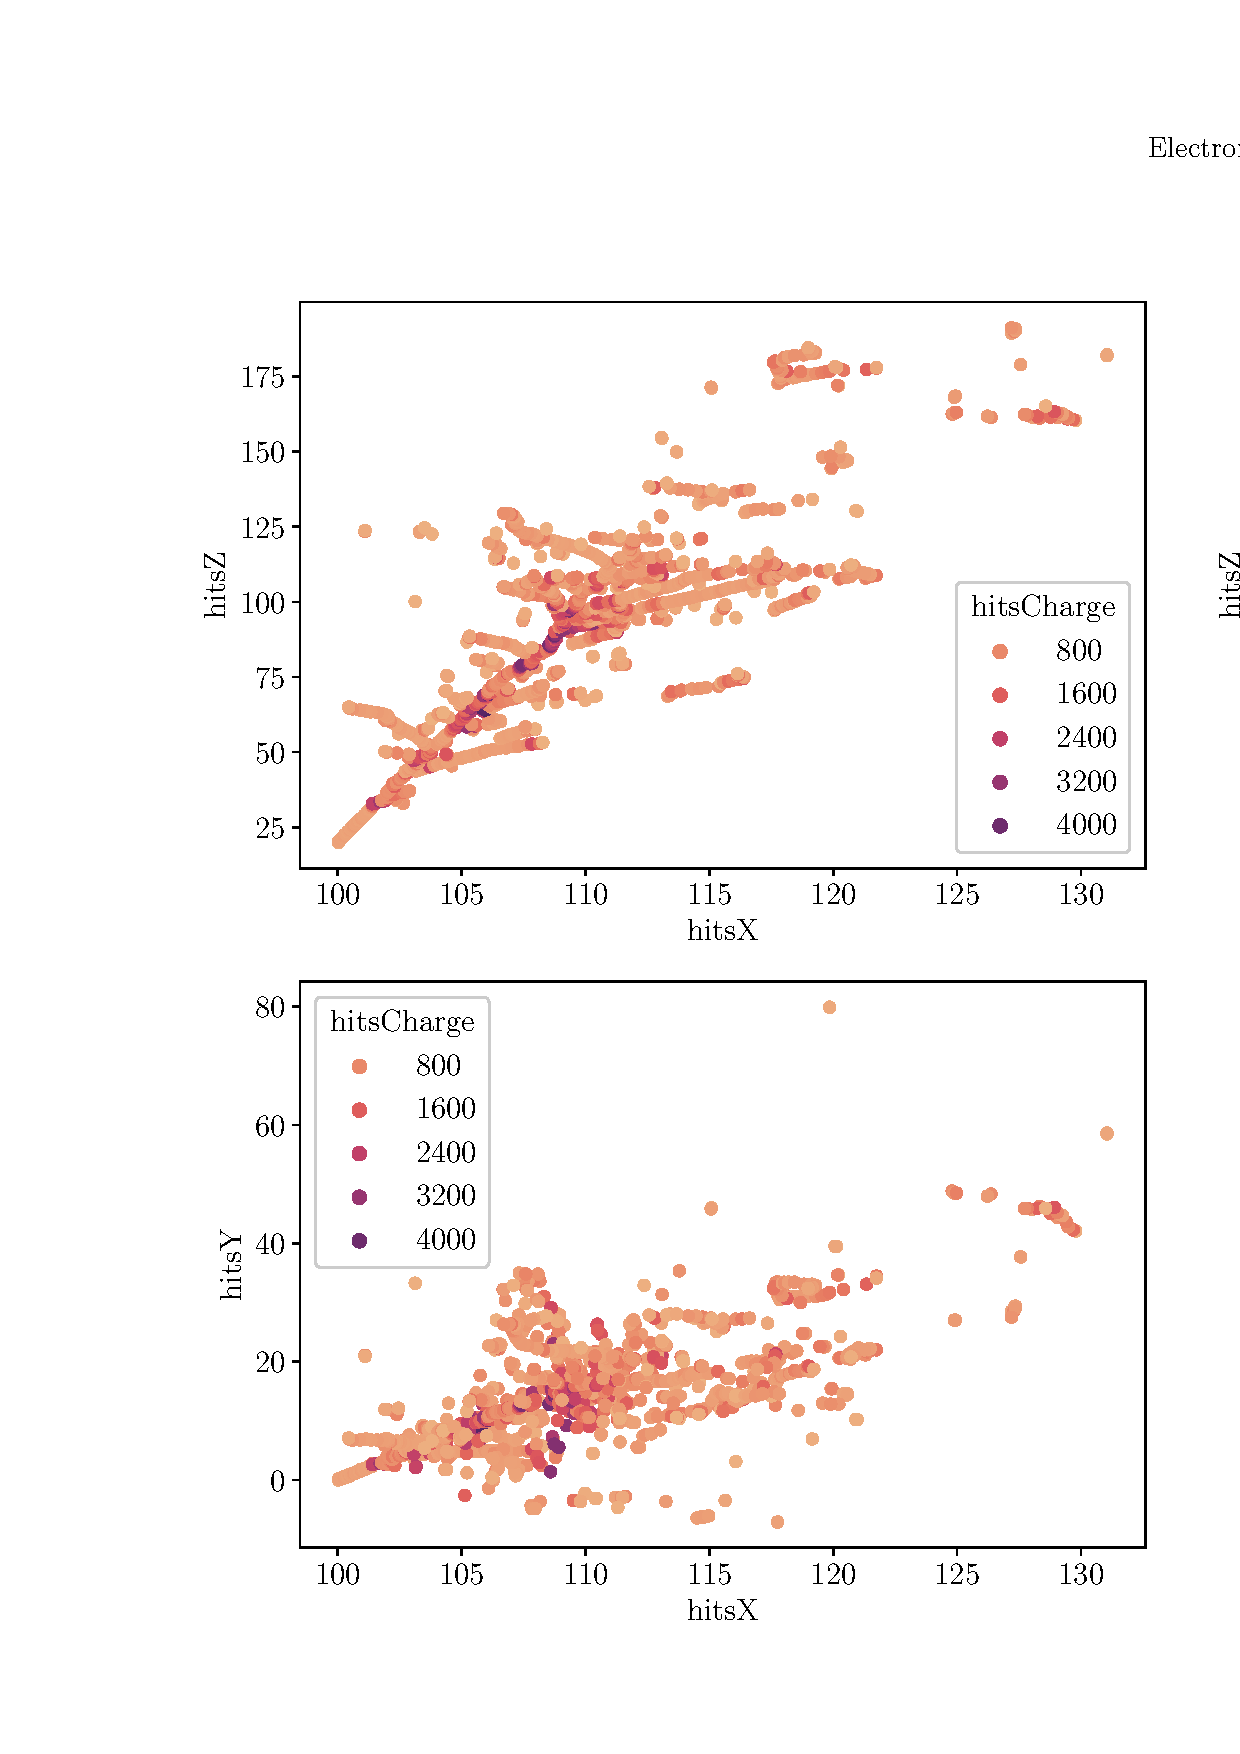
\includegraphics[scale=0.45, center]{comparación.pdf}
  \caption{Medidas simuladas de las trayectorias de las cascadas electromagnéticas. Se muestra una cascada originada por un electrón (izquierda) y otra originada por un fotón (derecha).}
  \label{fig:comparacion_cascadas}
\end{figure}

\subsection{Detector LArTPC}
\label{sec:lartpc}
Como se ha mencionado, los datos con los que vamos a trabajar proceden de simulaciones realizadas sobre un detector LArTPC, que se empleará en programas como SBN y DUNE. Veamos detalladamente cómo funciona y qué se mide en estos detectores \cite{sbnd}. En la Fig. \ref{fig:sensado} se muestra el esquema de funcionamiento de este detector.

\begin{figure}[h!]
  \centering
  \includegraphics[scale=0.65]{planos_sensado.PNG}
  \caption{Esquema de funcionamiento de un TPC \cite{sbnd}. La partículas cargadas en el interior del detector arrancan electrones que son dirigidos hacia los planos de hilos donde se recogen su energía, posición en dicho plano y tiempo de llegada. Con esta información junto con el instante de tiempo inicial del evento se reconstruye la trayectoria de las partículas cargadas.}
  \label{fig:sensado}
\end{figure}

Estos detectores consisten en un volumen de argón líquido (LAr), donde tiene lugar las interacciones, y una cámara de proyección temporal (TPC) que nos permite trazar la trayectoria de partículas cargadas. El hecho de que se use argón líquido se debe a que es un gas noble y, por tanto, es un gas inerte permitiéndonos mantener el medio lo más puro posible. Además, el Ar posee un potencial de ionización bajo, de manera que es sencillo que una partícula cargada ionice el medio dejando electrones libres. A todo esto se le añade que el Ar es un gas noble muy abundante \cite{lar_review}, que lo hace más accesible. 

El detector consiste en un criostato\footnote{Un criostato es un  dispositivo que nos permite mantener bajas temperaturas.} que contiene el argón y está dividido en dos partes por un plano que va a actuar como cátodo. Paralelo a este plano, en los extremos del criostato, vamos a tener planos de hilos que nos permiten registrar la señal dejada por los electrones liberados durante la ionización (ver Fig. \ref{fig:estructura_detector}). Cada plano consiste en tres planos de cables, que actúan como ánodo del circuito que van a recorrer los electrones libres. De esta forma, los detectores TPC son capaces de trazar las trayectorias de las partículas cargadas que se desplazan en su interior.

En la Fig. \ref{fig:estructura_detector} mostramos un esquema de la estructura del detector. En lo que sigue, vamos a tomar como eje $x$ la dirección del campo eléctrico, dirección en la que se van a desplazar los electrones libres y se denomina dirección de deriva. Como eje $z$, se considera el lado más largo del volumen del detector y esta será la dirección con la que entran los neutrinos. Finalmente, como eje $y$ tomaremos la dirección restante. Los planos de hilos se encuentran en los extremos del volumen, en el plano YZ.

\begin{figure}[h!]
  \centering
  \includegraphics[scale=0.45]{estructura_detector.PNG}
  \caption{Esquema de la estructura del detector LArTPC del programa SBN \cite{sbnd}. En el eje $x$, dirección de deriva, se observa el campo eléctrico aplicado para dirigir los electrones libres hacia los planos de hilos. El eje $z$ es el que contiene el lado más largo del detector y es la dirección con la que inciden los neutrinos. El eje $y$ es el eje restante. Vemos que perpendicular a la dirección de deriva tenemos un plano que parte el detector en dos regiones y actúa como cátodo. En los extremos se tienen los planos hilos que actúan como ánodos.}
  \label{fig:estructura_detector}
\end{figure}

Lo primero que vamos a mostrar es cómo, dada una partícula cargada, vamos a poder trazar su trayectoria. Cuando una partícula cargada con energía suficiente se mueve por el argón neutro puede darse que, por fuerza coulombiana, arranque  electrones ligados a los átomos de argón, generando electrones libres; de forma que se obtiene una traza de su recorrido. En la Fig. \ref{fig:sensado} se puede ver representado gráficamente este hecho.

Al aplicar un campo eléctrico, los electrones libres son dirigidos hacia los planos de hilos donde son recogidos emitiendo un pulso eléctrico. Hay muchos detectores que usan este principio, como puede ser un contador Geiger. Sin embargo, con el LArTPC se pretende reconstruir la trayectoria seguida por las partículas y para ello se hace lo siguiente. Por un lado, se utilizan fotodetectores para determinar el instante tiempo $t_0$ en el que comienza la trayectoria. En este instante es cuando el neutrino interacciona con el medio y, por tanto, el momento en el que comienza la trayectoria de las partículas que queremos estudiar. 

Cuando se origina la partícula cargada, esta se desplaza arrancando electrones que, con un campo eléctrico perpendicular al plano YZ, dirigimos hasta los planos de hilos en los extremos. Cada plano de hilos consiste en tres planos de cables que se pueden observar en la Fig. \ref{fig:sensado}. Estos planos son paralelos, pero los cables de cada plano tienen distintas orientaciones. La clave es que con dos de estos planos podemos determinar las coordenadas de los electrones libres en el plano YZ.

Para entender esto, simplifiquemos el problema. Supongamos que tenemos solo dos planos de hilos, uno vertical y otro horizontal, de manera que son perpendiculares entre sí, es decir, tenemos una rejilla. Cuando llegue uno de los electrones libres al plano se producirá una pulso eléctrico en uno de los cables del plano vertical y en uno del horizontal, por lo que sabiendo la posición de estos cables podemos determinar la posición del electrón en dicho plano. A estos pulsos les denominamos \textit{hits} y, además, recogemos información de la energía del electrón libre, ya que en el cable se recogerá una carga, proporcional a la energía, que es lo que se denomina carga del \textit{hit}. Adicionalmente, se mide el instante de llegada de los electrones al plano.

La situación real es que los planos no son horizontales y verticales, y el tercer plano está para deshacer ambigüedades que se pueden dar al realizar la reconstrucción. De forma que, los planos de hilos nos permiten obtener la posición en el plano YZ de los electrones que hayan sido arrancados por la partícula cargada. Lo que es lo mismo, obtenemos la trayectoria de dicha partícula proyectada en el plano YZ. Para obtener información de la dimensión restante lo que hacemos es usar $t_0$ y el tiempo de llegada de los electrones libre al plano, ya que al saber su velocidad de deriva en el medio, podemos obtener la distancia al plano YZ.

En resumen, inicialmente llega un neutrino, que interacciona con el Ar, obteniendo un protón y un electrón (recordemos que esta es una de las opciones posibles). Con los fotodetectores obtenemos el instante de tiempo en el que tiene lugar esta interacción. Al ser ambas partículas cargadas, vamos a tener un rastro de electrones libres por cada partícula que, debido al campo eléctrico en el eje $x$, se desplazan hacia el plano de hilos, obteniendo la proyección de cada trayectoria en el plano YZ. La información de la trayectoria en el eje $x$, la obtenemos usando el tiempo de origen, así como el tiempo en el que llegan los electrones al plano de hilos.

En definitiva, vamos a poder obtener la trayectoria completa de una partícula cargada, es decir, la región del espacio recorrida por la partícula. Los datos finales, tras procesar las señales, son las coordenadas de los \textit{hits} dejados por la partícula cargada. Estos datos se asemejan mucho a una imagen, que no es más que una matriz cuyos elementos representan los píxeles y su valor la intensidad. En nuestro caso, tenemos las coordenadas y la carga que lo podemos entender como la posición en la matriz y la intensidad, respectivamente.

Nosotros vamos a centrarnos en el estudio de las cascadas electromagnéticas que se van a producir en el interior del detector. Una de las situaciones que podemos tener es que el neutrino llegue, produzca un electrón y un protón, este electrón va a desplazarse por el medio creando electrones libres (y, por tanto, lo observamos) hasta que se desintegra generando un electrón y un fotón iniciándose la cascada electromagnética. La otra opción posible es que un fotón origine la cascada. Nuestro objetivo fundamental en este trabajo es conseguir distinguir ambos tipos de sucesos, ya que nosotros solo tenemos que contar las cascadas electromagnéticas producidas por electrones.

\section{Conceptos de computación}

En esta sección recogemos los conceptos relacionados con el Deep Learning y con la computación necesarios para comprender completamente este trabajo. En concreto, vamos a desarrollar los fundamentos del Deep Learning centrándonos en las redes convolucionales y haremos una breve descripción de qué es el MLOps.

% Mostraremos primero que es exactamente lo que vamos a estudiar, las cascadas electromagnéticas, y como es el detector que nos va a proporcionar los datos. También recogeremos información sobre algunos aspectos fundamentales en nuestro trabajo: el Deep Learning, técnicas MLOps y la explicabilidad en algoritmos de Machine Learning.

\subsection{Deep Learning}
\label{sec:dl}

El Deep Learning (DL) es un conjunto de técnicas y modelos que están dentro del ámbito del Machine Learning (ML), y que, en los últimos años, ha experimentado unos enormes avances en muchos problemas de ciencia de datos que se habían resistido a los métodos clásicos \cite{dl_nature}. Entre estos problemas se encuentran la clasificación de imágenes, donde el uso de redes neuronales convolucionales (CNN) se ha convertido en el estado del arte y ha conseguido obtener mejores resultados que los propios humanos en algunos problemas \cite{efficientnet}. Otros ejemplos son el procesamiento de lenguaje natural con los transformers o el reconocimiento del habla \cite{korean_dl}.

El DL tiene la ventaja de que es capaz de trabajar con los datos en bruto, de hecho, se define como el conjunto de modelos que son capaces de obtener las características directamente de los datos \cite{dl_book}. Estos rápidos avances se deben, en gran medida, a que se dispone de una gran cantidad de datos (gracias al desarrollo del Big Data) que pueden ser procesados automáticamente, así como de distintos avances tecnológicos \cite{korean_dl,dl_nature}. De hecho, los avances son tales que, con la combinación de modelos de DL, hemos pasado de ser capaces de clasificar imágenes a lograr generar imágenes nuevas dado un texto \cite{hier}. Otro gran avance son los modelos capaces de escribir código dadas las instrucciones de lo que se quiere realizar \cite{codex}, todo esto en un periodo de solo 10 años.

Con todo esto, vamos a ver los fundamentos necesarios para entender qué es una CNN, sus elementos, su complejidad y mostraremos algunos ejemplos de esta arquitectura de red neuronal. No profundizaremos demasiado, pero en esta sección se pretende mostrar qué es el DL y una CNN, y cuáles son sus principios básicos de funcionamiento. 

\subsubsection*{Fundamentos}

Las redes neuronales (NN) surgen con los perceptrones multicapa (MLP) que consisten en la composición de funciones paramétricas para formar una función más compleja. Este modelo está inspirado en el funcionamiento del cerebro, por analogía con las neuronas y sus activaciones. Esta representación se puede observar en la Fig. \ref{fig:mlp}, pero no es más que una manera de expresar una serie de operaciones matemáticas, donde los nodos representan las entradas y salidas de funciones, y los enlaces representan el valor de los coeficientes de la aplicación, que se denominan pesos. 
\begin{figure}[h!]
  \centering
  \includegraphics[scale=0.29]{MultiLayerPerceptron.png}
  \caption{Esquema de un modelo MLP con una capa de entrada, una capa oculta y una capa de salida \cite{mlp}.
  %  \href{https://creativecommons.org/licenses/by-sa/3.0/deed.en}{Creative Commons Attributions License (CC BY-SA)}.
  }
  \label{fig:mlp}
\end{figure}

De hecho, el paso de una capa a otra en un MLP no es más que una aplicación lineal:
\begin{equation}
  \label{eq:mlp_1}
  \mathbf{y} = W\mathbf{x},
\end{equation}
a la que se le aplica una función no lineal. Donde $\mathbf{x} \in \mathbb{R}^n $ es la entrada y son los nodos iniciales, $\mathbf{y} \in \mathbb{R}^m$ son los nodos de salida y la matriz $W$ se representa con los enlaces entre nodos. Destacar que las dimensiones de entrada y de salida no tienen por qué ser las mismas. Por otro lado, la función no lineal se aplica para que el modelo sea capaz de aprender relaciones más complejas. Hay muchas opciones, normalmente se usa la sigmoide o la RELU entre otras muchas y se suelen denominar funciones de activación \cite{dl_book}.

En la ecuación \ref{eq:mlp_1} lo que hemos mostrado es la función matemática de un MLP, donde solo tenemos una capa de entrada y otra de salida, y donde no se aplica ninguna función no lineal, este ejemplo equivale a un modelo de regresión. Se puede añadir más complejidad introduciendo más capas y estas funciones no lineales. Un ejemplo de la formulación de un MLP con una capa oculta es:
\begin{equation}
  \mathbf{z} = \sigma(W\mathbf{x}), \quad \mathbf{y} = \sigma(V\mathbf{z}),
\end{equation}
donde $\sigma$ representa la función sigmoide, $\mathbf{x}$ es el vector de entrada, $\mathbf{z}$ es el de salida de la capa inicial e $\mathbf{y}$ el vector de salida de la NN. Las matrices $W$ y $V$ definen las aplicaciones lineales y representan los enlaces entre capas.

Un detalle importante sobre estos modelos es que se puede demostrar que son aproximadores universales, es decir, que toda función puede aproximarse usando una NN \cite{aprox_1,aprox_2}, el problema surge con la cantidad de capas y neuronas necesarias, así como en el proceso de aprendizaje de los pesos correctos para representar dicha función.

El punto más importante de los modelos de DL es que son capaces de aprender las características necesarias para resolver el problema. Hasta entonces, si se quería estudiar una imagen, lo que se hacía era aplicar distintos algoritmos, como LBP, para obtener unas características concretas. Los algoritmos se diseñaban para resolver un problema concreto. El problema es que el diseño de estos algoritmos requiere de un esfuerzo muy grande y los resultados no son los mejores \cite{dl_nature}. Como ya hemos dicho, esto es posiblemente uno de los factores que han hecho posible que se tengan grandes avances, ya que no tenemos que perder tanto tiempo en la extracción de características \cite{dl_nature}. Estos modelos no solo agilizan el proceso, sino que además son capaces de detectar patrones que incluso los expertos no son capaces de visualizar.

Los MLP establecen las bases de todos los modelos actuales de Deep Learning. Con el tiempo, han ido surgiendo distintos tipos de NN, como las CNN, las RNN, los autoencoder o los transformers. En las MLP el paso de una capa a otra no es más que aplicar la función de activación tras realizar una aplicación lineal sobre un vector de entrada. Las distintas arquitecturas lo que hacen es cambiar esta representación y, por tanto, cambiar la función matemática aplicada sobre los datos de entrada. Cómo se definan las redes, influirá en los tipos de datos con los que la red podrá trabajar.

Otro aspecto importante es que las NN, por definición, no son más que la composición de distintas funciones donde cada función la podemos entender como una capa o incluso un conjunto de capas (la composición de funciones es una función). Esto simplifica la construcción de redes en el sentido conceptual porque, simplemente, basta con pensar en la combinación de distintos bloques y cómo interaccionan entre sí estos bloques. Por ejemplo, a las capas que forman un MLP se les denominan densas (todos los nodos están unidos) y un MLP no es más que el uso de varias de estas capas. En las CNN se usan lo que se denominan capas de convolución, que son un conjunto de capas que realizan la operación de convolución. Hay otros muchos bloques y el diseño de una NN consiste en la aplicación de sucesivos bloques que dependen del objetivo final que se tenga.

La dificultad reside en diseñar bloques que sirvan para el tipo de datos que se estén usando y en cómo combinar los bloques para obtener los resultados deseados, pero no en la construcción del modelo, una vez sabemos cuál es su forma.

\subsubsection*{CNN}

Las CNN son un tipo de NN donde la función matemática que se realiza es la de convolución. Antes de entrar en la parte matemática, mostremos la idea detrás de la capa de convolución. Para ello, supongamos que tenemos una imagen, que se representa como una matriz donde cada elemento describe a un píxel.

Sobre esta imagen podemos aplicar un filtro pequeño, por ejemplo, un bloque $3\times 3$ e ir recorriendo la imagen. Este filtro tendrá una forma dada por el valor de los píxeles del filtro. Por ejemplo, podemos definir un filtro que sea una línea horizontal, de manera que se tiene 1 en los píxeles que forman la línea y 0 para el resto de píxeles. Este filtro lo centramos en los distintos píxeles de la imagen y hacemos una operación que involucre al filtro y a los píxeles de la imagen que coincidan espacialmente con el filtro. Esta operación puede consistir únicamente en multiplicar elemento a elemento, los píxeles del filtro y de la imagen, y sumarlos. Es decir, sea una matriz $I$, la imagen, y una matriz $K$, el filtro, donde las dimensiones de $I$ son mayores que las de $K$. Lo que se hace es centrar la matriz $K$ en los distintos píxeles de $I$ y hacer un producto elemento a elemento, entre la matriz $K$ y la submatriz de $I$, y hacer la suma de los valores obtenidos. Si recogemos todos los resultados en una matriz, el resultado de aplicar el filtro sería otra matriz. Esto es lo que se conoce como operación de convolución, pero podemos cambiar la operación para realizar otros efectos sobre la imagen.

Veamos esto de manera formal. Sea $I$ una matriz de dimensiones $p\times q$ y $K$ una matriz de dimensiones $r\times s$ tal que $p>r$ y $q>s$. Por simplicidad, suponemos que $r$ y $s$ son impares. Definimos aplicar un filtro como:
\begin{equation}
  \label{ec:def_filtro}
  S_{i, j} = \sum_{n=1}^{r}\sum_{m=1}^{s}I_{i - \lfloor r/2 \rfloor + n, j - \lfloor s/2 \rfloor  + m}K_{n,m},
\end{equation}
con $i\in\{1,\dots, p -1 \}$ y $j\in\{1,\dots, q -1\}$. La matriz $S$ tiene dimensiones $p-1\times q-1$. Hay distintas definiciones según cómo tratemos los bordes de la imagen. Por ejemplo, podríamos considerar que cuando nos saliéramos de la imagen, se consideren los píxeles del otro extremo, de manera que la matriz resultante tendría las mismas dimensiones que la imagen original. También se puede aumentar la imagen introduciendo píxeles vacíos hasta poder aplicar el filtro en los bordes de la imagen inicial. Otro detalle que podemos destacar es que en la definición dada solo se contempla que el filtro se aplique centrándose en todos los píxeles posibles. Sin embargo, también se puede hacer de manera que el desplazamiento realizado al desplazar el filtro no sea un únicamente  píxel.

El uso de estos filtros nos permite determinar qué regiones de la imagen tienen unos patrones que nos pueden interesar. Con las CNN, la clave es que la red aprende los mejores filtros para realizar una tarea concreta. 

La operación que acabamos de describir se denomina convolución. Matemáticamente la convolución entre dos funciones $(x * w)(t)$ se puede escribir, en el caso de una dimensión, como:
\begin{equation}
  (x * w)(t):=\int_{-\infty}^{\infty} x(a) w(t-a) d a,
\end{equation}
donde $x$ y $w$ son funciones que dependen de una variable. En el ámbito del DL a $x$ se le denomina entrada y a $w$ el $kernel$ \cite{dl_book}. La expresión en el caso discreto quedaría como:
\begin{equation}
  (x * w)(t)=\sum_{a=-\infty}^{\infty} x[a] w[t-a].
  \end{equation}
Esta definición se puede generalizar para varias dimensiones, añadiendo tantas integrales como dimensiones. En el caso de las imágenes, tenemos que el espacio es discreto y que tenemos dos dimensiones, entonces, la operación de convolución quedaría:
\begin{equation}
  s[i, j]=(I * K)[i, j]=\sum_{m} \sum_{n} I[m, n] K[i-m, j-n],
\end{equation}
donde $I$ es una matriz de dimensiones $p\times q$, la entrada, y $K$ es una matriz de dimensiones $k\times l$, el $kernel$. Los límites de los sumatorios realmente serían de menos infinito a infinito, pero en nuestro caso, está determinado por las dimensiones de $K$ (podemos definir $K = 0$ si los índices superan las dimensiones). Notar la gran similitud con la ecuación \ref{ec:def_filtro}.

% Veamos esta expresión con el ejemplo que pusimos antes. $I$ es una matriz dada por la imagen, $K$ es el filtro y $s$ es la matriz final tras aplicar el filtro. Notar que la ecuación esta definida para los elementos de las matrices. La expresión anterior lo que nos dice es que el elemento $i$, $j$ de la matriz $s$ esta dado por hacer el producto elemento a elemento de la matriz $K$ con una parte de la matriz $I$ en un entorno del elemento $i$, $j$. Tras hacer el producto lo que se hace es sumar. Esto lo hacemos para todos los $i$, $j$ posibles y es lo que antes decíamos de aplicar el filtro a la imagen.

La capa de convolución consiste en aplicar el filtro y luego (en la mayoría de casos) aplicar una capa de reducción o \textit{pooling}, que consiste en reducir las dimensiones de la salida mediante la agregación de un grupo de píxeles. Por ejemplo, una imagen la podemos reducir si fragmentamos la imagen en bloques $2\times 2$ px y hacemos la media a estos bloques. Esta operación ayuda a que el resultado de la aplicación del filtro sea invariante a pequeños desplazamientos, que es fundamental a la hora de estudiar imágenes porque queremos que imágenes que se distinguan solo por desplazamientos, se clasifiquen igual (pensar que la imagen puede estar tomada desde puntos de vista distintos, pero contener el mismo objeto) \cite{dl_book}.

Estos son los elementos básicos de una CNN y es el punto de partida a la hora de construirlas. En resumen, hay muchas arquitecturas posibles para una NN donde cada una de estas arquitecturas tendrán unas características que hacen que sean útiles para un tipo de problema concreto. Las CNN son muy buenas a la hora de estudiar imágenes, ya que permiten estudiar regiones de la imagen y determinar qué elementos y patrones se tienen en la imagen, desde patrones muy simples, que se obtiene con las primeras capas de convolución, a patrones más complejos cuando aumentamos la complejidad del modelo.

\subsubsection*{Aprendizaje}

Hasta ahora hemos hablado de cómo es una NN. Sin embargo, no hemos entrado en cómo se determinan los pesos para que sean capaces de resolver un problema determinado. Sin entrar en mucho detalle, lo que se hace es emplear lo que se conoce como el descenso del gradiente \cite{gradient_descent} y la propragación hacia atrás, conocida por su término en inglés \textit{backpropagation} \cite{backpropa}.

El objetivo de un problema de ciencia de datos es, dados unos datos, usar un modelo que sea capaz de realizar una determinada tarea sobre estos con la intención de identificar patrones no triviales. En el caso del aprendizaje supervisado, se parte de que se tienen unas entradas de las cuales conocemos su clase/valor. Con estos valores se entrena el modelo para que realice la tarea concreta. Las NN hacen uso de los datos y sus etiquetas para determinar los pesos que mejor realizan la tarea concreta que se esté realizado. Las tareas clásicas en aprendizaje supervisado son la clasificación y la regresión \cite{dl_book}. En ambos problemas, tenemos un conjunto de instancias de las que tenemos distintas variables de entrada y una (o varias) variables de salida. La diferencia entre clasificación y regresión está en la variable de salida. La variable de salida en regresión toma valores en un rango continuo y su objetivo es predecir el valor de esta variable, dadas las variables de entrada. En clasificación, la variable de salida es discreta y al conjunto de valores posible se le suele denominar clase. El objetivo de la clasificación es determinar la clase de una instancia, dadas las variables de entrada.  

El descenso del gradiente consiste en definir una función pérdida que tome la clase dada por la red y la compare con la clase real. En el caso de que la red se equivoque, la salida de la función pérdida será mayor y será menor a medida que el modelo acierte la clase de las distintas instancias. Esta función va a depender de los pesos de la red, ya que son estos pesos los que determinan la clase que se asigna a la instancia. El descenso del gradiente consiste en obtener el gradiente de esta función pérdida con respecto a los parámetros de la red, obteniendo la dirección de crecimiento de la función. A continuación, se modifican los pesos en la dirección contraria para reducir el valor de la función pérdida y así mejorar los resultados.

Matemáticamente hablando, el problema consiste en la optimización de una función de varias variables, los pesos de red. Los pesos se inicializan de manera aleatoria, se calcula el gradiente y se cambian el valor de estos pesos en función del valor obtenido. El cambio se hace poco a poco y se regula con lo que se conoce como ritmo de aprendizaje ($lr$). Hay distintos algoritmos para este problema, como puede ser SGD o Adam \cite{sgd, adam}.

El proceso de aprendizaje suele realizarse dando un pequeño conjunto de datos, obteniendo el valor de la función pérdida para cada dato, promediando y, finalmente, ajustar los pesos calculando el gradiente. Esto se repite para todos las instancias y, normalmente, este procedimiento se hace varias veces con el mismo conjunto de datos, de manera que durante el aprendizaje el modelo estudia cada dato varias veces. Al conjunto de datos pequeños, se le conoce como \textit{batch size} ($bs$) y al número de veces que se recorre el conjunto de datos como número de épocas ($n_e$).

\subsubsection*{Elementos}

A modo de resumen final, vamos a recoger los distintos bloques que pueden formar una CNN. Un elemento necesario es el optimizador, algoritmo que realiza el descenso del gradiente, y el $lr$. En este punto, se construye la NN usando distintas capas. Las capas más simples son las que hemos ido mencionando. Una CNN muy simple la podemos construir como la aplicación de varias capas de convolución y tras esto, utilizar un MLP que clasifique los resultados.

Hemos mostrado los bloques más simples necesarios para construir una CNN, pero con el tiempo han ido surgiendo nuevos bloques y modificaciones sobre estos, con la idea de mejorar la optimización o los resultados. También hay distintas formas de unir todos estos elementos para construir la red. No vamos a entrar en estos bloques, pues ha habido una gran cantidad de avances en los últimos años y una revisión de estos elementos es un trabajo en sí. Los elementos y arquitecturas más complejos se irán describiendo a medida que nos vayan surgiendo la necesidad de estudiarlos.

\subsection{MLOps}

La resolución de un problema de ciencia de datos, es un proceso que puede llegar a ser muy complejo y depender de varias partes e incluso de varios equipos. De forma resumida, la resolución consiste en procesar los datos, analizarlos y entrenar un modelo. Una vez obtenido el modelo, este tiene que ponerse en funcionamiento y realizar la tarea para la que ha sido entrenado. En el momento que el proyecto crece, cada una de estas partes crece, llegando a un punto en el que cualquier modificación que se quiera realizar puede ralentizarse mucho debido a la complejidad del sistema.

El DevOps es un conjunto de prácticas para hacer el ciclo de desarrollo, implementación y ejecución de aplicaciones de forma eficiente \cite{mlops_nvidea}. MLOps, no es más que la aplicación de estas prácticas en una aplicación de Machine Learning. La filosofía de estos métodos de desarrollo es que los ciclos de versiones sean los más rápidos posibles, con la idea de aprender del funcionamiento de la aplicación y de la opinión de los usuarios, intentando automatizar lo máximo posible todas las etapas, minimizando los errores, mejorando la escalabilidad y manteniendo la calidad del código.

Veamos algunas de estas prácticas. El primer paso suele ser la integración y entrega continua, que consiste en probar de forma automática el software introducido, así como diseñar en torno a estas pruebas. Por otro lado, también se busca que el despliegue se realice de manera automática \cite{mlops_practical}. El empleo de sistemas de control de versiones como git es fundamental, al permitir tener un seguimiento de la evolución del proyecto, así como la colaboración entre personas. 

En MLOps, al DevOps, se le tiene que integrar la parte de ciencia de datos donde tenemos, por un lado, el procesamiento de estos datos y, por otro lado, el modelo final que es lo que nos interesa monitorizar y mejorar. Con estas técnicas se pretende automatizar el tratamiento de los datos, así como el despliegue y control sobre los modelos. En la Fig. \ref{fig:mlops} se muestra un esquema de un flujo de trabajo basado en MLOps, donde tenemos primero la parte de ciencia de datos en la que se tratan los datos y el modelo. Luego se tiene la parte de desarrollo donde, de manera automática, se verifica que todo funcione bien. A continuación, o bien se hace un despliegue, o bien se entrega el modelo al cliente, todo automáticamente. Tras el despliegue, entra en juego la parte de operaciones donde se hace uso de la aplicación y se aprende de su funcionamiento. Con esta información se modifican las etapas anteriores y se controla el correcto funcionamiento de los modelos.

\begin{figure}[h!]
  \centering
  \includegraphics[scale=0.50]{mlops.PNG}
  \caption{Esquema del flujo de trabajo basado en MLOps \cite{mlops_neal}. En el centro tenemos el flujo de desarrollo donde tenemos primero la planificación y la creación de la aplicación. Luego, entramos en el flujo de ML donde se procesan los datos y se crea el modelo. Con esto volvemos al flujo de desarrollo donde se verifica y despliega la aplicación. Finalmente, entra en juego el flujo de operación donde se monitoriza el modelo y la aplicación para que, dependiendo de su funcionamiento, se vuelva a comenzar el ciclo.}
  \label{fig:mlops}
\end{figure}

Nosotros en este trabajo nos vamos a centrar sobre todo en implementar muy bien una estructura automática para los datos y modelos, ya que nos va a permitir trabajar de manera mucho más ordenada y mantener un control del trabajo realizado y de los modelos obtenidos. En \cite{mlops_begin} se muestran tres niveles de implementación de MLOps: un primero, donde todo se hace de manera manual, un segundo, donde hay una estructura de flujo donde con el uso de cauces, se automatizan la mayoría de elementos y un tercero, donde se introduce la integración continua con el uso de test automatizados y el código se empaqueta y despliega automáticamente. Nosotros nos vamos a quedar en el segundo nivel donde tenemos un proceso completamente automático en el flujo de datos y del modelo, pero no vamos a entrar en el uso de test automáticos y despliegue automático, al ser un proceso más complejo, sobre todo para alguien sin experiencia previa.

\section{Estado del arte}

En física, los neutrinos estériles surgen como una explicación teórica, fuera del Modelo Estándar, de una serie de resultados anómalos en distintos detectores de neutrinos. En los detectores LSND \cite{lsnd} y MiniBooNE \cite{miniboo}, se ha observado un exceso del número de neutrinos esperados, compatibles con la existencia del cuarto neutrino \cite{sbnd}. Además, se han observado otras anomalías conocidas como la anomalía del reactor o la anomalía de Galio, que también podrían explicarse con la presencia del neutrino estéril. Los programas SBN y DUNE tienen como objetivo realizar experimentos de seguimiento que traten de confirmar que efectivamente se tienen esas anomalías \cite{sbnd, dune}. El detector microBooNE \cite{microboo} tenía un objetivo similar y ha publicado resultados recientemente, inconsistentes con los resultados de MiniBooNE \cite{micro_res}. Sin embargo, no dejan de ser unos resultados iniciales y siguen teniendo incertidumbres tales que no descartan completamente los resultados previos. Una de las incertidumbres principales proviene de la selección de los eventos que provienen de neutrinos y, por tanto, para reducir la incertidumbre, una de las cuestiones que hay que mejorar es la detección de cascadas electromagnéticas. 

En los últimos años, distintos laboratorios, como el CERN, han aplicado técnicas de DL \cite{ml_phy} con la idea de mejorar la capacidad de análisis de los datos que se obtienen. Modelos de DL se han usado para el seguimiento de partículas, la identificación de eventos, la identificación de \textit{Jets} o en simulaciones aplicando redes generativas \cite{dl_phy, dl_lhc, alb_1, alb_2}. De hecho, en microBooNE, un detector similar al nuestro, hace uso de las CNN para la clasificación de las cascadas \cite{ml_phy}.

Con respecto a la clasificación de imágenes, los mejores resultados en los últimos años vienen dados por CNN, con arquitecturas cada vez más complejas y más profundas. El rendimiento de estos modelos se suele evaluar en una competición anual con el conjunto de datos de ImageNet, que tiene muchas imágenes con muchas clases. Los ganadores de los últimos años han sido redes basadas en EfficientNet \cite{efficientnet}, que lo que hacen es introducir formas de escalar las redes (aumentar el número de capas y número de filtros) partiendo de un modelo base. Sin embargo, en los dos últimos años, los ganadores no han sido modelos basados en CNN, sino modelos que hacen uso de los transformers \cite{transformers} que son una nueva arquitectura de NN, que se han convertido en el estado del arte en procesamiento de lenguaje natural. Los modelos que aplican los transformers a la clasificación de imágenes se conocen como Visual Transformers (ViT) \cite{vit}, donde lo que hacen es proponer un modo de tratar las imágenes para que puedan ser empleadas por los transformers. ViT propone segmentar la imagen en bloques ($16\times 16$) y, manteniendo un orden, se pasan estos bloques a la red como si fueran una frase.

Otro aspecto fundamental en este trabajo es el uso del paradigma MLOps. Se puede definir como un conjunto de prácticas, conceptos y culturas de desarrollo con la intención de conseguir un rápido desarrollo de productos de Machine Learning y ponerlos en producción, tratando de solucionar el gran reto que supone la automatización y la puesta en funcionamiento de estos productos \cite{mlops_1}. Sin embargo, este término es muy reciente y está en pleno proceso de desarrollo, siendo aún muy ambiguo \cite{mlops_1}. No obstante, esta filosofía se fundamenta en el DevOps \cite{devops_1} aplicado a los modelos de  ML \cite{mlops_1}. Actualmente, se tienen distintas herramientas que nos facilitan la aplicación práctica de estas técnicas: MLFlow para el registro de modelos y despliegue automático de modelos \cite{mlflow}, Optuna para el ajuste de hiperparámetros \cite{optuna}, Snapper para facilitar la implementación en código de estas técnicas \cite{snapper, alb_3} o Amazon SageMaker como una plataforma en la nube con una gran batería de soluciones para facilitar el flujo de trabajo de un producto de ML \cite{sage}.

\chapter{Machine Learning aplicado a la clasificación de cascadas electromagnéticas}
\label{cap:3}

En este capítulo vamos a mostrar los datos y cómo los vamos a procesar para poder abordar el problema que se nos presenta, es lo que se conoce normalmente como ingeniería de los datos. Para ello, primero describiremos cuál es el problema y cuáles son los datos con los que partimos. 

Posteriormente, se mostrarán las distintas propuestas que hemos diseñado específicamente para la resolución de este problema, tanto en los modelos empleados como en el procesamiento de los datos. En este capítulo nos centraremos únicamente en enumerar las alternativas propuestas, en el Capítulo \ref{sec:arch} haremos un desarrollo detallado de su implementación y en el Capítulo \ref{sec:resultados} estudiaremos cuál de estas representaciones y modelos son los que mejores resultados consiguen.

En ningún momento vamos a entrar en el código desarrollado más allá de un esquema del flujo realizado\footnote{El código desarrollado está disponible en el repositorio: \url{https://github.com/aponce1509/tfm_}.}. No obstante, gran parte de este trabajo ha consistido en la implementación del flujo completo, pues se ha partido desde cero. Además, se ha dedicado una especial atención a hacer una implementación tratando de aplicar buenas prácticas de programación \cite{clean}, así como mantener una estructura de MLOps, teniendo en cuenta que, como físico, no se tenía una formación previa de cómo abordar de manera correcta un proyecto de desarrollo software. Todas estas prácticas son fundamentales a la hora de hacer el desarrollo de un proyecto de ML, tanto a modo de formación personal, como para que futuras personas puedan usar el código y continuar su desarrollo.


\section{Descripción del problema}

Como ya se ha mencionado, nuestro problema consiste en la clasificación de un tipo de evento que puede darse en un detector LArTPC, este evento se conoce como cascada electromagnética y puede originarse por un electrón o por un fotón. Nuestro objetivo es determinar si una cascada es de origen fotónico o electrónico. En la Sección \ref{sec:conceptos} se ha descrito de manera detallada cómo se producen dichas cascadas y cómo el detector transforma pulsos eléctricos en los datos con los que nosotros vamos a trabajar.

En nuestro caso, los datos están simplificados para contener únicamente cascadas electromagnéticas, por lo tanto, estos eventos son las trayectorias dejadas por estas cascadas en el interior del detector. Estos eventos los tenemos clasificados en función de qué tipo de partícula origina el evento.

% Lo primero que tenemos que entender es que para cada cascada vamos a tener muchos datos que nos van a permitir reconstruir tridimensionalmente la cascada. A cada una de las cascadas nos referiremos como eventos. Para cada uno de los eventos sabremos cual es la partícula que lo origina así como la energía de dicha partícula. Para la reconstrucción tenemos la posición tridimensional de donde se produce el \red{hit} y la carga depositada por dicho \red{hit}. 

Los datos que se nos han proporcionado consisten en datos tabulares etiquetados por el tipo de cascada. Tenemos 7 columnas, tres de ellas hacen referencia a un identificador del evento, a su energía en GeV\footnote{Un eV es una unidad de medida de energía que se define como la energía que tiene un electrón al aplicarle un campo eléctrico con una diferencia de potencial de 1V.} y al tipo de partícula, respectivamente\footnote{El Particle Data Group, con la idea de tener un identificador único y estandarizado para todas las partículas, asignó un número natural a cada una de las partículas para su identificación \cite{datagroup}. Las partículas que pueden originar los eventos que estamos estudiando son un electrón y un fotón, cuyos identificadores son el 11 y 22, respectivamente.}.  También se tienen otras tres columnas que describen la posición tridimensional del \textit{hit} dando las coordenadas $x$, $y$, $z$. La última columna recoge la cantidad de carga recogida del \textit{hit}, que es una magnitud proporcional a la energía depositada por la partícula cargada en ese punto de la trayectoria\footnote{Las unidades de la carga están dadas en tick $\cdot$ ADC, unidades que surgen del proceso de digitalización de la señal continua originada por los electrones libres en los planos de hilos del detector. La señal se digitaliza con una frecuencia de muestreo de \SI{5}{\micro s} que son los ticks y la cuantización de la señal se hace de manera que un electrón equivale a \SI[]{6.3e-3}{ADC}.}. 

Por otro lado, es importante indicar que en los datos no tenemos una única fila por evento, para cada evento tenemos varias filas que describen la trayectoria completa de la cascada.

Los datos con los que trabajamos provienen de simulaciones de Montecarlo que simulan con mucha exactitud el comportamiento real del detector. El uso de simulaciones supone una serie de ventajas. Por un lado, tenemos una gran cantidad de datos y se podrían obtener más en caso de ser necesario. Además, al tener control total de la simulación, tenemos información privilegiada, en el sentido de que es información que no se tiene en el detector real y se tiene que inferir. En concreto, disponemos del valor de la energía del evento, que realmente se tiene que obtener de distintas medidas en el detector. Por esto mismo, a la hora de hacer la clasificación no vamos a hacer uso de esta variable, pero sí la usaremos para validar el modelo y saber si nuestro modelo funciona correctamente para todos los rangos de energía.

Como hemos dicho, las trayectorias recogidas en los datos han sido filtradas para que solo contengan cascadas electromagnéticas. Realmente, un evento en el detector LArTPC está formado por la trayectoria de las distintas partículas que intervienen en una interacción. Por ejemplo, en la corriente cargada tendremos la traza dejada por el protón y el leptón. Por lo tanto, en el problema real sería necesario aplicar detección de objetos y quedarnos únicamente con la región que contenga a la cascadas, sin embargo, para esto necesitamos un buen clasificador, que es lo que se ha abordado en este trabajo. % En este trabajo no vamos a realizar la detección de objetos. 
En la Fig. \ref{fig:3d} se muestra una representación tridimensional de los datos tal cual se nos han proporcionado. En la Fig. \ref{fig:vistas} se muestran las tres vistas de esta misma trayectoria.
\begin{figure}[h!]
  \centering
  \includegraphics[scale=0.70, center]{3d_3.PNG}
  \caption{Representación tridimensional de una cascada electromagnética originada por un electrón con los datos en bruto. El color de los puntos viene dado en función de la carga del \textit{hit}. Se muestran también las proyecciones sobre el plano XZ y sobre el plano XY con colores fijos.}
  \label{fig:3d}
\end{figure}
\begin{figure}[h!]
  \centering
  \includegraphics[scale=0.65, center]{vistas_3.pdf}
  \caption{Representación de las tres vistas de una cascada electromagnética originada por un electrón con los datos en bruto. El color de los puntos viene dado en función de la carga del \textit{hit}.}
  \label{fig:vistas}
\end{figure}

Nuestro objetivo principal en este trabajo consiste en distinguir las cascadas originadas por los fotones de las producidas por los electrones y tenemos que ver cómo abordar este problema desde el punto de vista de la ciencia de datos. Este detector nos permite reconstruir los eventos como imágenes tridimensionales, por lo que podemos abordar este problema como un problema de clasificación de imágenes. Tratar los datos como imágenes es una selección que hacemos, ya que queremos ver cómo actúan los clasificadores de imágenes del estado del arte en este problema concreto. Esta decisión la hemos tomado, pues la forma natural representar los datos proporcionados por este detector es mediante imágenes\footnote{En la Sección \ref{sec:lartpc}, hemos descrito el funcionamiento del detector simulado y vemos cómo recoge la trayectoria de los eventos con la idea de visualizar las partículas como si estuvieran en una cámara de niebla, queremos ver las partículas y con este detector se pretende, entre otras cosas, obtener reconstrucciones tridimensionales de las trayectorias dejadas por las partículas.} y, además, nos permite entender y visualizar los eventos. Por otro lado, en \cite{auu} se ha llevado a cabo un enfoque con una representación numérica y nosotros queremos ver si una representación con imágenes mejora los resultados. % No obstante, hay otras alternativas y podríamos buscar otros enfoques no basados en imágenes y usar directamente los datos dados.

Las redes convolucionales son el estado del arte en clasificación de imágenes, por lo que todos los enfoques que vamos a desarrollar van a hacer uso de estas arquitecturas. Sin embargo, se pueden abordar mediante otros procedimientos, como puede ser hacer la clasificación mediante la definición de nuevas variables a partir de las imágenes o el uso de métodos clásicos de extracción de características. Estos enfoques son más clásicos en el sentido que no se hace uso del Deep Learning.

\section{Preprocesamiento de los datos}
\label{sec:des_trat}

Antes de entrar en los modelos que vamos a usar para hacer la clasificación, tenemos que ver cómo se tratan los datos iniciales para que podamos utilizar un modelo de aprendizaje. Lo primero que tenemos que hacer es pasar los datos a imágenes. En nuestro caso, al trabajar con imágenes tridimensionales, tendremos que trabajar con matrices con cuatro dimensiones, tres de posición y una para el canal de color. El color de la imagen lo asociaremos con la cantidad de carga depositada por el \textit{hit}, por lo que, en principio, trabajamos con imágenes en blanco y negro.

\subsection{Formas de representación}

Una vez que hemos construido las imágenes, vamos a plantear distintas formas de tratarlas que consideramos que pueden ayudar a la hora de discriminar los eventos. Estas son los que enumeramos a continuación:

\begin{itemize}
  \item Trabajar directamente con las imágenes tridimensionales. Las CNN no están limitadas a trabajar con imágenes bidimensionales, pues la operación de convolución se puede aplicar sobre matrices de cualquier dimensión.
  \item Trabajar con imágenes bidimensionales donde nos quedamos únicamente con una proyección. El problema con este enfoque es que se pierde información.
  \item Codificar la información perdida a la hora de hacer la proyección en el color de la imagen, de manera que mantenemos toda la información usando imágenes bidimensionales pero con tres canales de color.
  \item Entrenar distintos modelos para cada proyección y agregar los resultados. Podemos usar un ensemble o agregar las características obtenidas en los tres modelos.
\end{itemize}

Independientemente del modelo o enfoque empleado, es necesario pasar los datos tabulares a imágenes, pero surgen una serie de problemas al realizar esta conversión, en concreto, surge con la resolución de la imagen, pues si queremos mantener todos los \textit{hits} vamos a tener que imágenes muy grandes. Esto se debe a que la posición viene dada en centímetros y tenemos una precisión de varias décimas de milímetro, por lo que necesitaremos de muchos píxeles, ya que las dimensiones del detector SBND (el detector particular que hemos simulado en el estudio) son de $400\times400\times500$ \si{\cubic\cm}. Notar que la precisión del detector está relacionada con la resolución de la imagen, entendiendo resolución de la imagen como el número de píxeles que usamos para representar el volumen completo del detector. El problema surge si queremos mantener toda esta información, ya que necesitaríamos muchos píxeles y a más píxeles, mayor número de pesos vamos a tener en el modelo.
%  Otra cuestión a considerar es que tenemos un número considerable de filas en los datos tabulares, por lo que tenemos que tener esto en mente a la hora de hacer el cambio, ya que podemos tener problemas de memoria, de hecho, otro punto que se debería considerar en este problema es hacer uso de técnicas de Big Data para abordar el problema, no obstante, nosotros no vamos a entrar en ello al alejarnos del objetivo principal de este trabajo.

En el diseño de la implementación, es importante parametrizar las variables que influyen en el procesamiento de las imágenes, no solo para tener un seguimiento de las mismas, sino también para poder probar con distintas configuraciones. En concreto, es importante tener como parámetro la resolución final, así como el tamaño de la imagen, ya que son parámetros que pueden influir mucho en los resultados y la eficiencia del modelo.

\subsection{Transformación de los datos a imágenes}
\label{sec:trans_datos}

En esta sección se va a mostrar cómo vamos a implementar la generación de imágenes, que ha sido realizada desde cero. Se podría haber hecho uso de la librería $matplotlib$ simplificando mucho el problema, pero solo serviría en caso de trabajar con las proyecciones. Debido a que vamos a probar distintos enfoques, hemos realizado la implementación desde el principio. Además, los distintos procesamientos parten de la misma idea y modificar la represntación es simple en cuanto a implementación. Asimismo, de esta forma tenemos control total sobre las imágenes y todas van a compartir los parámetros.

Los datos proporcionados están en un sistema de referencia donde el eje $z$ va de \SI{0}{\cm} a \SI{500}{\cm} y los ejes $x$ e $y$ van de \SI{-200}{\cm} a \SI{200}{\cm}. Para regular la resolución y pasar los datos a una imagen, lo que vamos a hacer es aplicar un cambio de sistema de referencia, así como de unidades. Con estos cambios lo que pretendemos es regular la resolución, así como facilitar la creación de las imágenes.

\begin{figure}[h!]
  \centering
  \begin{tikzpicture}
    \draw[blue, ultra thick] (0,0) rectangle (4,4);
    \draw[black, ultra thick] (0, -1) -- (4, -1);
    \filldraw [black] (0,0) circle (2pt);
    \filldraw [black] (0,0.5) circle (2pt);
    \filldraw [black] (0,1) circle (2pt);
    \filldraw [black] (0,1.5) circle (2pt);
    \filldraw [black] (0,2) circle (2pt);
    \filldraw [black] (0,2.5) circle (2pt);
    \filldraw [black] (0,3) circle (2pt);
    \filldraw [black] (0,3.5) circle (2pt);
    \filldraw [black] (0,4) circle (2pt);
    \filldraw [black] (4,0) circle (2pt);
    \filldraw [black] (4,0.5) circle (2pt);
    \filldraw [black] (4,1) circle (2pt);
    \filldraw [black] (4,1.5) circle (2pt);
    \filldraw [black] (4,2) circle (2pt);
    \filldraw [black] (4,2.5) circle (2pt);
    \filldraw [black] (4,3) circle (2pt);
    \filldraw [black] (4,3.5) circle (2pt);
    \filldraw [black] (4,4) circle (2pt);
    \filldraw [black] (0, 0) circle (2pt);
    \filldraw [black] (0.5, 0) circle (2pt);
    \filldraw [black] (1, 0) circle (2pt);
    \filldraw [black] (1.5, 0) circle (2pt);
    \filldraw [black] (2, 0) circle (2pt);
    \filldraw [black] (2.5, 0) circle (2pt);
    \filldraw [black] (3, 0) circle (2pt);
    \filldraw [black] (3.5, 0) circle (2pt);
    \filldraw [black] (4, 0) circle (2pt);
    \filldraw [black] (0, 4) circle (2pt);
    \filldraw [black] (0.5, 4) circle (2pt);
    \filldraw [black] (1, 4) circle (2pt);
    \filldraw [black] (1.5, 4) circle (2pt);
    \filldraw [black] (2, 4) circle (2pt);
    \filldraw [black] (2.5, 4) circle (2pt);
    \filldraw [black] (3, 4) circle (2pt);
    \filldraw [black] (3.5, 4) circle (2pt);
    \filldraw [black] (4, 4) circle (2pt);
    \draw[black, ultra thick] (0, -1.2) -- (0, -0.8);
    \draw[black, ultra thick] (0.5, -1.1) -- (0.5, -0.9);
    \draw[black, ultra thick] (1, -1.1) -- (1.0, -0.9);
    \draw[black, ultra thick] (1.5, -1.1) -- (1.5, -0.9);
    \draw[black, ultra thick] (2.0, -1.1) -- (2.0, -0.9);
    \draw[black, ultra thick] (2.5, -1.1) -- (2.5, -0.9);
    \draw[black, ultra thick] (3.0, -1.1) -- (3.0, -0.9);
    \draw[black, ultra thick] (3.5, -1.1) -- (3.5, -0.9);
    \draw[black, ultra thick] (4, -1.2) -- (4, -0.8);
    \node[] at (2.0, -1.5) {$c_x = 8$};
    \draw[blue, ultra thick] (6,0) rectangle (10,4);
    \draw[black, ultra thick] (6, -1) -- (10, -1);
    \draw[black, ultra thick] (6, -1.2) -- (6, -0.8);
    \draw[black, ultra thick] (7, -1.1) -- (7.0, -0.9);
    \draw[black, ultra thick] (8.0, -1.1) -- (8.0, -0.9);
    \draw[black, ultra thick] (9.0, -1.1) -- (9.0, -0.9);
    \draw[black, ultra thick] (10, -1.2) -- (10, -0.8);
    \node[] at (8.0, -1.5) {$c_x = 4$};
    \filldraw [black] (6,0) circle (2pt);
    \filldraw [black] (6,1) circle (2pt);
    \filldraw [black] (6,2) circle (2pt);
    \filldraw [black] (6,3) circle (2pt);
    \filldraw [black] (6,4) circle (2pt);
    \filldraw [black] (10,0) circle (2pt);
    \filldraw [black] (10,1) circle (2pt);
    \filldraw [black] (10,2) circle (2pt);
    \filldraw [black] (10,3) circle (2pt);
    \filldraw [black] (10,4) circle (2pt);
    \filldraw [black] (7,0) circle (2pt);
    \filldraw [black] (8,0) circle (2pt);
    \filldraw [black] (9,0) circle (2pt);
    \filldraw [black] (7,4) circle (2pt);
    \filldraw [black] (8,4) circle (2pt);
    \filldraw [black] (9,4) circle (2pt);
    \filldraw [red] (7.2,0) circle (2pt);
  \end{tikzpicture}
  \caption{Esquema gráfico de la discretización de una trayectoria y de la influencia de resolución a la hora de describir una trayectoria. Se muestran como se describirían dos cuadrados cuando se toma una resolución de $c_x = 8$ y $c_x = 4$ asumiendo que los cuadrados ocupan todo el volumen posible. El parámetro $c_x$ denota el número de marcas necesario para el eje $x$ del volumen completo(ver discusión entorno a la Ec. \ref{eq:resolucion}).}
  \label{fig:esquema_regla}
\end{figure}

Para entender la idea que hay detrás de la creación de las imágenes pongamos el siguiente ejemplo. Supongamos que se tiene una regla que solo tiene marcados los centímetros. Si se emplea para medir el lado de un cuadrado que mide \SI[]{1.2}{cm}, al colocar la regla veríamos que el cuadrado acaba entre la marca con el 1 y con el 2, por lo que podemos decir que mide \si[]{1}{cm} con un cierto error, pues vemos que el cuadrado acaba más cerca del 1 que del 2, pero se pasa un poco (punto rojo de la Fig. \ref{fig:esquema_regla}). Con las transformaciones que planteamos, lo que hacemos es crear una regla donde el punto más pequeño lo colocamos en el cero y vamos variando el número de marcas ($c_x$) entre los extremos en función de la resolución deseada. De forma que si queremos aumentar la resolución, aumentamos el número de marcas y viceversa. El cambio de sistema de referencia lo realizamos para hacer que el mínimo sea 0 (colocamos la regla en el origen) y el cambio de unidades para fijar el valor del máximo al número de marcas de la regla ($c_x$). De esta forma, tenemos una regla entre los extremos del detector cuyas marcas corresponden a los píxeles de la imagen. En la Fig. \ref{fig:esquema_regla}, mostramos gráficamente cómo se describe un cuadrado, que lo podemos entender como el detector, para dos valores de $c_x$. Vemos cómo a mayor número de marcas, tenemos una mayor definición de su volumen, pero a cambio se necesita de una mayor cantidad de memoria para recoger toda la información. En la figura también se muestra un punto rojo que hace referencia a un posible \textit{hit} y nos permite visualizar que tras la transformación tenemos que aproximar estos puntos a las marcas.  

Otro modo de ver todo esto es mediante la conversión de una señal de analógico a digital, donde se tiene una señal continua y la queremos discretizar. Para realizar la conversión se establece una frecuencia de muestreo (marcas por centímetro). Si la frecuencia con la que se muestra la señal es alta, tendremos una mayor resolución de la señal, mientras que si establecemos una frecuencia menor, tendremos una peor resolución, ya que se toman menos puntos de la señal analógica, es decir, estamos usando menos marcas. El número total de marcas en un eje lo hemos denotado como $c_x$.

Para fijar ideas, supongamos que tenemos solo dos dimensiones y queremos acabar con imágenes $100\times100$ px. Para esto lo que hacemos es normalizar las posiciones al intervalo $\left[0, 100\right]$. Físicamente, es equivalente a realizar un cambio de referencia, de manera que el valor más paqueño en cada eje pase a ser cero, y luego hacer cambio de unidades para que el valor más grande en los eje pase a valer 100. Finalmente, redondeamos a un entero el resultado obtenido tras la transformación, obteniendo las marcas más cercanas a los puntos de la trayectoria que, además, nos sirve como índice para colocar el píxel en la matriz que representa a la imagen.

De manera formal, tenemos lo siguiente. Sea ${r} = (r_x, r_y, r_z)$ un punto cualquiera de la trayectoria de un evento cualquiera. Sean $t_{min} = (x_{min}, y_{min}, z_{min})$ y $t_{max} = (x_{max}, y_{max}, z_{max})$ tuplas que recogen los valores más pequeños y más grandes en cada eje, respectivamente. Estas tuplas se obtienen de todos los eventos de entrenamiento. Sea  $c = (c_x, c_y, c_z)$ una tupla con la resolución final de la imagen que contiene al detector completo. Las componentes de $c$ verifican:
\begin{equation}
  \label{eq:resolucion}
  c_x = c_y = \frac{5}{4}c_z,
\end{equation}
para que los tres ejes tengan las mismas unidades\footnote{Los valores de las posiciones en los tres ejes están dados en centímetros, pero los rangos son distintos. Por lo tanto, para mantener las dimensiones en los tres ejes tenemos que multiplicar por la misma constante en las tres dimensiones y en la Ec. \ref{ec:a} vemos cómo multiplicamos por $c / (t_{max} - t_{min})$ y, en consecuencia, depende del rango. El factor 5/4 surge de que en los ejes $x$ e $y$ se divide entre 400 y en el eje $z$ entre 500.}.

Lo primero que hacemos es aplicar el cambio de referencia (sumar a cada eje una constante a todos los puntos de todos los eventos) con la idea que el punto más pequeño esté en origen:
\begin{equation}
  {r}^\prime = {r} - t_{min}.
\end{equation}
Ahora, aplicamos el cambio de unidades (multiplicar a cada eje por una constante):
\begin{equation}
  \label{ec:a}
  {r}^{\prime\prime} = \frac{{r}^\prime}{t_{max} - t_{min}} \cdot c.
\end{equation}
Finalmente, redondeamos $r^{\prime\prime}$ a un entero. Aplicamos esta transformación a todos los eventos y a todos los puntos se obtiene, para cada evento, las posiciones dadas como números enteros cuyo mínimo es el cero y el máximo es $c$, obteniendo así los índices de los \textit{hits} en la imagen.

Las imágenes que obtenemos corresponden al detector completo, pero los eventos no ocupan todo el detector, por lo que debemos dar una parte de este volumen para evitar tener regiones vacías, es decir, nos quedamos con una ventana del detector. Además, estas ventanas tienen que ser de igual tamaño para todos los eventos, pero su posición sí depende del evento. Hay varias opciones para colocar la ventana:

\begin{itemize}
  \item En el ``centro de masa'' de la cascada que se obtiene usando la carga de los $hits$ del evento.
  \item En el comienzo de las cascadas, ya que sabemos que ahí es donde más diferencias hay entre los dos tipos de cascadas.
\end{itemize}

Nosotros hemos centrado las ventanas en el origen y el tamaño de esta ventana corresponde al tamaño de las imágenes con las que entrenaremos los modelos de clasificación. Este tamaño será otro parámetro que vamos a poder controlar a la hora de realizar la clasificación.

A la hora de colocar la ventana en el origen hay que tener en cuenta que, dependiendo de si el evento ocurre a la izquierda o a la derecha del cátodo, el evento se desarrolla en la dirección positiva del eje $x$ o en la dirección negativa. Lo que hemos hecho ha sido colocar el origen de la cascada en una de las esquinas inferiores de la imagen, pero la esquina se determina en función de la dirección de avance en el eje $x$. Para los otros ejes no se tiene este problema, pues en el eje $z$ se tiene que siempre se avanza en la dirección positiva y para el eje $y$ se tienen desplazamientos en ambas direcciones, por lo que colocamos el origen en un punto medio.

\subsection{Comentarios finales}

Como comentario final, es posible que, a la hora de hacer el paso de datos tabulares a imágenes, al estar cambiando la resolución, tengamos para el mismo punto del espacio dos valores distintos de carga (antes eran puntos distintos), por lo que tendremos que elegir un valor para estos puntos donde hay conflicto. Hay distintas opciones como puede ser tomar el máximo o la media, estas opciones también las introducimos como parámetros.
 
A modo de resumen, la creación de las imágenes consiste en primero obtener los máximos y mínimos de las coordenadas espaciales y de la carga. Con estos valores hacemos las transformaciones descritas obteniendo los índices para colocar los píxeles en la imagen. Tras la transformación, lo que se hace es utilizar alguna de las representaciones propuestas, como quitar uno de los ejes, quedarnos con la imagen tridimensional o hacer la codificación de la 3º dimensión en forma de color. Una vez se tienen los índices colocamos la ventana manteniendo siempre el origen de la cascada. En la Fig. \ref{fig:flujo_data} se muestra de forma esquemática el flujo que acabamos de describir.

\begin{figure}[h!]
  \centering
  \includegraphics[scale=0.4, center]{flujo2.pdf}
  \caption{Esquema del flujo realizado para realizar la transformación de los datos. Se parte de los datos simulados, que los dividimos en un conjunto de entrenamiento y otro de pruebas. Sobre el conjunto de entrenamiento obtenemos los máximos y mínimos de distintas variables necesarios para el procesamiento. Finalmente, creamos las imágenes, para ello discretizamos primero el detector y luego colocamos la ventana.}
  \label{fig:flujo_data}
\end{figure}

\section{Modelos propuestos}

 
Una vez se han procesado los datos y tenemos las imágenes, el siguiente paso es aplicar un modelo de clasificación. Vamos a hacer uso de las CNN que, aunque no son la única opción para la clasificación de imágenes, han mostrado muy buenos resultados. En esta sección simplemente vamos a enumerar los distintos modelos propuestos para realizar la clasificación:


\begin{itemize}
  \item Una CNN simple, con pocas capas que nos sirva de punto de partida.
  % \item \red{Una CNN compleja hecha por nosotros????}
  \item Una CNN más compleja, similar a la simple pero más densa y profundas es decir, con más filtros, neuronas, y capas ocultas.
  \item Hacer uso de arquitectura del estado del arte como pueden ser ResNet o EfficientNet. El entrenamiento lo hacemos usando los pesos aprendidos con el conjunto de datos de ImageNet reentrenando las últimas capas.
\end{itemize}

Hemos seguido un enfoque incremental donde hemos partido de modelos simples, como pueden ser redes basadas en la arquitectura LeNet, hasta usar redes más profundas y densas con la idea aumentar la complejidad hasta que no se observen mejoras en los resultados.

Uno de los problemas fundamentales que se tienen con el DL es que a medida que se tienen redes complejas, el número de pesos aumenta y esto hace que sea relativamente simple tener sobreajuste. De hecho, una de las limitaciones del DL es la gran cantidad de datos que se necesitan para entrenar los modelos. Este problema ha hecho que hayan surgido métodos de regulación, como el \textit{dropout}, que tratan de lidiar con el sobreajuste. El \textit{dropout} consiste en eliminar aleatoriamente un porcentaje de los enlaces entre dos capas y ha mostrado buenos resultados para reducir el sobreajuste \cite{dropout}.

Otras alternativas para reducir el sobreajuste consisten en introducir pequeñas modificaciones sobre las imágenes para aumentar la variabilidad de los datos, así como la cantidad de imágenes. Estas transformaciones suelen ser rotaciones, desplazamientos, cambios de brillo, reflexiones, etc. Esta técnica se conocen como \textit{data augmentation} y ha mostrado dar muy buenos resultados \cite{dataaug}. Sin embargo, no vamos a utilizarla, ya que trabajamos con simulaciones y podemos, hasta cierto punto, obtener más datos en caso de ser necesario. Además, transformaciones como rotaciones y reflexiones modifican la geometría del detector que es algo no deseado.

Otra opción, cuando se tienen pocos datos, es hacer uso de modelos que han sido entrenados con conjuntos de datos con muchas imágenes y muchas clases. Los pesos aprendidos, los modificamos ligeramente utilizado nuestro conjunto de datos \cite{transfer}. La idea detrás de este enfoque consiste en que estas redes han aprendido muchos patrones que se pueden aplicar en otras situaciones. Las CNN se pueden ver como dos grandes bloques: un extractor de características y un MLP para la clasificación. De forma que, al reentrenar modelos, podemos usar los dos bloques o mantener únicamente el extractor y usar un MLP completamente distinto. Por otro lado, los pesos que se modifican pueden ser todos, o simplemente los pesos de las capas más profundas, al ser las capas que contienen los patrones más complejos y, por tanto, son más específicos, que es posible que no funcionen bien para otro problema.

En definitiva, en este trabajo vamos a proponer varias representaciones de los datos, así como distintos modelos para la clasificación. En el Capítulo \ref{sec:arch} describiremos en detalle las arquitecturas usadas, así como las representaciones de los datos que hemos propuesto.

\section{Flujo de trabajo}

Sin entrar, todavía, en los detalles de la implementación, en esta sección se pretende mostrar, de forma esquemática, el flujo de trabajo del proceso de entrenamiento de los modelo, desde que se leen los datos hasta que se entrena el modelo. Este flujo está muy simplificado y pretende mostrar de forma general el diseño de esta parte del código. En la Fig. \ref{fig:flujo} se muestra el flujo mencionado.

\begin{figure}[h!]
  \centering
  \includegraphics[scale=0.40, center]{flujo1.pdf}
  \caption{Esquema del flujo de trabajo implementado para resolver el problema de clasificación de cascadas electromagnéticas. Los cuadrados son bloques de código mientras que las elipses representan datos, parámetros y modelos. En rojo se índica que forma parte del proceso de entrenamiento y validación mientras que en verde se recoge lo que se despliega tras el entrenamiento.}
  \label{fig:flujo}
\end{figure}

Inicialmente se parte de los datos, que consisten en 20000 cascadas, la mitad originada por electrones y la otra mitad originada por fotones. Lo primero que hacemos es separar el conjunto completo en un 90\% para entrenamiento y en un 10\% prueba, de manera que nos aseguramos que no se utiliza el conjunto de prueba en ningún momento. Además, es necesario fijar distintos parámetros que definen el tratamiento de los datos y el entrenamiento. En este punto, pasamos los datos tabulares a imágenes. Estas imágenes las volvemos a separar en un conjunto de entrenamiento y otro de validación (90\%-10\%). Con las imágenes de entrenamiento, entrenamos un modelo de clasificación definido en función de los parámetros establecidos y evaluamos el modelo usando el conjunto de validación. El modelo final es guardado junto con los parámetros para su uso futuro.

Este flujo mencionado está muy simplificado, veamos algunas cosas que son importantes mencionar. A la hora de entrenar el modelo, puesto que estamos usando redes neuronales, se dan varias vueltas por el conjunto de entrenamiento. En cada vuelta, validamos y continuamos entrenando hasta que no se observan mejoras en los resultados del conjunto de validación. Por otro lado, en el procesamiento de los datos necesitamos obtener el mínimo y máximo de varias magnitudes, por lo que, al aprenderlas con el conjunto de entrenamiento, estas tienen que guardarse con el modelo para poder procesar imágenes futuras.

Hay que tener en cuenta que tenemos un conjunto de parámetros que vamos a tener que explorar para mejorar los resultados. Para esto, utilizamos la librería Optuna \cite{optuna} que nos permite realizar esta búsqueda de una forma más eficiente que haciendo una búsqueda de rejilla, al tratar de optimizar una función objetivo. La implementación consiste en una pequeña modificación del flujo, donde hay que definir una nueva función objetivo y en función de los resultados obtenidos tras la validación se modifican los parámetros iterativamente. 

En la Fig. \ref{fig:flujo_code} mostramos, en código, el flujo de entrenamiento, es decir, todo menos la evaluación del modelo sobre el conjunto de prueba, que se hace aparte. Lo primero que hacemos es fijar la semilla aleatoria y configurar MLFlow fijando el lugar donde se guardan los modelos y el nombre del experimento. Luego obtenemos los datos y los elementos necesarios para el modelo y su optimización. Finalmente, entrenamos y guardamos los resultados en MLFlow. Este es el cauce principal y él más simple. Tenemos otros cauces, en los que no vamos entrar, que implementan la búsqueda de hiperparámetros o el estudio de los modelos usando en los distintos conjuntos de datos entre otros. Todo el código está disponible en \href{https://github.com/aponce1509/tfm_}{GitHub}\footnote{\url{https://github.com/aponce1509/tfm_}}.

Por otro lado, como ya se mencionó, hemos hecho uso de técnicas de MLOps que no se recogen completamente en el flujo descrito. Las prácticas MLOps que hemos llevado a cabo se pueden resumir en:
\begin{itemize}
  \item Encapsulación de las distintas partes del flujo de manera que cualquier modificación realizada no afecte al flujo completo, teniendo así un sistema de cauces que nos permite un desarrollo cómodo. En el código observamos cómo, por un lado se obtienen los conjuntos de entrenamiento, y por otro lado, se entrena el modelo. Esta filosofía se ha mantenido durante todo el desarrollo, pues simplifica mucho el diseño y la implementación de nuevas funcionalidades. 
  \item Todos los modelos entrenados, junto con sus resultados y parámetros, han sido guardados haciendo uso de MLFlow. Una herramienta que facilita mucho tanto el despliegue como el seguimiento de los resultados.
  \item Con respecto al despliegue, se ha construido un flujo que parta de datos nuevos (en nuestro caso el conjunto de prueba) y el identificador del modelo aprendido, y clasifique los datos. También se han añadido funciones que nos permiten estudiar los modelos, así como sus resultados.
  \item Aunque el trabajo no ha sido desarrollado por un equipo, donde es obligatorio establecer un repositorio central para recoger las métricas y modelos, hemos tenido que establecerlo y configurar MLFlow al trabajar con clusters de ordenadores, que han sido necesarios para realizar todas las pruebas llevadas a cabo en este trabajo.
  \item Se ha hecho la implementación para que al efectuar el entrenamiento, solo sea necesario indicar los parámetros de los modelos y del preprocesamiento. Para la evaluación de nuevos datos solo se requiere indicar un identificador del modelo que se quiere usar.
\end{itemize} 

\begin{figure}[h!]
  \centering
  \includegraphics[scale=0.3]{basic_pipe.png}
  \caption{Función con el flujo de entrenamiento del modelo. Hemos quitado los comentarios para mostrar el código de manera más clara.}
  \label{fig:flujo_code}
\end{figure}

\newpage
\chapter{Análisis de los datos}
\label{cap:4}

En este capítulo vamos a analizar los datos con la idea de poder entenderlos mejor y justificar las decisiones tomadas sobre cómo procesar los datos y cómo crear las imágenes según la metodología comentada en el capítulo anterior. Asimismo, nos permite mostrar el efecto de la resolución y el tamaño de las imágenes en cuanto a qué cantidad de cascada se pierde. En concreto, nos centraremos en estudiar el rango y distribución de las distintas variables.

Como ya se ha mencionado, una de las variables que tenemos para cada evento es la energía de la partícula que origina la cascada. Recordemos que esta variable se tiene gracias a que trabajamos con simulaciones y solo se usará para hacer el estudio de los resultados obtenidos. En la Fig. \ref{fig:hist_energia} se muestra un histograma de la distribución en energía donde vemos que se tiene una distribución uniforme, es decir, no hay rangos de energía donde se tengan más eventos. Los datos se han generado con esta distribución intencionadamente porque nos permite entrenar con la misma cantidad de eventos todo el espectro de energías. La dependencia con la energía es crucial para investigar la física que ocurre en las cascadas, por lo que será necesario evaluar las métricas de los modelos en función de la energía para estudiar cómo afectan al rendimiento de los modelos de clasificación.
% En la realidad no se espera que los datos tomados por el detector real sigan esta distribución 

\begin{figure}[h!]
  \centering
  \includegraphics[scale=0.85]{hist_en.pdf}
  \caption{Histograma de la energía de los distintos eventos.}
  \label{fig:hist_energia}
\end{figure}

Otra variable que resulta importante comprender es la posición. En concreto, nos interesa saber el volumen del detector ocupado por los eventos, ya que nos permite entender el efecto que tienen la resolución y el tamaño de la ventana en la imagen. Para obtener el volumen agrupamos los datos por eventos y calculamos el rango en los distintos ejes para cada evento. Es decir, para cada evento restamos el máximo y el mínimo en cada eje, obteniendo el rango para los tres ejes y para cada evento. A estas nuevas variables las vamos a denominar simplemente rangos. En la Fig. \ref{fig:hist_rango} se muestran los histogramas para estas nuevas variables y en la Tabla \ref{tab:cuartiles_rango} mostramos los cuartiles.

\begin{figure}[h!]
  \centering
  \includegraphics[scale=0.85]{hist_rango.pdf}
  \caption{Histograma de los rangos. Los rangos hacen referencia a la distancia entre el \textit{hit} que ocurre en el valor más pequeño y él que ocurre en el valor más grande. Se obtienen para los tres ejes espaciales y para cada evento.}
  \label{fig:hist_rango}
\end{figure}

\begin{table}[h!]
  \centering
  \begin{tabular}{|c|c|c|c|}
  \hline
           &  hitsX (\si{\cm}) &  hitsY (\si{\cm}) &  hitsZ (\si{cm}) \\ \hline
  min      &        0.04 &        0.00 &        0.40 \\ \hline
  25\%     &       31.26 &       48.79 &      111.90 \\ \hline
  50\%     &       47.47 &       71.12 &      140.50 \\ \hline
  75\%     &       72.23 &       98.97 &      170.15 \\ \hline
  max      &      263.51 &      312.29 &      429.40 \\ \hline
\end{tabular}
\caption{Cuartiles de los rangos que alcanzan las cascadas en los distintos eventos y ejes.}
\label{tab:cuartiles_rango}
\end{table}

Antes de entrar a discutir estas gráficas, recordemos que el parámetro $c$ nos permite regular la resolución con la que se describe el volumen completo del detector. Supongamos que queremos tener una precisión de \SI{0.1}{\cm}, es decir, construir una imagen donde la distancia entre dos píxeles consecutivos equivalga a \SI{0.1}{\cm}. En este caso, teniendo en cuenta las dimensiones del detector: $x \in [-200, 200]$ \si{\cm}, $y \in [-200, 200]$ \si{\cm} y $z \in [0, 500]$ \si{\cm} el valor de $c$ tendría que ser $(4000, 4000, 5000)$ \si{px}. Básicamente, lo que tenemos que hacer es fijar una precisión y dividir el rango de los ejes por esta precisión. Este valor de $c$ es la resolución y significa que representamos el volumen completo del detector con una malla de $4000\times 4000\times 5000$ \si{px}. Un evento dentro de este volumen ocupara solo una parte y lo que hacemos es coger una ventana del volumen completo.

Si nos queremos asegurar de que no se pierde nada de información al tomar la ventana, tenemos que ver cuál es el rango máximo que puede darse en un evento, que lo podemos ver en la Tabla \ref{tab:cuartiles_rango}. En el caso de que la precisión sea de \SI{0.1}{\cm}, tendríamos que usar imágenes de $2636\times 3123\times 4294$ \si{px} que son imágenes muy grandes. Sin embargo, si nos conformamos con mantener la información completa del 75\% de los eventos, el tamaño de la ventana sería de $723\times 990\times 1701$ \si{px} que siguen siendo imágenes muy grandes, pero son considerablemente más pequeñas. A la hora de entrenar los modelos, vamos a tener que jugar con los parámetros de resolución y de tamaño de la ventana para regular la cantidad de información que se mantiene al crear las imágenes. Es importante mencionar que la información que se pierde es, en su mayoría, la parte final de la cascada\footnote{Debido a la geometría del problema, tras originarse las cascadas, estas se desarrollan de menor $z$ a mayor $z$ y en el eje $x$ depende de si ocurre a la derecha o la izquierda del cátodo porque siempre se dirigen hacia el ánodo (recordar Fig. \ref{fig:sensado} y \ref{fig:estructura_detector}). Al generar las imágenes, las centramos en el origen colocando el origen en una esquina, de manera que se recoja la dirección de avance. Sin embargo, puede darse que, en algunas ocasiones, las partículas emitidas durante la interacción se dirijan en la dirección contraria, dando situaciones en las que se puede perder un poco de información no correspondiente al final de la cascada.}, mientras que el origen se mantiene siempre. Lo hacemos de esta forma, ya que en origen de la cascada es donde se tienen las principales diferencias entre las cascadas electromagnéticas que queremos clasificar. En la Fig. \ref{fig:varias_resoluciones} se muestra el mismo evento para distintos valores de resolución, donde vemos como a para valores muy bajos tenemos toda la cascada pero con muy poca definición de la cascada. Sin embargo, a medida que se aumenta la resolución, vemos cómo se va definiendo la cascada, pero vamos perdiendo información. El tamaño de las imágenes mostradas es de $128\times128$ px.

\begin{figure}[h!]
  \centering
  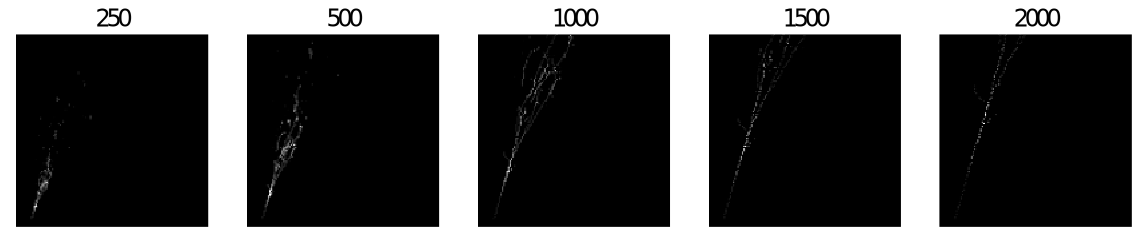
\includegraphics[scale=0.65, center]{varias_resoluciones.pdf}
  \caption{Mismos eventos representados para distintas resoluciones (número de píxeles que describen el detector completo). El tamaño de las imágenes es de $128\times128$ px.}
  \label{fig:varias_resoluciones}
\end{figure}


Por último, vamos a estudiar los \textit{hits} y su energía. La cantidad de \textit{hits} que se tienen por evento depende de la energía del suceso. En la Fig. \ref{fig:scatter_n_e} se muestra la relación que hay entre el número de \textit{hits} de un evento y la energía del mismo donde observamos que hay una tendencia positiva, es decir, a más energía mayor número de hits. El problema se tiene sobre todo cuando se tienen pocos \textit{hits}. Hay ocasiones donde un evento está dado por entre 5 y 10 \textit{hits}, siendo el evento con menos \textit{hits} uno que viene dado por 3 \textit{hits}. Es interesante ver cómo se comportan nuestros modelos en rangos de energía bajos.

\begin{figure}[h!]
  \centering
  \includegraphics[scale=0.85]{scatter_n_e.pdf}
  \caption{Diagrama de dispersión donde se muestra la relación entre el número de \textit{hits} de un evento y la energía. El número mínimo de $hits$ en un evento es de 3 \textit{hits}.}
  \label{fig:scatter_n_e}
\end{figure}


En la Fig. \ref{fig:hist_charge} se muestra la distribución de la carga de los \textit{hits}. Se muestran dos distribuciones, una donde lo que hemos hecho ha sido normalizar dividiendo por el valor máximo de la carga, así como la distribución tras aplicar una transformación logarítmica. En esta gráfica vemos que parece que, a simple vista, la distribución de los \textit{hits} sigue una distribución exponencial, donde tenemos que la mayoría de \textit{hits} depositan poca carga, mientras que muy pocos tienen valores de carga mayores. Notar que, al haber dividido por el máximo, hay al menos un \textit{hit} con valor 1 en la carga normalizada. Sin embargo, vemos que tras aplicar la transformación se pierde esta distribución exponencial y tenemos una distribución que en ciertas ocasiones puede ser deseable al estar los \textit{hits} más distribuidos.

\begin{figure}[h!]
  \centering
  \includegraphics[scale=0.85]{hist_charge.pdf}
  \caption{Histogramas de la carga de los \textit{hits} que se observan en los distintos eventos. Se muestran los datos sin aplicar ninguna transformación y los datos tras aplicar una transformación logarítmica.}
  \label{fig:hist_charge}
\end{figure}


Este comportamiento es importante tenerlo en mente, ya que en algunos casos puede que los \textit{hits} más energéticos tengan valores tan grandes que, en comparación, los menos energéticos no tengan nada de importancia. Una forma de solucionar este problema es aplicar la transformación logarítmica mostrada. A la hora de entrenar los modelos, vamos a tener que considerar esta transformación porque pueden llevar a una mejora de los resultados. Además, esta distribución exponencial puede dar lugar a que, al tener mucha diferencia entre los valores donde se encuentran la mayoría de \textit{hits} y el máximo, se tengan las imágenes prácticamente negras.

Otro factor que es interesante observar en la carga, es su distribución en función del tiempo, ya que es conocido que al comienzo del evento se deben observar valores más altos para la carga. Aunque no se dispone de la variable tiempo, se puede inferir al tener los datos ordenados temporalmente. En la Fig. \ref{fig:hist_charge_t} se muestra un histograma bidimensional donde en el eje $x$ se tiene el tiempo y en el eje $y$ se muestra el logaritmo de la carga. Hay que tener en cuenta que el tiempo se ha normalizado para cada evento, es decir, un valor de tiempo igual a 0 equivale al comienzo del evento y un valor de 1 equivale al final. De igual forma, la carga se ha normalizado usando el valor máximo observado en el conjunto de entrenamiento. Vemos que la distribución en el tiempo es prácticamente constante, salvo al principio, donde observamos \textit{hits} con energías superiores.

\begin{figure}[h!]
  \centering
  \includegraphics[scale=0.85]{hist_charge_time.pdf}
  \caption{Histogramas bidimensional donde se muestra la distribución de hits en función de la carga y el tiempo. Ambas variables las hemos normalizado para que tomen valores entre cero y uno.}
  \label{fig:hist_charge_t}
\end{figure}


\chapter{Desarrollo de los modelos para la clasificación}
\label{sec:arch}

En este capítulo vamos a recoger y desarrollar todas las propuestas que se plantean en este trabajo en lo referente a la representación de los datos y la construcción del modelo de clasificación. La construcción de las imágenes datos ha sido discutida en los Capítulos \ref{cap:3} y \ref{cap:4}. Primero haremos una descripción detallada de las distintas representaciones diseñadas necesarias para que los modelos entiendan los datos. Asimismo, mostraremos las arquitecturas de los distintos modelos que vamos a emplear. También, se muestran las métricas que emplearemos para realizar el entrenamiento y validar el modelo. Finalmente, se listarán todos los parámetros que se tienen en el código desarrollado y permiten modificar el preprocesamiento de los datos y el entrenamiento del modelo.

\section{Representaciones de los datos}

Como ya hemos visto, hay muchas opciones a la hora de crear las imágenes desde los datos tabulares. En esta sección vamos a describir las distintas representaciones que hemos propuesto. Todas estas representaciones parten de hacer el cambio de unidades y de sistema de referencia que se ha descrito en la Sección \ref{sec:des_trat}. En general, todas las propuestas buscan una forma de tratar con la tercera dimensión espacial, que no se puede recoger en una imagen típica. 

\subsection*{Representación tridimensional}

Una forma de abordar el problema es quedarnos con toda la información y no descartar ninguna dimensión porque la operación de convolución no está limitada a trabajar con dos dimensiones espaciales. Esta representación es conceptualmente muy simple, pero surgen una serie de problemas relacionados con el tamaño de las imágenes y que no se tienen modelos complejos previamente entrenados, como sí ocurre para las imágenes bidimensionales. En la Fig. \ref{fig:proy_3d} se muestra gráficamente el resultado de usar esta representación sobre uno de los eventos.

\begin{figure}[h!]
  \centering
  \includegraphics[scale=0.85, center]{rep_3d.PNG}
  \caption{Evento procesado manteniendo las tres dimensiones espaciales. Se ha tomado una resolución $c_x$ de 500 px y tamaño $128\times128\times128$ px.}
  \label{fig:proy_3d}
\end{figure}

\subsection*{Representación bidimensional, una proyección}

Otra opción es proyectar la imagen tridimensional y quedarnos con una de las vistas obteniendo una imagen bidimensional con un solo canal de color. Si recordamos, el eje $x$ es el eje de deriva, el haz de neutrinos está dirigido en la dirección del eje $z$ (el momento de la partícula tiene la dirección del eje $z$) y eje $y$ simplemente la altura con la que llega el neutrino al detector.

La implementación de esta representación consiste en quitar la columna del eje que se quiera proyectar. Notar que, entonces, puede darse que se tengan $hits$ que tengan la misma posición tras realizar la proyección. Cuando se tienen conflictos, nos quedamos con la media o con el máximo de la carga. Por lo demás, se aplican los cambios de unidades y de sistema de referencia que se describieron en la Sección \ref{sec:trans_datos}. En la Fig. \ref{fig:varias_proyecciones} se muestra gráficamente un evento que ha sido obtenido usando los datos tabulares directamente, así como la imagen con la representación que se acaba de describir. Los parámetros que hemos utilizado para la creación de la imagen procesada es de $c_x = 1000$ px para la resolución, un tamaño de ventana de $128\times 128$ px y no se ha aplicado la transformación logarítmica. En la Fig. \ref{fig:muchas_proyecciones} se muestran varios eventos con esta representación, tanto para cascadas electrónicas como fotónicas.

\begin{figure}[h!]
  \centering
  \includegraphics[scale=0.85, center]{ambas_pro.pdf}
  \caption{En la izquierda se muestra un evento proyectado obtenido de los datos tabulares directamente sin hacer uso del procesamiento que presentamos. En la derecha se muestra la imagen procesada con una resolución de 1000 px y tamaño $128\times128$ px.}
  \label{fig:varias_proyecciones}
\end{figure}

\begin{figure}[h!]
  \centering
  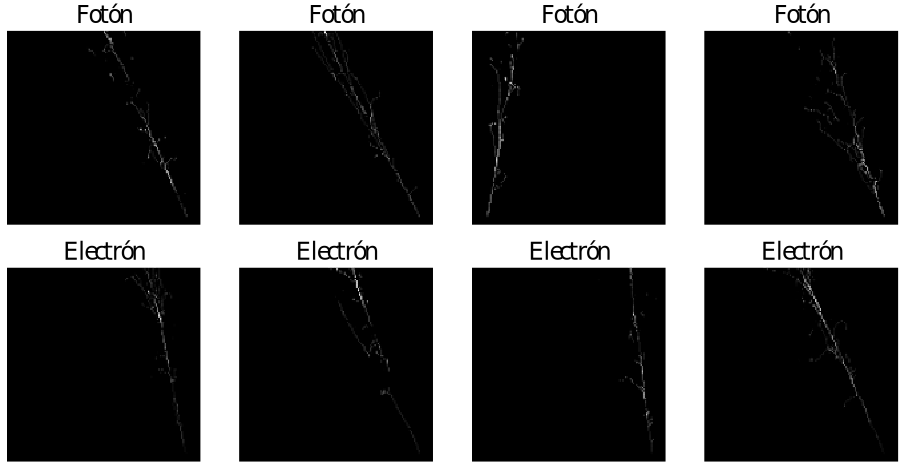
\includegraphics[scale=0.75, center]{varias_proyecciones.pdf}
  \caption{Imágenes obtenidas tras procesar y quedarnos con la proyecciones en el eje $y$ para distintos eventos. Las imágenes han sido procesadas con una resolución de 1000 px y tamaño $128\times128$ px.}
  \label{fig:muchas_proyecciones}
\end{figure}

\subsection*{Representación bidimensional, codificación del color}

Independientemente del eje que proyectemos vamos a perder información, ya que las cascadas se desarrollan en las tres dimensiones espaciales, incluso al proyectar el eje $y$ que es con el que se pierde menos información. Una forma de mantener esta información es codificar de alguna forma el color de la imagen para que contenga esta información.

Hasta ahora, hemos estado trabajando con imágenes en blanco y negro donde solo se tiene un canal. En el caso de trabajar con imágenes que tengan color es necesario trabajar con los tres canales de color. Hay distintos espacios para recoger el color de una imagen, el más común es el RGB donde los canales recogen la cantidad de rojo, verde y azul en la imagen. Hay otros muchos espacios y en función de lo que se quiera hacer con la imagen será más adecuado usar uno u otro. Nosotros vamos a trabajar en el espacio de color HSL, donde la H hacer referencia al \textit{hue} (el color), la S a la saturación y la L a la luminosidad. En la Fig. \ref{fig:hue} se los colores para los distintos valores de \textit{hue}.

\begin{figure}[h!]
  \centering
  \includegraphics[scale=0.45]{h-colours.png}
  \caption{Rueda con los colores asociados al valor de \textit{hue} fijados la saturación y la luminosidad \cite{hue_page}.}
  \label{fig:hue}
\end{figure}

Para mantener toda la información a la hora de hacer la proyección, tenemos que codificar la posición de los \textit{hits} en el eje proyectado, así como agregar la carga y posición de los distintos \textit{hits} que se superpongan. Lo que se propone es fijar la saturación, y codificar la posición y la carga en el color y la en luminosidad, respectivamente. En caso superposición, la agregación la realizamos haciendo la suma, tanto para la posición como para la carga. De esta forma, tenemos las dos variables espaciales no proyectadas y las sumas de la posición y carga de los \textit{hits} que, en el mismo evento, tengan la misma posición en la proyección. Estas dos nuevas variables nos darán el \textit{hue} y la luminosidad de la imagen.

Veamos la implementación de esta representación formalmente. Sea $X$ el conjunto de datos de partida donde cada instancia hace referencia a un \textit{hit}. El conjunto de datos tiene distintas variables: $X_e$, determina el evento del hit, $X_x$, $X_y$ y $X_z$, indican la posición, y $X_c$ recoge la carga. Para fijar ideas, supongamos que queremos proyectar el eje $y$. Para ello, agrupamos\footnote{Agrupar consiste en coger todas las instancias que compartan valor en una o varias variables y hacer una operación sobre las variables restantes como puede ser tomar el máximo.} por evento, posición en $x$ y posición en $z$, y, tras agrupar, sumamos tanto la carga como la posición en el eje $y$. A continuación, reescalamos las nuevas variables obtenidas para que el máximo de las nuevas posiciones sea 180\footnote{Normalmente, el rango del \textit{hue} va de 0º a 360º, sin embargo, nosotros vamos a usar Open CV que fija el máximo en 180º.}, al representar el \textit{hue}, y el nuevo valor de la carga sea 1, al representar la luminosidad.

Sea $X^i\left(e = e_n, x=x_m, z=z_p\right)$ un \textit{hit} que pertenece al evento $e_n$ y está en la posición $(x_m, z_p)$. Definimos $\hat{X}_k$ como:
\begin{equation}
  \hat{X}_k\left(e = e_n, x=x_m, z=z_p\right) = \sum_i X^i_k\left(e = e_n, x=x_m, z=z_p\right) \quad \forall n, m, p.
\end{equation}
Esto es una forma de describir matemáticamente la operación de agrupar por evento y por las posiciones no proyectadas. De esta forma, transformamos los datos a $\hat{X}$ donde las variables por la que hemos agrupado se mantienen iguales y las variables $X_c$ y $X_y$ se han modificado al sumarse aquellas instancias con los mismos valores en las variables agrupadas. Una vez hecho el agrupamiento,se cambian los rangos de $X_c$ y $X_y$ para que coincida con el \textit{hue} y con la luminosidad.

Sin embargo, surgen un par de problemas. Por un lado, si hacemos justo lo que se acaba de mostrar, si tenemos dos eventos idénticos pero desplazados en el eje de proyección, vamos a tener imágenes con colores distintos y esto es algo que no queremos que ocurra. Para solucionarlo, cambiamos el sistema de referencia para cada evento para que el mínimo pase a ser cero.

El otro problema está relacionado con la distribución exponencial que se observaba en la carga (ver Fig. \ref{fig:hist_charge}) y que se agrava al realizar la suma. Esto hace que el valor de la luminosidad para la mayoría de eventos sea tan pequeño que, al realizar la imagen, se tenga que los \textit{hits} no se observan. Para solucionar esto lo que hacemos es tomar logaritmo tras realizar la suma.

Con esta representación esperamos que el origen de la cascada tome valores pequeños de \textit{hue} y a medida que se desarrolla la cascada y avanza hacia valores mayores del eje $y$ vaya aumentando su valor, pasando de rojo a naranja. Cuando se superpongan \textit{hits} observaremos saltos en el color al estar sumando las posiciones. La luminosidad de la trayectoria la determina la carga y cuando se tenga superposición, también se deben observar saltos en la luminosidad, ya que corresponde a la suma de varios valores. En la Fig. \ref{fig:proy_color} mostramos un ejemplo de un evento tratado con esta representación.


\begin{figure}[h!]
  \centering
  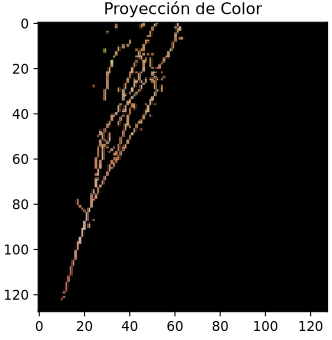
\includegraphics[scale=0.85]{proyeccion_color.pdf}
  \caption{Evento procesado codificando la tercera dimensión en el color de la imagen. Las imágenes han sido procesadas con una resolución de 1000 px y tamaño $128\times128$ px.}
  \label{fig:proy_color}
\end{figure}

\subsection*{Representación para Transformers}

En este trabajo nos vamos a centrar sobre todo en el tratamiento de imágenes y la clasificación se ha realizado utilizando imágenes. Sin embargo, también vamos a plantear una representación distinta, cuya aplicación dejamos como trabajo futuro. Las cascadas tienen un marcado carácter temporal, ya que tenemos un punto inicial donde se origina y, a partir de este punto, esta se va desarrollando. Además, sabemos que al principio es donde se tiene la mayor parte de la información que nos permite hacer la discriminación. Los transformers son una arquitectura que han mostrado muy buenos resultados con textos, que son una estructura de datos donde el orden de las palabras es fundamental.

Estas redes se basan en hacer uso de mecanismos de atención y en codificar la posición de las palabras. Estos modelos se han convertido en el estado del arte del procesamiento de lenguaje natural y nuestra propuesta consiste en utilizar los datos tabulares directamente. Para ello codificamos las instancias temporalmente. En la Fig. \ref{fig:rep_transformer} mostramos gráficamente como proponemos tratar los datos. Si hacemos una analogía con un texto, la idea es que cada evento sea una frase que se le pase al transformer y cada \textit{hit} una palabra. La ``frase'' de \textit{hits} la construimos ordenándolos temporalmente. Los \textit{hits} los representamos con vectores de cuatro elementos, las tres coordenadas espaciales y la carga, al igual que las palabras se representan como vectores.  

Una alternativa, a medio camino entre los métodos presentados, es hacer uso de los Visual Transformers (ViT), que hacen uso de los transformers para trabajar con imágenes. Este modelo particiona la imagen en bloques que se usan como entrada para el transformer. Sin embargo, nuestros datos admiten ser tratados directamente por transformers sin necesidad de pasar por la construcción de la imagen. Por lo tanto, esta forma de funcionar sería mucho más eficiente que el tratamiento con imágenes:

\begin{itemize}
  \item La memoria requerida para almacenar los eventos es muy baja, pues solo necesitamos guardar tantos vectores de cuatro elementos como \textit{hits} tenga el evento.
  \item Con esta representación no se descarta nada de información, puesto que, al contrario que para la generación de imágenes, no necesitamos realizar la proyección ni tomar una ventana del detector.
\end{itemize}


\begin{figure}
  \centering
  \begin{tikzpicture}
    \draw[black, ultra thick] (-2,0) -- (11,0);
    \draw[black, ultra thick] (0,1) -- (0,-6);
    \draw[black, ultra thick] (-0.5,0) -- (-0.5,-6);
    \node[] at (-1.2, 0.3) {Evento};
    \node[align=left] at (4.1, 0.5) {tantas columnas como $hits$ tenga el evento\\ y ordenados temporalmente};    
    \filldraw[color=blue!60, fill=blue!5, ultra thick] (0,0) rectangle (11,-2);
    \node[] at (-0.2, -0.25) {x};
    \node[] at (-0.2, -0.75) {y};
    \node[] at (-0.2, -1.25) {z};
    \node[] at (-0.2, -1.75) {q};
    \node[] at (-1.2, -1) {1};
    \draw[black, ultra thick] (-0,-2) -- (-2,-2);
    \filldraw[color=red!60, fill=red!5, ultra thick] (0,-2) rectangle (5,-4);
    \node[] at (-0.2, -2.25) {x};
    \node[] at (-0.2, -2.75) {y};
    \node[] at (-0.2, -3.25) {z};
    \node[] at (-0.2, -3.75) {q};
    \node[] at (-1.2, -3) {2};
    \draw[black, ultra thick] (-0,-4) -- (-2,-4);
    \filldraw[color=green!60, fill=green!5, ultra thick] (0,-4) rectangle (9,-6);
    \node[] at (-0.2, -4.25) {x};
    \node[] at (-0.2, -4.75) {y};
    \node[] at (-0.2, -5.25) {z};
    \node[] at (-0.2, -5.75) {q};
    \node[] at (-1.2, -5) {3};
    \draw[black, ultra thick] (-0,-6) -- (-2,-6);
    % \draw[blue, ultra thick] (0,0) rectangle (15,0);
    % \filldraw [gray] (0,0) circle (2pt);
    % \node[] at (2.0, -1.5) {$c_x = 8$};

    \node[] at (0.3, -0.25) {x$_1$};
    \node[] at (0.3, -0.75) {y$_1$};
    \node[] at (0.3, -1.25) {z$_1$};
    \node[] at (0.3, -1.75) {q$_1$};

    \node[] at (0.3, -2.25) {x$_1$};
    \node[] at (0.3, -2.75) {y$_1$};
    \node[] at (0.3, -3.25) {z$_1$};
    \node[] at (0.3, -3.75) {q$_1$};

    \node[] at (0.3, -4.25) {x$_1$};
    \node[] at (0.3, -4.75) {y$_1$};
    \node[] at (0.3, -5.25) {z$_1$};
    \node[] at (0.3, -5.75) {q$_1$};
    \draw[black, thick] (0.6,-6) -- (0.6, 0);

    \node[] at (0.9, -0.25) {x$_2$};
    \node[] at (0.9, -0.75) {y$_2$};
    \node[] at (0.9, -1.25) {z$_2$};
    \node[] at (0.9, -1.75) {q$_2$};
    \node[] at (0.9, -2.25) {x$_2$};
    \node[] at (0.9, -2.75) {y$_2$};
    \node[] at (0.9, -3.25) {z$_2$};
    \node[] at (0.9, -3.75) {q$_2$};
    \node[] at (0.9, -4.25) {x$_2$};
    \node[] at (0.9, -4.75) {y$_2$};
    \node[] at (0.9, -5.25) {z$_2$};
    \node[] at (0.9, -5.75) {q$_2$};
    \draw[black, thick] (1.2,-6) -- (1.2, 0);

    \node[] at (1.5, -0.25) {x$_3$};
    \node[] at (1.5, -0.75) {y$_3$};
    \node[] at (1.5, -1.25) {z$_3$};
    \node[] at (1.5, -1.75) {q$_3$};
    \node[] at (1.5, -2.25) {x$_3$};
    \node[] at (1.5, -2.75) {y$_3$};
    \node[] at (1.5, -3.25) {z$_3$};
    \node[] at (1.5, -3.75) {q$_3$};
    \node[] at (1.5, -4.25) {x$_3$};
    \node[] at (1.5, -4.75) {y$_3$};
    \node[] at (1.5, -5.25) {z$_3$};
    \node[] at (1.5, -5.75) {q$_3$};
    \draw[black, thick] (1.8,-6) -- (1.8, 0);

  \end{tikzpicture}
  \caption{Representación gráfica de los datos preparados para el uso de transformers en clasificación de cascadas electromagnéticas. Para cada evento se tienen tantos vectores como $hits$ y cada vector contiene las coordenadas espaciales $(x, y, z)$ y la carga del $hit$ $q$.}
  \label{fig:rep_transformer}
\end{figure}

\section{Arquitecturas}

En esta sección vamos a mostrar las distintas arquitecturas que vamos a emplear para realizar la clasificación de las imágenes. Para esto vamos a usar redes diseñadas desde cero, así como arquitecturas del estado del arte ya entrenadas, donde se modifican tanto los pesos como el clasificador. Las arquitecturas que usaremos serán: EfficientNet, ResNet y GoogleNet. Además, nos hemos basado en LeNet para diseñar una red simple y una más compleja.
 
Independientemente de la arquitectura que se use, es necesario fijar distintos hiperparámetros del algoritmo de aprendizaje, como el ritmo de aprendizaje ($lr$), que pueden ser cruciales de cara a la convergencia y mejora de los resultados.

Como ya hemos dicho, vamos a emplear Pytorch para el diseño y entrenamiento de los modelos. Para esto, primero hay que definir un optimizador, como puede ser SGD o Adam, y, como vamos a considerar un $lr$ dinámico, necesitamos establecer cómo lo vamos a modificar a medida que avance el entrenamiento. Con estos elementos, se implementa el ciclo de aprendizaje del modelo, donde primero se usan todos los \textit{batchs} y se va repitiendo el proceso varias veces (es lo que se conoce como épocas). Cada vez que se completa una época, se validan los resultados con un conjunto de datos no visto por el modelo durante el entrenamiento y, a medida que se avanza en el entrenamiento, se van guardando los pesos aprendidos. Solo se guardan si se mejoran los resultados en validación, es decir, que los pesos del modelo guardado tras el entrenamiento son aquellos con los que mejores resultados se han obtenido en validación.
 
Con la intención de no tener que fijar un número de épocas, lo que hemos hecho ha sido implementar lo que se conoce como parada temprana. Consiste en que si, tras un número consecutivo de épocas, hay mucho sobreajuste o el modelo no mejora en validación, se para el ciclo de aprendizaje y se guardan los pesos con los que mejores resultados se hayan obtenido. De esta forma, no es necesario fijar el número de épocas, pues el entrenamiento se interrumpirá en el momento que ya no se estén mejorando los resultados. % En el Anexo \red{ref} se muestra la en mayor detalle la implementación realizada del ciclo descrito.
 
A continuación, vamos a mostrar como funcionan las distintas arquitecturas que hemos empleado.

\subsection*{LeNet}
\label{sec:lenet}
LeNet es una de las primeras propuestas de redes convolucionales \cite{lenet} que consiste únicamente en aplicar varias veces el bloque convolucional que se mostró en la Sección \ref{sec:dl}. Una vez se extraen las características se realiza la clasificación haciendo uso de un MLP. 

Con estas redes, nuestro objetivo es construir modelos simples para establecer un punto de partida que tratar de mejorar añadiendo complejidad o ajustando los hiperparámetros. Hemos diseñado dos modelos basados en esta arquitectura, uno simple y otro más complejo, donde se aumenta tanto la anchura como la profundidad del modelo simple. Para hacer su diseño, hemos utilizado la representación más simple planteada y probado a modificar el número de filtros por nivel, el número de capas, así como el clasificador.

Las pruebas realizadas serán descritas en la Sección \ref{sec:pruebas_iniciales}, pero mencionar que la construcción de la red nos ha dado muchos problemas, puesto que en muchos casos las redes no superan el 50\% de acierto y pequeños cambios en la estructura de la red hacen que modelo pase de aprender a no aprender. En la Fig. \ref{fig:lenet} se muestran las arquitecturas de los modelos finales que hemos empleado. Tenemos el modelo simple que consiste en dos bloques convolucionales con pocos filtros y un MLP con dos capas ocultas y pocas neuronas. El modelo más complejo es similar al simple, pero hemos modificado el bloque convolucional de manera que se aplican dos capas convolucionales consecutivas sin aplicar la capa de reducción. Además, hemos aumentado la anchura y profundidad de la red, tanto en la extracción de características como en el clasificador.

\begin{figure}[h!]
  \centering
  \includegraphics[scale=0.85, center]{lenet.PNG}
  \caption{Arquitectura basada en LeNet usada para la clasificación de las imágenes dadas. En las capas de convolución se muestran el número de filtros, el tamaño y desplazamiento de los filtros. En las capas de reducción se muestra el tamaño y desplazamiento, y en las capas densas el número de neuronas.}
  \label{fig:lenet}
\end{figure}

\subsection*{EfficientNet}

EfficientNet es una red cuyo objetivo es que sea eficiente y escalable, y que ha mostrado dar muy buenos resultados \cite{enet}. Uno de los problemas fundamentales que se observó tras las primeras CNN es que se tenían problemas para realizar el entrenamiento al aumentar la complejidad de los modelos \cite{resnet}. Con el paso del tiempo, se fueron introduciendo mecanismos para lidiar con este problema y EfficientNet establece una familia con 8 modelos que parten de un modelo base y van aumentando su complejidad.
 
Una red neuronal se puede escalar aumentando la profundidad, la anchura o la resolución (tamaño de las imágenes), EfficientNet lo que hace es introducir un método de escalado que aumenta la complejidad aumentando las tres opciones simultáneamente. Parten de la premisa que las distintas formas de escalar están relacionadas, por ejemplo, si tenemos imágenes más grandes vamos a necesitar más filtros y más capas para conseguir realizar la clasificación \cite{enet}.

% La arquitectura del modelo esta basada en MovilNet v2 \cite{} y ademas hace uso de bloques 

Nosotros vamos a usar estas arquitecturas no solo porque han mostrado dar muy buenos resultados en conjuntos de datos complejos, sino porque, además, nos permite probar una misma arquitectura con distintos niveles de complejidad.

\section*{ResNet}

ResNet es una arquitectura que surge antes que EfficientNet, que introduce también un mecanismo para solucionar problemas a la hora de realizar la optimización cuando se tienen redes muy profundas \cite{resnet}. Está basada en VGG \cite{vgg} que se basa en aplicar sucesivamente bloques convolucionales, creando un modelo muy profundo. ResNet introduce lo que denominan celdas residuales que consisten en agregar la entrada del bloque convolucional a la salida del bloque. A esto le denominan aprendizaje residual y muestran mejoras en la optimización del modelo \cite{resnet}.
 
La arquitectura consiste en aplicar sucesivamente bloques convolucionales y solo se aplica la reducción tras la primera capa convolucional. A esto se le añade el aprendizaje residual. Por otro lado, al igual que para EfficientNet, se tiene una familia de modelos donde varían la profundidad de los modelos. Nosotros usaremos únicamente ResNet 50, donde el 50 hace referencia al número de capas. En la Fig. \ref{fig:resnet} podemos ver la arquitectura de este modelo comparada con la de VGG y la arquitectura de ResNet sin el aprendizaje residual.


\begin{figure}[h!]
  \centering
  \includegraphics[scale=1.0, center]{resnet50.png}
  \caption{Arquitectura de la red ResNet donde se muestra VGG y cómo se modifica para introducir el aprendizaje residual \cite{resnet}.}
  \label{fig:resnet}
\end{figure}

% \section*{GoogleNet}

\section*{Visual Transformer}

Los transformers \cite{transformers} son modelos que se basan únicamente en mecanismos de atención y, actualmente, se han convertido en el estado del arte al trabajar con texto. Los Visual transformers hacen uso de esta arquitectura y la aplican a imágenes. La idea fundamental es que dividen la imagen en bloques y tratan cada bloque como una palabra que el transformers procesa \cite{vit}.

\section{Métricas}

A la hora de realizar un problema de ciencia de datos, es necesario establecer una métrica que nos diga cómo de bueno es nuestro modelo. Como ya se mencionó, en las redes neuronales se define una función pérdida, cuyo gradiente en función de los pesos de la red nos permite modificar estos pesos para mejorar los resultados.
 
Sin embargo, una vez realizado el ajuste, hay distintas métricas que nos permiten evaluar el rendimiento de los modelos, como puede ser el porcentaje de acierto o la curva ROC. Estas métricas nos dan información sobre distintos aspectos, pero en física, para problemas como el que estamos tratando, se suele usar la eficiencia y la pureza.
 
En un problema de clasificación binaria, se tienen dos clases que se suelen denominar como clase positiva y clase negativa. Con el clasificador, se asigna a cada instancia un valor de la clase y pueden darse 4 situaciones:

\begin{itemize}
  \item La instancia sea positiva y el clasificador le asigne la clase positiva. A esto se le denomina positivo real (TP).
  \item La instancia sea negativa y el clasificador le asigne la clase negativa. A esto se le denomina negativo real (TN).
  \item La instancia sea positiva y el clasificador le asigne la clase negativa. A esto se le denomina falso negativo (FN).
  \item La instancia sea negativa y el clasificador le asigne la clase positiva. A esto se le denomina falso positivo (FP).
\end{itemize} 

La eficiencia se define como:
\begin{equation}
  \text{eff} = \frac{\text{TP}}{\text{FN} + \text{TP}},
\end{equation}
es decir, el cociente entre el número de instancias positivas que hemos clasificado bien entre el número de instancias que son realmente positivas.

La pureza se define como:
\begin{equation}
  \text{pureza} = \frac{\text{TP}}{\text{FP} + \text{TP}},
\end{equation}
es decir, el cociente entre las instancias positivas correctamente clasificadas entre las instancias que hemos dicho que son positivas. 

De todos los eventos positivos que se dan en el detector, el porcentaje que hemos sido capaces de clasificar correctamente es la eficiencia. Sin embargo, la pureza nos dice qué porcentaje de los eventos que hemos dicho que son positivos son realmente positivos.
 
En física, dependiendo de la tarea que estemos tratando, nos va a interesar maximizar una u otra. Por ejemplo, en los experimentos donde se pretende descubrir una partícula, se prefiere tener una pureza alta, de manera que si se dice que se tiene dicha partícula realmente, es muy probable que esa afirmación sea cierta. La eficiencia se busca cuando no se quiere perder eventos que realmente sean positivos. Por ejemplo, en un detector Geiger, que determina las partículas radiactivas, nos interesa que tengamos una alta eficiencia para saber cuándo es peligroso un sitio. También es interesante esta última medida cuando la producción de los eventos es cara y descartar eventos tiene un gran coste.  

\section{Hiperparámetros}

Por último, vamos a recoger la mayoría de parámetros que tenemos a la hora realizar el flujo de trabajo completo, denominados hiperparámetros. Vamos a clasificar los hiperparámetros en función de la parte del flujo en la que influyen: El tratamiento de los datos, la arquitectura de la red o el entrenamiento de la red.
 
Antes de entrar en estos bloques, tenemos algunos parámetros generales, como puede ser la semilla aleatoria, que nos permite tener una reproducibilidad de los resultados\footnote{Hay algunas funciones que al usar la GPU no son completamente reproducibles, sin embargo, nuestros modelos no hacen usos de estas funciones.}. Por otro lado, es importante tener en cuenta que el entrenamiento de una red neuronal es algo costoso, tanto en recursos como en tiempo, por lo que no nos podemos permitir hacer búsquedas en rejillas de gran tamaño. Por esto mismo, es fundamental seleccionar aquellos hiperparámetros que más pueden influir en los resultados.

\subsection*{Tratamiento de los datos}

A la hora de hacer la creación de las imágenes, hay un conjunto de parámetros que tenemos que establecer y que, en algunos casos, pueden afectar mucho al resultado obtenido. Los parámetros que tenemos son los siguientes:

\begin{itemize}
  \item \inline{cube_shape_x}: Fija el valor de $c$ en el eje $x$. A partir de este obtenemos los valores en el eje $y$ y $z$.
  \item \inline{win_shape}: Tamaño de la ventana cogida del detector.
  \item \inline{projection}: Tipo de proyección empleada. Como opciones tenemos:  las imágenes tridimensionales, la proyección en cualquiera de los ejes o el tratamiento de color.
  \item \inline{projection_pool} y \inline{cube_pool}: Tratamiento de las situaciones en las tengamos superposición de puntos al realizar el tratamiento. Podemos elegir el máximo o la media.
  \item \inline{log_trans}: Si hacemos o no una transformación logarítmica sobre la carga de los \textit{hits}.
  \item \inline{transform}: Si queremos aplicar una transformación sobre la imagen final. Consiste en hacer uso de la librería \textit{torchvision} que introduce un conjunto de transformaciones como puede ser normalizar lo datos.
\end{itemize}

\subsection*{Arquitectura}

Por otro lado, se tienen distintos parámetros que nos permiten controlar la red que estamos usando para realizar la clasificación. Estos parámetros dependen de si el modelo está  ya entrenado, donde solo podemos controlar el clasificador y el número de capas a reentrenar, o si es un modelo que se construye de cero, donde con los hiperparámetros podemos definir tanto la estructura del extractor como la del clasificador. Los parámetros que tenemos para este apartado son:

\begin{itemize}
  \item \inline{model_name}: Nombre del modelo que vamos a usar.
  \item \inline{conv filters}, \inline{conv_sizes}, \inline{conv_strides}: Tupla que definen el número de capas convolucionales y como son estas capas: número de filtros, tamaño de los filtros y desplazamiento de los filtros.
  \item \inline{pool_sizes} y \inline{pool_strides}: Define el tamaño y el desplazamiento al realizar el \textit{pool}. Son tuplas y tienen que tener el mismo tamaño que los parámetros que definen la convolución.
  \item \inline{clf_neurons}: Tupla con el número de neuronas por cada capa. Cada elemento de la tupla establece una capa.
  \item \inline{clf_no_linear_fun} y \inline{conv_no_linear_fun}: funciones no lineales aplicadas tras las capas densas y las capas de convolución respectivamente.
  \item \inline{bn}: si aplicamos capas de normalizan por \textit{batch}
  % \item n channel: número de canales de la imagen. En caso de tener
  \item \inline{dropout}: Porcentaje de \textit{dropout}. 
\end{itemize}

\subsection*{Entrenamiento de la red}

Por último, tenemos una serie de parámetros que nos permiten regular como se realizar el entrenamiento como puede ser el número de épocas o el tipo de optimizador:

\begin{itemize}
  \item \inline{batch_size}: Tamaño del \textit{batch}.
  \item \inline{n_epochs}: número de épocas.
  \item \inline{optim_name}: tipo de optimizador.
  \item \inline{optim_lr}: ritmo de aprendizaje.
  \item \inline{scheduler_name}: En caso de querer tener un ritmo de aprendizaje que cambie con las épocas cual queremos aplicar.
  \item \inline{scheduler_step_size}: cada cuanto se modifica el ritmo de aprendizaje.
  \item \inline{scheduler_gamma}: cuanto se modifica el ritmo de aprendizaje.
\end{itemize}

Podemos ver que tenemos una gran cantidad de parámetros que podemos modificar y, en muchos casos, pequeñas modificaciones hacen que pasemos de tener modelos que no pasen del 50\% de acierto a modelos que lleguen al 80\%. Por estos motivos, el ajuste de estos hiperparámetros es uno de los aspectos más importantes para obtener un modelo que dé buenos resultados. Para esto, trabajaremos con una metodología concreta que nos permita llegar a ciertas conclusiones y luego ajustar solo los parámetros más relevantes.

\section{Entorno de trabajo}

Por último, vamos a describir algunas peculiaridades del entorno donde hemos realizado los experimentos, que es un aspecto importante al trabajar con redes neuronales, debido a la gran cantidad de recursos que necesitan. Por un lado, vamos a trabajar con redes neuronales y su entrenamiento se beneficia de la gran paralelización de las GPU, sin embargo, el entrenamiento consume muchos recursos, haciendo que en algunos casos un ordenador personal no sea suficiente. La pruebas iniciales se han realizado en un ordenador personal, pero para las pruebas finales hemos recurrido a un cluster de ordenadores que cuenta con 2 procesadores Xeon Silver 4110 (con un total de 32 hebras de procesamiento), 132GB de memoria RAM y 2 GPUs NVidia GeForce RTX 2080 Super. Inicialmente empezamos usando únicamente un portátil\footnote{El portátil cuenta con un procesador Intel i7-7700HQ, 16GB de memoria RAM y una GPU NVidia GTX 1060.}, pero fue necesario hacer uso de un máquina más potente debido al volumen de pruebas, así como por la cantidad de memoria VRAM necesitada. En el Anexo \ref{an:pres} se muestran tanto el la planificación que se ha seguido para resolver este trabajo como el presupuesto necesario para llevarlo a cabo.
 
Otro aspecto fundamental ha sido el control de todos los resultados obtenidos, ya que se han realizado muchas pruebas y ha sido necesario mantener un seguimiento, no solo por conocer los resultados de pruebas antiguas, sino para poder recuperar los modelos que han mostrado buenos resultados y saber los hiperparámetros de estos modelos. Como ya hemos mencionado, vamos hemos utilizado MLFlow para hacer este seguimiento, así como herramienta para hacer el despliegue automático de modelos. Además, nos ha permitido establecer un repositorio central donde poder recoger las métricas y modelos obtenidos en las distintas máquinas usadas\footnote{Para usar el cluster fue necesario hacer una migración de la base de datos que se tenía en local a la nueva base de datos que se creó en el cluster. Esto ha supuesto un reto a nivel técnico, pues fue necesario modificar toda la base de datos porque esta guardaba información de las rutas de los modelos. Por otro lado, también ha habido que configurar MLFlow correctamente para que el repositorio funcionara correctamente.}.

\chapter{Resultados y discusión}
\label{sec:resultados}

En este capítulo, vamos a mostrar los resultados de hacer uso de los distintos modelos que se han presentado junto con las distintas representaciones. En primer lugar vamos a mostrar la metodología seguida, así como una descripción de las pruebas realizadas. A continuación, se mostrarán todas las pruebas junto con sus resultados y comentarios sobre estos. 

% Inicialmente, se muestran las pruebas preliminares realizadas, que nos han permitido entender el problema, su complejidad y establecer un punto de partida. Luego, se han hecho unos estudios que nos permiten determinar, tanto la representación como la resolución de las imágenes. Finalmente, hemos ajustado los parámetros de los modelos que mejores resultados nos han dado y hemos modificado los modelos para tratar de mejorar los resultados.

\section{Metodología de experimentación}

Al final del capítulo anterior se mostró la gran cantidad de hiperparámetros que tenemos, por lo que hacer una búsqueda por todos los parámetros es completamente prohibitiva. Teniendo esto en mente, vamos a definir una metodología de experimentación que nos permita discernir qué representación y resolución de las que se plantean es mejor. Con las mejores representaciones y resoluciones, haremos distintas pruebas sobre los modelos que nos permitan mejorar los resultados.
 
En primer lugar, hemos realizado un conjunto de prueba no estructuradas que nos han permitido entender el problema y comprobar que el tratamiento diseñado es correcto. Asimismo, usamos una de las representaciones para diseñar modelos que funcionen para usarlos en las pruebas futuras.
 
El siguiente punto será determinar cuál de las representaciones que presentamos es mejor. Para esto, probamos las distintas representaciones presentadas para los distintos modelos. En concreto, haremos uso de un modelo simple y uno complejo diseñado por nosotros, distintos modelos EfficientNet, ResNet y GoogleNet. Las pruebas las haremos de manera que se compartan todos los parámetros y que lo único que vamos a modificar son los parámetros del aprendizaje, como el ritmo de aprendizaje, en caso de ser necesario. Una vez hecho este análisis, se pretende obtener una representación que sea mejor que el resto que usaremos para el resto de pruebas.
 
El siguiente paso consiste en escoger una resolución $c_x$, para ello repetiremos el estudio anterior, pero cambiando la resolución. Finalmente, ajustamos los hiperparámetros para intentar superar los resultados obtenidos. Para esto se define una rejilla sobre la que se buscan qué parámetros funcionan mejor. Aplicamos esta búsqueda para los distintos modelos.
 
Una vez hemos obtenido un buen modelo, hemos tratado de mejorar los resultados introduciendo modelos más complejos como pueden ser concatenación de redes (en la Fig. \ref{fig:rep_concat} se muestra el esquema de la arquitectura que mencionamos), o ensembles que nos permitan mejorar los resultados.


\section{Pruebas iniciales}
\label{sec:pruebas_iniciales}

Tras obtener las representaciones y las imágenes, vamos a realizar unos primeros estudios para ver que el procesamiento realizado es correcto y tratar de establecer redes capaces de realizar la clasificación. A continuación, se muestran los experimentos preliminares que han permitido delimitar las pruebas futuras, así como afianzar algunas hipótesis de partida para, posteriormente, hacer su comprobación de manera exhaustiva. Con estas pruebas, queremos estudiar tanto los datos como los modelos para poder establecer una línea de trabajo.
 
Como punto de partida se ha usado la representación más simple y una resolución y tamaño que permitan recoger siempre el comienzo de las cascadas, al ser la zona donde más diferencias se encuentran. Además, hemos tratado de utilizar imágenes pequeñas que nos permitieran construir un modelo con pocos parámetros y establecer un modelo base. Por todo esto, para estas pruebas iniciales, en la mayoría de casos, hemos usado imágenes donde hemos proyectado el eje $y$ y usado una resolución de $c_x = 1000$ px y un de tamaño de ventana de $62 \times 128$ px ($62$ píxeles para el eje $x$ y $128$ para el $z$)
 
En primer lugar, hemos diseñado el modelo LeNet simple que se mostró en la Sección \ref{sec:lenet}. Establecimos un modelo que no fuera especialmente complejo y con pocos filtros, ya que las diferencias fundamentales entre las cascadas son patrones simples como líneas. Además, un modelo simple consume menos recursos y el aprendizaje es más rápido, permitiéndonos hacer un mayor número de pruebas. En definitiva, queremos establecer un modelo base capaz de extraer la máxima información del origen de la cascada.
 
El primer resultado que se obtuvo fue de 67\% de acierto en validación, donde la proyección se hizo sobre el eje $z$. Sin embargo, el máximo se obtuvo con un 88.5\%, tras realizar cambios en la arquitectura, en cómo se creaban las imágenes y en algunos parámetros de interés, así como el eje proyectado escogido, observando que el eje $y$ es el que mejor resultados obtiene. Entrar a comentar todas estas pruebas realizadas no es especialmente interesante al ser más de 100 pruebas, donde muchos de los cambios consisten en realizar ajustes en el tratamiento de las imágenes, tamaño de las imágenes y cambios en la arquitectura de los modelos LeNet y del ciclo de aprendizaje.
 
Sin embargo, sí hay algunas cosas que se han observado que son especialmente interesantes de comentar. Una de las primeras cosas que tratamos de hacer, tras obtener un modelo que mostraba buenos resultados, fue tratar de escalarlo aumentando tanto el número de filtros como el número de capas. No obstante, nos encontramos con que todos los modelos tenían mucha sensibilidad con la semilla de números aleatorios y con la arquitectura de la red, haciendo que en algunos casos se obtuviesen buenos resultados (en torno al $80\%$ de acierto) mientras que en otros casos no se conseguía superar el 50\%, que es lo mismo que usar una moneda para realizar la clasificación.
 
El hecho que los resultados dependan de la semilla es un problema, puesto que nos incapacita para decir que un conjunto de parámetros es malo, ya que podría ser que simplemente estemos en una semilla mala. Para solucionar este problema, probamos a modificar el tamaño del \textit{batch} ($bs$) y cada cuanto se modifica el ritmo de aprendizaje ($lr$). También probamos a modificar el optimizador ($optim.$), aunque vimos que Adam mostraba mejores resultados siempre. El motivo por el que pensábamos que tendría que ser un parámetro relacionado con el aprendizaje, se debe a que el tratamiento de las imágenes no depende de la semilla, por lo que al cambiar la semilla lo que modificamos es: el orden con el que llegan las imágenes al modelo, el conjunto de validación y cómo se realiza el descenso del gradiente. Con distintas pruebas observamos que al aumentar tanto el $bs$ como la frecuencia de cambio del $lr$ se solucionaba este problema.
 
Otra gran cantidad de pruebas fueron hechas con la idea de obtener modelos basados en LeNet, pero más complejos para ver si éramos capaces de mejorar los resultados al obtener patrones más complejos que el modelo simple no fuera capaz de determinar. Sin embargo, nos encontramos con que muchos de los modelos probados no conseguían clasificar el conjunto de datos. Debido a esto, solo hemos conseguido establecer dos modelos de distinta complejidad que consigan clasificar los datos. Las arquitecturas de estos modelos se mostraban en la Fig. \ref{fig:lenet}. A la hora de realizar los estudios posteriores, vamos a usar estos modelos, así como los modelos EfficientNet que tienen distintos niveles de complejidad para ver si modelos más complejos mejoran o empeoran los resultados.
 
\begin{table}[h!]
  \centering
  \begin{tabular}{|c|c|c|c|c|c|}
  \hline
  BN & log & Normalización & dropout & \begin{tabular}[c]{@{}c@{}}Acierto\\ Mejor Val\end{tabular} & \begin{tabular}[c]{@{}c@{}}Acierto\\ Entrenamiento\end{tabular} \\ \hline\hline
  No & No  & No            & 0.0     & 0.885                                                    & 0.892                                                \\ \hline
  No & No  & Sí            & 0.0     & 0.649                                                    & 0.638                                                \\ \hline
  No & Sí  & No            & 0.2     & 0.865                                                    & 0.840                                                \\ \hline
  No & Sí  & Sí            & 0.2     & 0.879                                                    & 0.888                                                \\ \hline
  Sí & No  & No            & 0.35    & 0.884                                                    & 0.875                                                \\ \hline
  Sí & No  & Sí            & 0.35    & 0.638                                                    & 0.87                                                 \\ \hline
  Sí & Sí  & No            & 0.35    & 0.863                                                    & 0.879                                                \\ \hline
  Sí & Sí  & Sí            & 0.35    & 0.866                                                    & 0.865                                                \\ \hline
  \end{tabular}
  \caption{Estudio del efecto de la normalización, capas de normalización por \textit{batch} (BN) y la transformación logarítmica sobre una misma representación. La representación empleada es la proyección en $y$ y el modelo usado es el LeNet simple. El $dropout$ se ha introducido en aquellos casos en los que en los que observaba mucho sobreajuste.}
  \label{tab:transformaciones}
  \end{table}

Antes de entrar a realizar los distintos estudios, se probó a aplicar la transformación logarítmica, así como a introducir capas de normalización por \textit{batch} (BN) \cite{batchnorm}. La introducción de estas modificaciones en la red no mostraron mejoras en los resultados y se observó un aumento en el sobreajuste llegando a obtener cerca de un 100\% de acierto en el conjunto de entrenamiento. Con el uso del \textit{dropout}, se consiguió reducir el sobreajuste llegando a obtener resultados prácticamente idénticos a los obtenidos sin introducir estas modificaciones.

En la Tabla \ref{tab:transformaciones} se muestra el estudio realizado sobre la proyección simple con una resolución de $1000$ px y una ventana de $62\times128$ px. En este estudio, hemos probado todas las combinaciones de introducir o no las capas de BN, la transformación logarítmica y realizar una normalización sobre los píxeles\footnote{Esta normalización se suele aplicar a las imágenes y consiste en aplicar una transformación z-score sobre los distintos canales una vez la imagen está en el rango 0 y 1. Para aplicar esta transformación, se toman como media: $(0.485, 0.456, 0.406)$ y como desviación estándar: $(0.229, 0.224, 0.225)$. En nuestro caso, las imágenes están en este rango, por lo que solo aplicamos la transformación descrita.}. También hemos modificado el \textit{dropout} en aquellos casos donde se tenía sobreajuste, más detalles sobre los hiperparámetros se muestran en el Anexo \ref{an:1}. Los mejores resultados se han obtenido cuando no se ha introducido ninguna de las modificaciones mencionadas. Se han obtenido resultados similares introduciendo la capa de BN. Sin embargo, para obtener estos resultados, es necesario introducir mucho \textit{dropout} debido al sobreajuste. Por lo tanto, se observa que estas técnicas no suponen un mejorar en los resultados, por lo que no vamos a aplicarlas.
% Otro aspecto que es interesante mencionar es que aplicar capas BN no mejora los resultados si solo aplicamos normalización. Esto es relevante porque para los modelos preentrenados se suele aplicar esta normalización, ya que los modelos se han entrenado con imágenes normalizadas de esta forma. Por todo esto, para los próximos experimentos no vamos a hacer uso de estos elementos y solo realizaremos la normalización para los modelos preentrenados.


\section{Selección de una representación}

Las pruebas iniciales nos han servido para entender mejor el conjunto de datos y establecer un punto de partida. Además, la sección anterior nos ha mostrado la cantidad de pruebas que se pueden hacer para mejorar los resultados, poniendo de manifiesto la necesidad de establecer una metodología que nos permita descartar opciones.
 
Lo primero que vamos a hacer es establecer qué representación da mejores resultados de manera general. Para ello, probamos distintos modelos, con distintas complejidades, y determinaremos cuál de ellas es mejor. Para todas las pruebas, hemos usado los mismos parámetros y redes, salvo el ritmo de aprendizaje que se ha modificado solo si el modelo no conseguía superar el 50\%. Las pruebas se han realizado a 10 épocas y con una resolución $c_x = 1000$ px.
 
En la Tabla \ref{tab:estudio_repre} se recogen los resultados para las tres representaciones que hemos presentado, donde para la representación tridimensional no se han realizado pruebas con los modelos preentrenados al no tenerlos accesibles. Por otro lado, para todas las pruebas con modelos preentrenados, hemos usado el mismo clasificador que para el modelo LeNet simple. En el Anexo \ref{an:2} se pueden consultar en detalle los hiperparámetros empleados.

\begin{table}[h!]
  \centering
  \scalebox{0.85}{
  \begin{tabular}{cccccccccc}
  \hline
  \multicolumn{1}{|c|}{}                       & \multicolumn{3}{c|}{Proyección}                                                           & \multicolumn{3}{c|}{Color}                                                                & \multicolumn{3}{c|}{3D}                                                                  \\ \hline
  \multicolumn{1}{|c|}{\% de acierto} & \multicolumn{1}{c|}{train} & \multicolumn{1}{c|}{val.}  & \multicolumn{1}{c|}{mejor val.} & \multicolumn{1}{c|}{train} & \multicolumn{1}{c|}{val.}  & \multicolumn{1}{c|}{mejor val.} & \multicolumn{1}{c|}{train} & \multicolumn{1}{c|}{val.} & \multicolumn{1}{c|}{mejor val.} \\ \hline
  \multicolumn{1}{|c|}{Simple}                   & \multicolumn{1}{c|}{0.892} & \multicolumn{1}{c|}{0.885} & \multicolumn{1}{c|}{0.885}      & \multicolumn{1}{c|}{0.763} & \multicolumn{1}{c|}{0.772} & \multicolumn{1}{c|}{0.772}      & \multicolumn{1}{c|}{0.637}     & \multicolumn{1}{c|}{0.627}    & \multicolumn{1}{c|}{0.627}           \\ \hline
  \multicolumn{1}{|c|}{Complejo}                 & \multicolumn{1}{c|}{0.852} & \multicolumn{1}{c|}{0.866} & \multicolumn{1}{c|}{0.866}      & \multicolumn{1}{c|}{0.856} & \multicolumn{1}{c|}{0.836} & \multicolumn{1}{c|}{0.852}      & \multicolumn{1}{c|}{---}       & \multicolumn{1}{c|}{---}      & \multicolumn{1}{c|}{---}             \\ \hline
  \multicolumn{1}{|c|}{EfficientNet B0}          & \multicolumn{1}{c|}{0.762} & \multicolumn{1}{c|}{0.756} & \multicolumn{1}{c|}{0.768}      & \multicolumn{1}{c|}{0.686} & \multicolumn{1}{c|}{0.641} & \multicolumn{1}{c|}{0.646}      & \multicolumn{1}{c|}{---}       & \multicolumn{1}{c|}{---}      & \multicolumn{1}{c|}{---}             \\ \hline
  \multicolumn{1}{|c|}{EfficientNet B2}          & \multicolumn{1}{c|}{0.688} & \multicolumn{1}{c|}{0.665} & \multicolumn{1}{c|}{0.665}      & \multicolumn{1}{c|}{0.675} & \multicolumn{1}{c|}{0.601} & \multicolumn{1}{c|}{0.610}      & \multicolumn{1}{c|}{---}       & \multicolumn{1}{c|}{---}      & \multicolumn{1}{c|}{---}             \\ \hline
  \multicolumn{1}{|c|}{EfficientNet B5}          & \multicolumn{1}{c|}{0.671} & \multicolumn{1}{c|}{0.613} & \multicolumn{1}{c|}{0.623}      & \multicolumn{1}{c|}{0.659} & \multicolumn{1}{c|}{0.587} & \multicolumn{1}{c|}{0.597}      & \multicolumn{1}{c|}{---}       & \multicolumn{1}{c|}{---}      & \multicolumn{1}{c|}{---}             \\ \hline
  \multicolumn{1}{|c|}{EfficientNet B7}          & \multicolumn{1}{c|}{0.663} & \multicolumn{1}{c|}{0.638} & \multicolumn{1}{c|}{0.643}      & \multicolumn{1}{c|}{0.681} & \multicolumn{1}{c|}{0.601} & \multicolumn{1}{c|}{0.601}      & \multicolumn{1}{c|}{---}       & \multicolumn{1}{c|}{---}      & \multicolumn{1}{c|}{---}             \\ \hline
  \multicolumn{1}{|c|}{ResNet 50}                & \multicolumn{1}{c|}{0.972} & \multicolumn{1}{c|}{0.690} & \multicolumn{1}{c|}{0.731}      & \multicolumn{1}{c|}{0.953} & \multicolumn{1}{c|}{0.607} & \multicolumn{1}{c|}{0.651}      & \multicolumn{1}{c|}{---}       & \multicolumn{1}{c|}{---}      & \multicolumn{1}{c|}{---}             \\ \hline
  \multicolumn{1}{|c|}{GoogleNet}                & \multicolumn{1}{c|}{0.788} & \multicolumn{1}{c|}{0.779} & \multicolumn{1}{c|}{0.779}      & \multicolumn{1}{c|}{0.706} & \multicolumn{1}{c|}{0.659} & \multicolumn{1}{c|}{0.667}      & \multicolumn{1}{c|}{---}       & \multicolumn{1}{c|}{---}      & \multicolumn{1}{c|}{---}             \\ \hline
  \multicolumn{1}{l}{}                           & \multicolumn{1}{l}{}       & \multicolumn{1}{l}{}       & \multicolumn{1}{l}{}            & \multicolumn{1}{l}{}       & \multicolumn{1}{l}{}       & \multicolumn{1}{l}{}            & \multicolumn{1}{l}{}           & ---                           & \multicolumn{1}{l}{}                
  \end{tabular}
  }
  \caption{Porcentajes de acierto para el conjunto de entrenamiento y validación en la última época y el mejor porcentaje de acierto obtenido en validación. Se muestran los resultados obtenidos para distintas representaciones y modelos.}
  \label{tab:estudio_repre}
\end{table}

En la tabla se muestran tanto el mejor porcentaje de acierto en validación (que corresponde al modelo guardado), como los porcentajes en entrenamiento y en validación obtenidos en la última época. Lo más importante que notamos es que, en todos los modelos, los mejores resultados se tienen cuando nos quedamos únicamente con la proyección del eje $y$. Por lo tanto, para el resto de estudios vamos a hacer uso de la proyección simple en este eje. No obstante, es posible que estas diferencias se deban a que no hemos conseguido un modelo capaz de aprender la complejidad añadida al introducir el color. Sin embargo, al no tener ninguna evidencia de esto, no vamos a seguir realizando más pruebas con la proyección de color.  
 
Antes de pasar al resto de pruebas, veamos en detalle los resultados que se recogen en esta tabla. Por un lado, mencionar que el estudio está sesgado con los modelos LeNet, pues estos modelos se han obtenido haciendo uso de la proyección simple, por lo que es posible que se tengan mejores resultados únicamente por esto. Sin embargo, si nos fijamos únicamente en los modelos preentrenados vemos que la proyección simple es mejor en todos los casos.
 
En la representación tridimensional, vemos cómo solo hemos hecho pruebas con el modelo LeNet simple, puel el complejo superaba la memoria de la GPU y no se tiene versión tridimensional de los modelos preentrenados. LeNet si lo podemos usar al haber sido diseñado por nosotros y ser muy simple. Con esta representación, vemos que el resultado obtenidos es considerablemente inferior a los obtenidos con las otras representaciones. Aunque con esta metodología hemos obtenido peores resultados a los obtenidos con las otras representaciones, cuando se hicieron unas pruebas iniciales con este modelo se obtuvo un porcentaje de acierto superior al 70\%. Por lo tanto, es posible que si se probara a modificar parámetros como el $lr$, se podrían mejorar los resultados. Sin embargo, no se han realizado más pruebas debido a la cantidad de recursos que consume, haciendo que el aprendizaje sea muy lento. Por todo esto, consideramos que esta representación no es especialmente interesante de abordar, aunque sí es interesante pensar formas alternativas para abordar el problema. Una opción es utilizar matrices dispersas (\textit{sparse matrix}), que no guardan información de los espacios vacíos. En la literatura se han abordado estos problemas de distintas formas: En \cite{3d_1} se han probado a hacer uso de las arquitecturas del estado del arte y extenderlas a imágenes 3D de manera eficiente, en \cite{3d_sparse} se hace uso de las matrices dispersas en redes convolucionales y en \cite{sparse_neutrino} se aplican estas matrices para la detección de los distintos eventos que tienen lugar dentro del detector que estamos usando nosotros.
 
Aunque, vemos que hay muchos estudios que abordan los problemas que hemos observado con las imágenes tridimensionales, no vamos a entrar en ellos y lo dejamos como un posible área de estudio futuro.
 
Por último, podemos ver como en los modelos EfficientNet, al aumentar la complejidad, los resultados empeoran. Esto puede deberse simplemente a que a mayor complejidad peores resultados, pero también puede ser que, al estar usando en los 4 casos el mismo clasificador, los patrones más complejos no se estén aprendiendo. También puede deberse a que hemos fijado a 10 el número de capas a reentrenar y puede que al tener modelos más complejos sea necesario reentrenar un número mayor de capas. Para los otros dos modelos, observamos que se tienen mejores resultados, aunque para ResNet tenemos mucho sobreajuste. Por todo esto, es interesante probar distintas configuraciones de hiperparámetros con idea de mejorar los resultados o reducir el sobreajuste. 


\section{Selección de la resolución}

Antes de entrar en los ajustes de los modelos, vamos a repetir el estudio anterior, pero variando la resolución en vez de la representación. Cuando se hace referencia a la resolución, estamos haciendo mención al número de píxeles con el que se describe el eje $x$ del detector. Las resoluciones para los otros ejes están relacionadas por la ecuación \ref{eq:resolucion}. Al igual que para el estudio anterior, mostramos los resultados obtenidos en la Tabla \ref{tab:estudio_res} y en el Anexo \ref{an:3} se pueden consultar en detalle los hiperparámetros de las distintas pruebas realizadas.
 
Por un lado, se observa que para los modelos EfficientNet si aumentamos la resolución se tiene una mejora de los resultados, obteniendo los mejores resultados con el modelo B0, que es el más simple. Sin embargo, por el mismo motivo que se comentó en la discusión anterior, no podemos descartar que los modelos más complejos presenten mejores resultados al modificar los hiperparámetros, ya que estamos escalando la complejidad del modelo sin modificar el resto de elementos, por ejemplo el clasificador. Lo que sí parece muy claro es que, si aumentamos la resolución, obtenemos mejores resultados. Esto es muy interesante porque al aumentarla, tenemos una mayor definición en la trayectoria, pero a cambio se reduce la cantidad de cascada que hay en la imagen, puesto que se mantiene el tamaño de la imagen. De esta forma, al aumentar la resolución, nos centramos más en el origen de la cascada, ignorando la parte final.
 
Por otro lado, para LeNet se observa que una vez se supera la resolución de 1000 px, los resultados son similares. Vemos que para resoluciones menores tenemos resultados ligeramente inferiores y que para el modelo simple con la máxima resolución se observa que el modelo no es capaz de superar el 50\%. Esto se  puede deber a los hiperparámetros del modelo, aunque hemos hecho un par de pruebas modificándolos, pero no se han mejorado. Otra opción posible es que hemos aumentado tanto las imágenes, que se pierde mucha cascada como para que el modelo sea capaz de aprender. Sin embargo, viendo que los resultados del modelo simple y complejo son similares para el resto de resoluciones, y que para esta resolución el modelo complejo sí obtiene buenos resultados, es posible que la red no aprenda debido a la primera cuestión mencionada.

Es importante notar que la información que se muestra en los modelos LeNet no es comparable a la información dada a los modelos preentrenados para una misma resolución. Esto se debe a que el tamaño de las imágenes es distinto. En la Fig. \ref{fig:varias_resoluciones} se mostraba el mismo evento para distintas resoluciones, viendo que, a medida que se aumentaba la resolución, se perdía también información. Estas imágenes tenían un tamaño de $128\times128$ px y nosotros estamos usando imágenes $62\times128$ px y $224\times224$ px para los modelos LeNet y preentrenados, respectivamente. Esto quiere decir que, si tenemos una resolución de 1000 px y un tamaño $112\times112$ px, la cantidad de cascada que se recoge es más o menos la misma que se recoge en una imagen con resolución 2000 px pero de tamaño $224\times224$ px\footnote{No es exactamente la misma por el factor 1.25 que hay cuando se obtiene el $c_z$ dado el $c_x$ que es el parámetro de resolución del que hemos hablado en toda la discusión}. Por ende, no debemos de pensar que, a una misma resolución, la información que están recibiendo los modelos es la misma, pues depende también de la ventana.

A modo de resumen, vemos que para los modelos LeNet observamos cómo el resultado satura en una resolución de 1000 px. Observamos que los resultados con resoluciones de 1000 px y de 1500 px son similares, siendo algo mejores para la resolución de 1000 px. No obstante, para el resto de pruebas se ha usado la resolución de 1500 px debido a que, inicialmente, se observan mejores resultados con esta resolución, pero fue tras solucionar un problema en los experimentos, cuando se observó que la resolución de 1000 px era mejor. Este fallo se detectó después de realizar las pruebas de la siguiente sección, por lo que habría que repetir todas las pruebas, que consisten en entrenar 50 modelos. Por este motivo y debido a que las diferencias que se observan entre las resoluciones son muy pequeñas, vamos a quedarnos con la resolución de 1500 px. Además, tener una mayor resolución nos permite definir mejor el origen de la cascada, que es la región que se quería describir con estos modelos LeNet.  

Para los modelos EfficientNet, no se observa que alcancemos un máximo en el rendimiento del modelo al aumentar la resolución, obteniendo los mejores resultados con la última probada, 3000 px. No vamos a probar resoluciones mayores para mantener la máxima información posible, ya que con estos modelos no pretendemos centrarnos únicamente en el origen de la cascada.

\begin{table}[h!]
  \centering
  \begin{tabular}{|c|c|c|c|c|c|c|c|c|}
  \hline
  Resolución (px) & 250   & 500   & 1000  & 1500  & 2000  & 2250   & 2500   & 3000    \\ \hline\hline % & 3500 
  % Simple          & 0.828 & 0.808 & 0.864 & 0.861 & 0.502 & ---    & ---    & ---     \\ \hline       % & ---   
  % Complejo        & 0.730 & 0.815 & 0.871 & 0.876 & 0.874 & ---    & ---    & ---     \\ \hline       % & ---   
  Simple          & 0.834 & 0.855 & 0.885 & 0.881 & 0.502 & ---    & ---    & ---     \\ \hline       % & ---   
  Complejo        & 0.516 & 0.838 & 0.879 & 0.872 & 0.8864 & ---    & ---    & ---     \\ \hline       % & ---   
  EfficientNet B0 & 0.611 & 0.655 & 0.768 & 0.782 & 0.803 & 0.821  & 0.826  & 0.842   \\ \hline       % & 0.837 
  EfficientNet B2 & 0.599 & 0.592 & 0.665 & 0.683 & 0.717 & 0.720  & 0.746  & 0.760   \\ \hline       % & 0.779 
  EfficientNet B5 & 0.582 & 0.579 & 0.623 & 0.666 & 0.693 & 0.719  & 0.716  & 0.738   \\ \hline       % & 0.744 
  \end{tabular}
  \caption{Porcentaje de acierto para distintos modelos y distintas resoluciones (píxeles usados para describir el eje $x$ del detector).}
  \label{tab:estudio_res}
\end{table}

% \begin{figure}[h!]
%   \centering
%   \includegraphics[scale=0.85]{tab_res.pdf}
%   \caption{Porcentajes de acierto en para distintos modelos y distintas resoluciones (píxeles usados para describir el eje $x$ del detector) representado por un mapa de color.}
%   \label{fig:estudio_res}
% \end{figure}

\section{Ajuste de hiperparámetros}

Con todos los resultados observados, surgen algunos aspectos importantes. Vemos que los modelos LeNet obtienen resultados superiores usando imágenes más pequeñas ($62\times 128$) mientras que para los modelos EfficientNet se obtienen siempre peores resultados incluso cuando se usan imágenes de mayor resolución y tamaño. Sin embargo, cabría esperar que los modelos preentrenados obtuviesen mejores resultados que los modelos simples al tener mayor información, resolución y ser modelos más complejos. Por tanto, deberían de ser capaces de extraer patrones más complejos. Además, al haber sido entrenados con muchas imágenes, el entrenamiento debe ser más simple.
 
Por otro lado, los modelos LeNet se diseñaron con la idea de centrarse únicamente en el origen de la cascada al ser el punto donde teóricamente hay más diferencias. Observamos cómo se obtienen muy buenos resultados con una red muy simple. Teniendo todo esto en cuenta, es posible que, para los modelos LeNet, estemos muy cerca del máximo que se puede conseguir teniendo en cuenta que estamos usando una representación desprecia una dimensión completa y que se pierde mucha información al generar las imágenes debido al tamaño y resolución que estamos usando. Por lo mismo, los modelos más complejos deberían al menos igualar a LeNet.
 
Por todo esto, ahora vamos a ajustar los hiperparámetros de los distintos modelos, centrándonos en los modelos preentrenados donde si es esperable una gran mejora. Para los modelos LeNet lo que hemos hecho ha sido ajustar algunos hiperparámetros, pero no esperamos que se consigan mejoras significativas.


% Por un lado vamos a hacer modificaciones sobre los modelos LeNet modificando parámetros como el tamaño de los filtros y su desplazamiento. Además haremos pruebas para distintos ritmos de aprendizaje. Por otro lado haremos pruebas sobre los modelos preentrenados modificando el número de capas a reentrenar así como el el clasificador empleado para clasificar en función de las características aprendidas.

\subsection*{LeNet}

\begin{table}[h!]
  \centering
  \begin{tabular}{|cc||cc|cc|cc|cc|}
  \hline
  \multicolumn{2}{|c||}{\multirow{2}{*}{}}    & \multicolumn{1}{c|}{ks}         & kd        & \multicolumn{1}{c|}{ks}         & kd        & \multicolumn{1}{c|}{ks}         & kd        & \multicolumn{1}{c|}{ks}         & kd        \\ \cline{3-10} 
  \multicolumn{2}{|c||}{}                     & \multicolumn{1}{c|}{3}          & 1         & \multicolumn{1}{c|}{5}          & 1         & \multicolumn{1}{c|}{3}          & 2         & \multicolumn{1}{c|}{5}          & 2         \\ \hline\hline
  \multicolumn{1}{|c|}{lr}       & 10$^{-3}$ & \multicolumn{2}{c|}{\multirow{2}{*}{0.883}} & \multicolumn{2}{c|}{\multirow{2}{*}{0.891}} & \multicolumn{2}{c|}{\multirow{2}{*}{0.771}} & \multicolumn{2}{c|}{\multirow{2}{*}{0.718}} \\ \cline{1-2}
  \multicolumn{1}{|c|}{$\gamma$} & 1.0       & \multicolumn{2}{c|}{}                       & \multicolumn{2}{c|}{}                       & \multicolumn{2}{c|}{}                       & \multicolumn{2}{c|}{}                       \\ \hline
  \multicolumn{1}{|c|}{lr}       & 10$^{-3}$ & \multicolumn{2}{c|}{\multirow{2}{*}{0.884}} & \multicolumn{2}{c|}{\multirow{2}{*}{0.892}} & \multicolumn{2}{c|}{\multirow{2}{*}{0.768}} & \multicolumn{2}{c|}{\multirow{2}{*}{0.727}} \\ \cline{1-2}
  \multicolumn{1}{|c|}{$\gamma$} & 0.8       & \multicolumn{2}{c|}{}                       & \multicolumn{2}{c|}{}                       & \multicolumn{2}{c|}{}                       & \multicolumn{2}{c|}{}                       \\ \hline
  \multicolumn{1}{|c|}{lr}       & 10$^{-3}$ & \multicolumn{2}{c|}{\multirow{2}{*}{0.881}} & \multicolumn{2}{c|}{\multirow{2}{*}{0.887}} & \multicolumn{2}{c|}{\multirow{2}{*}{0.763}} & \multicolumn{2}{c|}{\multirow{2}{*}{0.728}} \\ \cline{1-2}
  \multicolumn{1}{|c|}{$\gamma$} & 0.7       & \multicolumn{2}{c|}{}                       & \multicolumn{2}{c|}{}                       & \multicolumn{2}{c|}{}                       & \multicolumn{2}{c|}{}                       \\ \hline
  \multicolumn{1}{|c|}{lr}       & 10$^{-3}$ & \multicolumn{2}{c|}{\multirow{2}{*}{0.875}} & \multicolumn{2}{c|}{\multirow{2}{*}{0.886}} & \multicolumn{2}{c|}{\multirow{2}{*}{0.762}} & \multicolumn{2}{c|}{\multirow{2}{*}{0.718}} \\ \cline{1-2}
  \multicolumn{1}{|c|}{$\gamma$} & 0.5       & \multicolumn{2}{c|}{}                       & \multicolumn{2}{c|}{}                       & \multicolumn{2}{c|}{}                       & \multicolumn{2}{c|}{}                       \\ \hline
  \multicolumn{1}{|c|}{lr}       & 10$^{-4}$ & \multicolumn{2}{c|}{\multirow{2}{*}{0.818}} & \multicolumn{2}{c|}{\multirow{2}{*}{0.862}} & \multicolumn{2}{c|}{\multirow{2}{*}{0.627}} & \multicolumn{2}{c|}{\multirow{2}{*}{0.593}} \\ \cline{1-2}
  \multicolumn{1}{|c|}{$\gamma$} & 1.0       & \multicolumn{2}{c|}{}                       & \multicolumn{2}{c|}{}                       & \multicolumn{2}{c|}{}                       & \multicolumn{2}{c|}{}                       \\ \hline
  \multicolumn{1}{|c|}{lr}       & 10$^{-4}$ & \multicolumn{2}{c|}{\multirow{2}{*}{0.758}} & \multicolumn{2}{c|}{\multirow{2}{*}{0.836}} & \multicolumn{2}{c|}{\multirow{2}{*}{0.597}} & \multicolumn{2}{c|}{\multirow{2}{*}{0.573}} \\ \cline{1-2}
  \multicolumn{1}{|c|}{$\gamma$} & 0.8       & \multicolumn{2}{c|}{}                       & \multicolumn{2}{c|}{}                       & \multicolumn{2}{c|}{}                       & \multicolumn{2}{c|}{}                       \\ \hline
  \multicolumn{1}{|c|}{lr}       & 10$^{-4}$ & \multicolumn{2}{c|}{\multirow{2}{*}{0.713}} & \multicolumn{2}{c|}{\multirow{2}{*}{0.803}} & \multicolumn{2}{c|}{\multirow{2}{*}{0.612}} & \multicolumn{2}{c|}{\multirow{2}{*}{0.584}} \\ \cline{1-2}
  \multicolumn{1}{|c|}{$\gamma$} & 0.7       & \multicolumn{2}{c|}{}                       & \multicolumn{2}{c|}{}                       & \multicolumn{2}{c|}{}                       & \multicolumn{2}{c|}{}                       \\ \hline
  \multicolumn{1}{|c|}{lr}       & 10$^{-4}$ & \multicolumn{2}{c|}{\multirow{2}{*}{0.657}} & \multicolumn{2}{c|}{\multirow{2}{*}{0.764}} & \multicolumn{2}{c|}{\multirow{2}{*}{0.609}} & \multicolumn{2}{c|}{\multirow{2}{*}{0.578}} \\ \cline{1-2}
  \multicolumn{1}{|c|}{$\gamma$} & 0.5       & \multicolumn{2}{c|}{}                       & \multicolumn{2}{c|}{}                       & \multicolumn{2}{c|}{}                       & \multicolumn{2}{c|}{}                       \\ \hline
  \end{tabular}
  \caption{Porcentajes de aciertos en validación de los modelos obtenidos en la búsqueda de rejilla realizada sobre el modelo LeNet simple. Se han modificado el ritmo de aprendizaje ($lr$), la cantidad que se modifica el $lr$ ($\gamma$), el tamaño de los filtros ($ks$) y su desplazamiento ($ks$).}
  \label{tab:resultados_kernel_simple}
\end{table}

\begin{table}[h!]
  \centering
  \begin{tabular}{|cc||cc|cc|cc|cc|}
  \hline
  \multicolumn{2}{|c||}{\multirow{2}{*}{}} & \multicolumn{1}{c|}{ks} & kd & \multicolumn{1}{c|}{ks} & kd & \multicolumn{1}{c|}{ks} & kd & \multicolumn{1}{c|}{ks} & kd \\ \cline{3-10} 
  \multicolumn{2}{|c||}{}                  & \multicolumn{1}{c|}{3}  & 1  & \multicolumn{1}{c|}{5}  & 1  & \multicolumn{1}{c|}{3}  & 2  & \multicolumn{1}{c|}{5}  & 2  \\ \hline\hline
  \multicolumn{1}{|c|}{$\gamma$}   & 1.0  & \multicolumn{2}{c|}{0.875}   & \multicolumn{2}{c|}{0.857}   & \multicolumn{2}{c|}{0.516}   & \multicolumn{2}{c|}{0.858}   \\ \hline
  \multicolumn{1}{|c|}{$\gamma$}   & 0.8  & \multicolumn{2}{c|}{0.879}   & \multicolumn{2}{c|}{0.857}   & \multicolumn{2}{c|}{0.516}   & \multicolumn{2}{c|}{0.526}   \\ \hline
  \multicolumn{1}{|c|}{$\gamma$}   & 0.5  & \multicolumn{2}{c|}{0.870}   & \multicolumn{2}{c|}{0.767}   & \multicolumn{2}{c|}{0.516}   & \multicolumn{2}{c|}{0.484}   \\ \hline
  \end{tabular}
  \caption{Porcentajes de aciertos en validación de los modelos obtenidos en la búsqueda de rejilla realizada sobre el modelo LeNet complejo. Se han modificado la cantidad que se modifica el $lr$ ($\gamma$), el tamaño de los filtros ($ks$) y su desplazamiento ($ks$).}
  \label{tab:resultados_kernel_complejo}
\end{table}

Como ya hemos puesto de manifiesto en varias ocasiones, tenemos una gran cantidad de parámetros y no nos podemos permitir hacer una búsqueda sobre todos ellos. Por todo esto, vamos a probar a modificar 4 parámetros: el ritmo de aprendizaje ($lr$), lo que se modifica el ritmo de aprendizaje cada época ($\gamma$), el tamaño de los filtros ($ks$) y el desplazamiento ($kd$). Las pruebas las vamos a realizar para ambos modelos y en las Tablas \ref{tab:resultados_kernel_simple} y \ref{tab:resultados_kernel_complejo}, se recogen los resultados. En el Anexo \ref{an:4} se muestran los hiperparámetros en detalle.
 
En la rejilla definida con estos parámetros, solo hemos probado un par de valores para cada parámetro. Aun así, el número de pruebas realizadas al final, ha sido en torno a 50, ya que se han realizado algunas más y descartado otras. En concreto, hemos hecho 32 pruebas para el modelo simple y 15 para el complejo y la rejilla consiste en:

\begin{itemize}
  \item \inline{optim_lr} $\in \left[0.0001, 0.001\right]$.
  \item \inline{scheduler_gamma} $\in \left[0.5, 0.7, 0.8, 1\right]$.
  \item \inline{kernel_stride} $\in \left[1, 2\right]$.
  \item \inline{kernel_size} $\in \left[3, 5\right]$.
\end{itemize}

Para estudiar los resultados hemos usado MLFlow que, además, nos permite comparar experimentos y hacer gráficas mostrando los distintos hiperparámetros y los resultados de esos experimentos. En la Fig. \ref{fig:estudio_kernel} se muestra un ejemplo de la gráfica obtenida y, además, se pueden seleccionar rangos de parámetros para visualizar correctamente modelos concretos. Las conclusiones que podemos llegar de los resultados del modelo simple son:
 
\begin{itemize}
  \item Siempre se observa que los resultados son peores cuando se usa un desplazamiento de los filtros de 2 px frente a usar un $kd = 1$ px.
  \item De igual manera, se observa con el $lr$, donde el $lr = 0.0001$ siempre da peores resultados frente a usar $lr = 0.001$. El resto de conclusiones las vamos a limitar estos casos.
  \item También vemos que, en general, a medida que disminuimos el $\gamma$ vemos que los resultados empeoran pero el máximo se encuentra en 0.8 siendo ligeramente peor cuando el gamma es 1.0.
  \item Siempre se observan mejores resultados con los filtros 5 px de tamaño.
  \item El mejor resultado se tiene con un 0.892 para $lr = 0.001$, $\gamma = 0.8$, $ks = 5$ px y $kd = 1$ px.
\end{itemize}

\begin{figure}[h!]
  \centering
  \includegraphics[scale=0.65, center]{studio_kernel_simple.PNG}
  \caption{Gráfica obtenida de MLFlow con los resultados de la búsqueda de rejilla aplicada sobre el modelo simple con una resolución de 1500 px.}
  \label{fig:estudio_kernel}
\end{figure}
 
Para el modelo complejo, hemos usado un valor de $\gamma$ menos y vimos que, cuando se tenía $lr = 0.001$, el modelo no aprendía, por lo que no se realizaron todas las pruebas con este $lr$. Además, hemos tenido que modificar las imágenes introduciendo lo que se denomina \textit{padding} para que, al aplicar los filtros, se puedan utilizar los píxeles en los bordes y no se reduzca mucho la imagen. El método de \textit{padding} empleado consiste en ampliar la imagen añadiendo píxeles negros fuera de la imagen. Con estas pruebas se observó que:
\begin{itemize}
 
  \item Siempre se obtienen mejores resultados cuando el desplazamiento es de 1 px.
  \item Con respecto al $\gamma$ vemos que los mejores resultados se tienen con $\gamma = 0.8$ y parece que lo mejor es cuando es 0.8 ó 1.0.
  \item A diferencia que lo que se observaba con el modelo simple, se obtiene mejores resultados con el $ks = 3$ px.
  \item El mejor resultado se tiene con un 0.879 para $lr = 0.0001$, gamma = 0.7, $ks = 3$ px y $kd = 1$ px.
\end{itemize}
 
En resumen, vemos cómo el uso de filtros de mayor tamaño mejora ligeramente los resultados obtenidos con el modelo simple. Notar que la mejora obtenida es de un 1\% que es considerablemente bajo, teniendo en cuenta que hemos hecho más de 50 pruebas para llegar a este modelo.
 
Por otro lado, aunque es posible que se mejoren aún más los resultados si buscamos en otros parámetros, sería necesario realizar muchas más pruebas con el gran coste de energético y de tiempo que eso conlleva. Además, previamente a este trabajo, el grupo de investigación con el que se está realizado este trabajo, ha abordado la resolución del mismo problema que hemos presentado nosotros, usando otros algoritmos de ML. Para ello se han utilizando los datos tabulares codificados de manera que se mantiene toda la información de la cascada. Tras el ajuste que acabamos de presentar, nuestros resultados ya son similares a los obtenidos en este estudio utilizando modelos como Random Forest \cite{auu}. Esto nos muestra que nuestro modelo más simple ya obtiene muy buenos resultados y cómo el origen de las cascadas ya nos permite obtener resultados satifactorios desde el punto de vista físico.

\subsection*{Modelos preentrenados}

Una vez hemos ajustado los modelos LeNet, veamos los modelos preentrenados. Lo primero que vamos a hacer es tratar de establecer un valor de $\gamma$ y \textit{lr}. Como no podemos hacer esto para todos los modelos, hacemos primero una prueba inicial con un clasificador complejo, un extractor de complejidad intermedia, como EfficientNet B2, y usaremos un \textit{dropout} de 0.2. El clasificador utilizado tiene una única capa oculta con 256 neuronas. Además, se han descongelado 50 capas y se han probado 3 valores de $\gamma$: $\left[1.0, 0.8, 0.5\right]$ y 3 valores de \textit{lr}: $\left[0.0001, 0.001, 0.01\right]$. Los mejores resultados se han obtenido con el $\gamma$ más bajo y el \textit{lr} más alto. Estos resultados se muestran en la Fig. \ref{fig:studio_optim} y se pueden consultar detenidamente en el Anexo \ref{an:6}.
 
\begin{figure}[h!]
  \centering
  \includegraphics[scale=0.65, center]{studio_optim_pre.png}
  \caption{Gráfica obtenida de MLFlow con los resultados de la búsqueda inicial del $lr$ y de $\gamma$.}
  \label{fig:studio_optim}
\end{figure}

Con estos valores de $\gamma$ y \textit{lr}, definimos una rejilla donde se modifica el clasificador y el número de capas descongeladas del extractor de características. Los clasificadores tienen una única capa oculta con 256 y 128 neuronas ($n_n$) y el número de capas a descongelar ($n_u$) probados son $\left[5, 50, 100, 300, 1000 \right]$. Hemos fijado el \textit{dropout} ($dr$) a 0.3, ya que, en general, hemos visto que se tiene sobreajuste con estos modelos. Por otro lado, en algunas ocasiones las pruebas de $n_u = 1000$ no se han realizado por no tener memoria suficiente, pues los modelos que estamos usando llegan a tener muchas capas y pesos. Hemos introducido $n_u=1000$ como caso en el que se descongelan todas las capas.  
 
Estas pruebas se hicieron en primer lugar usando únicamente los modelos EfficientNet B0, B2 y B5 para ver si de esta forma podríamos reducir el número de pruebas al observar algún patrón. En la Tabla \ref{tab:res_ajuste_pre} se recogen los resultados en validación de la búsqueda de rejilla sobre estos modelos, así como las pruebas realizadas utilizando ResNet y GoogleNet. En el Anexo \ref{an:7}, se pueden consultar los detalles de los hiperparámetros.

\begin{table}[h!]
  \centering
  \begin{tabular}{|c||cc|cc|cc|c|c|}
  \hline
  \multirow{2}{*}{} & \multicolumn{2}{c|}{B0}            & \multicolumn{2}{c|}{B2}            & \multicolumn{2}{c|}{B5}             & ResNet & GoogleNet \\ \cline{2-9} 
                    & \multicolumn{1}{c|}{256}   & 128   & \multicolumn{1}{c|}{256}   & 128   & \multicolumn{1}{c|}{256}    & 128   & 256    & 256       \\ \hline\hline
  5                 & \multicolumn{1}{c|}{0.737} & 0.838 & \multicolumn{1}{c|}{0.749} & 0.756 & \multicolumn{1}{c|}{0.729}  & 0.728 & 0.779  & 0.837     \\ \hline
  50                & \multicolumn{1}{c|}{0.884} & 0.878 & \multicolumn{1}{c|}{0.826} & 0.819 & \multicolumn{1}{c|}{0.808}  & 0.811 & 0.878  & 0.869     \\ \hline
  100               & \multicolumn{1}{c|}{0.889} & 0.516 & \multicolumn{1}{c|}{0.872} & 0.870 & \multicolumn{1}{c|}{0.516}  & 0.516 & 0.516  & 0.880     \\ \hline
  300               & \multicolumn{1}{c|}{0.898} & 0.839 & \multicolumn{1}{c|}{\textbf{0.913}} & 0.904 & \multicolumn{1}{c|}{0.859*} & 0.859 & 0.569  & 0.516     \\ \hline
  1000              & \multicolumn{1}{c|}{0.898} & 0.839 & \multicolumn{1}{c|}{0.854} & 0.516 & \multicolumn{1}{c|}{---}    & ---   & 0.569  & 0.516     \\ \hline
  \end{tabular}
  \caption{Porcentajes de acierto en validación de los modelos obtenido en una búsqueda de rejilla donde se ha modificado el número de capas a reentrenar y el clasificador. Se muestran los resultados para distintos modelos preentrenados. La primera columna hace referencia al número de capas descongeladas $n_u$, la primera fila al modelo y la segunda al número de neuronas del clasificador $n_n$. El asterisco significa que se ha entrenado con 15 épocas.}
  \label{tab:res_ajuste_pre}
\end{table}

En primer lugar, se observa es que los resultados son muy superiores a los obtenidos sin realizar la modificación de los parámetros, mostrando cómo de importante puede ser el ajuste. Por otro lado, el mejor resultado se obtiene con el modelo B2 con $n_u = 300$ y con $n_n = 256$ obteniendo un 91.3\% de acierto en validación que es una mejora considerable a los resultados obtenidos con los modelos LeNet.
 
Podemos sacar algunas conclusiones de estos resultados. Vemos que para los modelos EfficientNet, en general, se tienen mejores resultados cuando se usa $n_n = 256$, por lo que para los otros modelos se decidió usar solo este valor. Con respecto a $n_u$, observamos que los resultados mejoran al aumentar este parámetro hasta que se alcanza un máximo, a partir del cual los resultados empeoran. Una posible explicación es que, al ir aumentando el número de pesos que se pueden ajustar, se llegue a un punto donde haya tantos pesos por ajustar que la red tenga problemas para hacerlo, dando lugar a peores resultados.
 
Por otro lado, vemos que los resultados obtenidos con los modelos B5, ResNet y GoogleNet son ligeramente inferiores a los obtenidos con otros modelos, pero esto puede deberse únicamente al espacio de búsqueda establecido. Sobre estos modelos hemos hecho algunas pruebas adicionales para ver si se conseguían mejorar un poco más los resultados, especialmente para aquellos en los que se han obtenido malos resultados.

\begin{itemize}
  \item ResNet 50: Hemos probado a usar $dr = 0.4$ para $n_u = 50, 100$ obteniendo 0.883, 0.891 respectivamente. Obteniendo una mejora considerable y similar a los mejores resultados obtenidos con el resto de modelos.
  \item GoogleNet: También hemos probado a usar el $dr = 0.4$ para $n_u = 100, 300$ obteniendo 0.892 y 0.516. Donde vemos que para $n_u = 100$ hemos mejorado el porcentaje de acierto llegando también a igualar al resto de modelos. También hemos probado a usar $n_n = 128$ obteniendo 0.808.
  \item B5: Hemos usado $n_n = 512$ para el caso que peores resultados tenía obteniendo 0.819.
  \item B0: Hemos probado a introducir $dr = 0.4$ para los mejores resultados pero se han empeorado los resultados.
\end{itemize}
 
A modo de conclusión de las pruebas que hemos realizado, vemos que en la mayoría de pruebas se supera el 0.89, de hecho, solo el B5 no lo ha conseguido. Por otro lado, vemos que el B0 y B2 son los que mejores resultados han dado, sobre todo el modelo B2 que supera en un 2-3\% al resto de modelos. En general, vemos que las diferencias entre los modelos no es muy alta, siendo posible que las diferencias se deban a los hiperparámetros, es decir, parece que todos los modelos son más o menos similares. Esto es coherente con las imágenes que estamos usando, pues, aunque a simple vista es muy difícil determinar el origen de la cascada, los patrones que las diferencian son en su mayoría simples.

Como ya hemos repetido varias veces, no podemos afirmar que este sea el mejor modelo, pues no hemos hecho suficientes pruebas y puede que ajustar más algunos parámetros hagan que los otros modelos lo igualen o incluso lo superen. Sin embargo, el número de pruebas necesario para esto es muy alto y, con las pruebas ya realizadas, vemos cómo hemos conseguido unos resultados muy buenos. En este punto, es más interesante modificar las arquitecturas con la idea de tratar de recoger la información que estamos perdiendo al construir las imágenes que seguir con la búsqueda de hiperparámetros. Para estas modificaciones haremos uso de EfficientNet B2 al ser el que mejores resultados nos ha dado. En caso de tener problemas por la complejidad del modelo, usaremos alguno más simple.


\section{Breve estudio del modelo B2}
 
Antes de hacer las modificaciones sobre la arquitectura, vamos a tratar de elaborar un breve estudio del modelo obtenido. Recordemos que estos modelos son ``cajas negras'' cuya interpretación es muy compleja. En esta sección, vamos a ver algunas métricas que nos digan cómo de bueno es el modelo y veremos las imágenes en las que el modelo se está equivocando.
%  y probaremos a usar una técnica que nos permita visualizar las regiones de la imagen que más influyen en la decisión.
Además, obtendremos la eficiencia y pureza del modelo en función de la energía y veremos cómo se modifican los resultados si quitamos \textit{hits} de la imagen.
 
En la Tabla \ref{tab:res_modelo_def}, se muestran distintas métricas para evaluar el modelo para los distintos conjuntos de datos, donde se recogen el porcentaje de acierto, el F1, el AUC, la eficiencia y la pureza. Por un lado, vemos cómo prácticamente no tenemos sobreajuste, hay una diferencia en torno a un 1\% entre los resultados de entrenamiento y de prueba. Por otro lado, tenemos una pureza muy superior a la eficiencia, es decir, tenemos muchos eventos que clasificamos como fotones, pero son electrones (muchos falsos positivos que reducen la eficiencia). Sin embargo, tenemos muy pocos eventos que clasificamos como electrones si son fotones (pocos falsos negativos por los que aumentamos la pureza). Esto último lo podemos ver en la matriz de confusión del conjunto de prueba que se muestra en la Fig. \ref{fig:con_mat}. Con todo esto podemos ver cómo hemos obtenido un modelo que obtiene muy buenos resultados, sobre todo en la pureza, que es especialmente interesante al estar trabajando en un problema de descubrimiento de una nueva partícula.

\begin{figure}[h!]
  \centering
  \includegraphics[scale=0.65, center]{conmat.pdf}
  \caption{Matriz de confusión obtenida usando el mejor modelo EfficientNet B2 obtenido sobre el conjunto de prueba.}
  \label{fig:con_mat}
\end{figure}

\begin{table}[h!]
  \centering
  \begin{tabular}{|c|c|c|c|}
  \hline
                                                                  & Entrenamiento & Validación & Prueba \\ \hline
  \begin{tabular}[c]{@{}c@{}}Porcentaje\\ de acierto\end{tabular} & 91.8          & 91.3       & 90.4   \\ \hline
  F1                                                              & 0.921         & 0.920      & 0.909  \\ \hline
  AUC                                                             & 0.979         & 0.968      & 0.967  \\ \hline
  Eficiencia                                                      & 0.865         & 0.854      & 0.840  \\ \hline
  Pureza                                                          & 0.967         & 0.961      & 0.962  \\ \hline
  \end{tabular}
  \caption{Resultados para distintas métricas del mejor modelo obtenido usando la proyección del eje $y$ y con el model EfficientNet B2.}
  \label{tab:res_modelo_def}
\end{table}

Por otro lado, en la Fig. \ref{fig:eff_pur} se muestra cómo evolucionan la eficiencia y la pureza en función de la energía, así como con el producto de estas dos métricas. Por un lado, podemos ver cómo la pureza se mantiene más o menos constante con la energía, mientras que la eficiencia es ligeramente peor a bajas energías. Podemos ver cómo, aunque es más o menos constante con la energía, si se observa que el rendimiento es ligeramente inferior a bajas energías, sobre todo en la eficiencia. No obstante, tenemos que tener en cuenta que, en estos casos, los eventos están dados por 5-10 $hits$ y que, con esta poca información, el modelo es capaz de determinar bastante bien el tipo de cascada observada.


\begin{figure}[h!]
  \centering
  \includegraphics[scale=0.55, center]{test.pdf}
  \caption{Eficiencia y pureza del mejor modelo EfficientNet B2 obtenidas sobre el conjunto de prueba al variar la energía.}
  \label{fig:eff_pur}
\end{figure}

A continuación, vamos a ver cómo se comporta el modelo si lo entorpecemos quitando $hits$ de los eventos con la idea de interpretar, dentro de lo posible, el modelo obtenido. Para esto, hemos quitado de los $hits$ de tres formas distintas: aleatoriamente, por energía y temporalmente.
 
En la Fig. \ref{fig:pur_alea} se muestra cómo influye en el modelo que se pierdan un porcentaje aleatorio de los \textit{hits}. En esta gráfica, se observa cómo tenemos una disminución progresiva de los resultados al ir reduciendo la cantidad de píxeles que el modelo recibe hasta que llega un punto, a partir del cual el modelo predice aleatoriamente que tipo de partícula origina el evento. En la Fig. \ref{fig:pur_ene} se muestra una gráfica equivalente, pero ahora estamos quitando gradualmente los \textit{hits} más energéticos. Vemos cómo si quitamos solo los más energéticos la diferencia es mínima, no obstante, a medida que aumenta la cantidad de \textit{hits} que quitamos, vemos cómo la pureza comienza a disminuir hasta que llega a tener una pureza inferior al 50\%. Esto que observamos es interesante, pues parece que los \textit{hits} menos energéticos son más importantes para clasificar fotones. Por esto, cuando el modelo recibe únicamente estos, se observa un aumento de los falsos negativos, es decir, muchos eventos que son electrones se predicen como fotones porque le estamos dando los rasgos que usa el modelo para determinar los fotones. También lo podemos ver al contrario, la red usa los más energéticos para identificar los electrones, pero al no verlos en la imagen, esta asume que es un fotón.

\begin{figure}[h!]
  \centering
  \includegraphics[scale=0.59, center]{pureza_alea.pdf}
  \caption{Evolución de la pureza al reducir de forma aleatoria en número de \textit{hits} que recibe el modelo para realizar la clasificación.}
  \label{fig:pur_alea}
\end{figure}

\begin{figure}[h!]
  \centering
  \includegraphics[scale=0.59, center]{pureza_ene.pdf}
  \caption{Evolución de la pureza al reducir de forma progresiva los \textit{hits} que recibe el modelo para realizar la clasificación de más energéticos a menos.}
  \label{fig:pur_ene}
\end{figure}

\begin{figure}[h!]
  \centering
  \includegraphics[scale=0.55, center]{pur_temp.pdf}
  \caption{Evolución de la pureza al reducir de forma progresiva los \textit{hits} que recibe el modelo para realizar la clasificación. Primero se eliminan los \textit{hits} producidos más tardes hasta llegar a los más nuevos.}
  \label{fig:pur_tem}
\end{figure}

Por último, en la Fig. \ref{fig:pur_tem} se muestra cómo influye en el rendimiento del modelo que quitemos los \textit{hits} ordenados temporalmente, es decir, para cada imagen quitamos una fracción de los \textit{hits} empezando por los que se produjeron más tarde\footnote{Concretamente, lo que hacemos es crear una variable que tenga los \textit{hits} y el tiempo, obtenemos los cuantiles y nos quedamos solo con la fracción más temprana. Es decir, obtenemos un valor de tiempo que hace que mantengamos un porcentaje concreto de \textit{hits}.}. Vemos cómo el comportamiento es muy distinto al observado en las gráficas anteriores. Si nos fijamos en el eje $x$ de la Fig. \ref{fig:pur_tem}, no se observa una caída en el rendimiento hasta que se reduce la fracción por debajo del 0.05, es decir, nos quedamos solo con unos pocos \textit{hits} del principio de la cascada. Estos resultados nos están mostrando cómo el modelo está realizando la clasificación utilizando únicamente los primeros \textit{hits}, siendo el resto inenecesarios para la discriminación.

Cómo ya se ha mencionado anteriormente, el grupo de investigación con el que se está realizando este trabajo, hizo uso de métodos de ML no basados en DL para resolver el mismo problema que se trata aquí. Los resultados que se obtuvieron con estos métodos mostraban un comportamiento similar al que se observa con el modelo aquí presentado: usar la cascada completa no mejora los resultados si se usa únicamente el origen. Este resultado es coherente con la física del problema, pues sabemos que la diferencia entre las cascadas se encuentra en su mayoría en el origen. No obstante, hay información en otras regiones pero nuestro modelo no está siendo capaz de aprenderla dejando un posible margen de mejora. 
 
Finalmente, podemos ver en que imágenes el modelo se ha equivocado y en cuales el modelo ha clasificado correctamente. Para esto hemos hecho uso de Jupyter Notebook, donde se muestran eventos aleatorios ordenados por clase. Además, lo hemos hecho de manera que se muestren por separado imágenes donde el modelo acierta y donde se equivoca para cada clase. En la Fig. \ref{fig:muchas} mostramos la gráfica generada por el código y nos permite visualizar las imágenes con la idea visualizar si hay algún problema o ver si podemos observar algún patrón en las imágenes que el modelo confunde.

\begin{figure}[h!]
  \centering
  \includegraphics[scale=0.45, center]{muchas.pdf}
  \caption{Distintos eventos clasificados por el mejor modelo EfficientNet B2 obtenido. Se muestran eventos de electrones y fotones correctamente clasificados (primera fila) y eventos de electrones y fotones que no se han clasificado bien.}
  \label{fig:muchas}
\end{figure}


\section{Concatenación de redes, 3 proyecciones}
\label{sec:3_proy}

Hasta ahora hemos usado únicamente una de las proyecciones para realizar la clasificación, pues con esta representación se obtenían los mejores resultados. En esta sección, vamos a tratar de mejorar los resultados entrenando un modelo para cada una de las proyecciones y concatenando las características extraídas por cada uno de los modelos. Con estas características, entrenamos un MLP para efectuar la clasificación. Podemos entender este modelo como una red que mira las tres vistas de la trayectoria y, a partir de estas tres, toma la decisión. En la Fig. \ref{fig:rep_concat} mostramos esquemáticamente la arquitectura del modelo presentando, donde usamos como extractores de características modelos ya entrenados que obtengan buenos resultados.

\begin{figure}
  \centering
  \begin{tikzpicture}
    
    \filldraw[color=red!60, fill=red!5, ultra thick] (-1.2,0.5) rectangle (1.2,-0.5);
    \node[] at (0, 0) {proyección $y$};
    \draw [-stealth](0,-0.5) -- (0,-1);
    \filldraw[color=red!60, fill=red!5, ultra thick] (-1.6,-1) rectangle (1.6,-4);
    \node[align=center] at (0, -2.5) {CNN \\ EfficientNet B2};
    \filldraw[color=red!60, fill=red!5, ultra thick] (-1.6,-4.5) rectangle (1.6,-5);
    \draw [-stealth](0,-4) -- (0,-4.5);
    \draw [-stealth](0,-5) -- (0,-6);
    
    \filldraw[color=blue!60, fill=blue!5, ultra thick] (-5.2,0.5) rectangle (-2.8,-0.5);
    \node[] at (-4, 0) {proyección $x$};
    \draw [-stealth](-4,-0.5) -- (-4,-1);
    \filldraw[color=blue!60, fill=blue!5, ultra thick] (-5.6,-1) rectangle (-2.4,-4);
    \node[align=center] at (-4, -2.5) {CNN \\ EfficientNet B2};
    \filldraw[color=green!60, fill=green!5, ultra thick] (2.8,0.5) rectangle (5.2,-0.5);
    \node[] at (4, 0) {proyección $z$};
    \draw [-stealth](4,-0.5) -- (4,-1);
    \filldraw[color=blue!60, fill=blue!5, ultra thick] (-5.6,-4.5) rectangle (-2.4,-5);
    \draw [-stealth](-4,-4) -- (-4,-4.5);
    \draw [-stealth](-4,-5) -- (0,-6);
    
    \filldraw[color=green!60, fill=green!5, ultra thick] (2.4,-1) rectangle (5.6,-4);
    \node[align=center] at (4, -2.5) {CNN \\ EfficientNet B0};
    \filldraw[color=green!60, fill=green!5, ultra thick] (2.4,-4.5) rectangle (5.6,-5);
    \node[align=center] at (4, -4.75) {Características};
    \node[align=center] at (0, -4.75) {Características};
    \node[align=center] at (-4, -4.75) {Características};
    \draw [-stealth](4,-4) -- (4,-4.5);
    \draw [-stealth](4,-5) -- (0,-6);
    
    \filldraw[color=gray!60, fill=gray!5, ultra thick] (-1.2,-6) rectangle (1.2,-7);
    \node[align=center] at (0, -6.5) {MLP};
    % \draw[blue, ultra thick] (0,0) rectangle (15,0);
    % \filldraw [gray] (0,0) circle (2pt);
    % \node[] at (2.0, -1.5) {$c_x = 8$};
  \end{tikzpicture}
  \caption{Representación gráfica de un modelo que concatena las características extraídas de las tres proyecciones de la trayectoria para realizar la clasificación.}
  \label{fig:rep_concat}
\end{figure}

Para entrenar esta red, primero entrenamos los modelos por separado con el objetivo de realizar la clasificación en cada una de las proyecciones. El modelo que hemos usado, ha sido EfficientNet B2 con los mismos hiperparámetros que se usaron para obtener el mejor modelo con la proyección en el eje $y$. Los resultados que se obtuvieron fue 90.1\%, 91.3\% y 51.6\% en validación para las proyecciones en los ejes $x$, $y$ y $z$, respectivamente. Indicar que no se observaba sobreajuste. Vemos como para la proyección $z$ se tienen resultados cercanos al 50\%, por lo que probamos a reducir la complejidad utilizando redes más simples y una mayor resolución para centrarnos más en el origen de la cascada. Con estos cambios se obtuvo un 82.2\% usando EfficientNet B0 con una resolución $c_x = 6000$ y un MLP de una capa oculta con 128 neuronas.
 
Si a estos modelos les quitamos los clasificadores, tenemos modelos que nos extraen las características necesarias para clasificar las cascadas. A continuación, se creó un modelo que las concatena y las usa para la clasificación. En la Tabla \ref{tab:res_concat}, se muestran distintas métricas para evaluar el modelo obtenido tras realizar el entrenamiento, tanto en el conjunto de entrenamiento como en los conjuntos de validación y de prueba. Si comparamos con los resultados obtenidos con el modelo con una sola proyección, vemos que los resultados han empeorado en validación y prueba, pero en entrenamiento sí hemos observado una mejora. Sin embargo, los resultados obtenidos en conjuntos vistos durante el entrenamiento son mucho mejores que los que no han sido vistos, es decir, parece que el modelo está sobreajustando.

La implementación de este nuevo modelo es bastante compleja, pues requiere de cargar las imágenes de las tres proyecciones distintas. Además, la construcción del modelo también se dificulta, pues requiere de tres modelos en paralelo, concatenar una parte intermedia de estos modelos y, finalmente, entrenar el nuevo MLP. El principal problema de este modelo es que es bastante lento de entrenar, tarda unas cuatro horas. Sin embargo, una alternativa a esta implementación es precalcular primero las características extraídas por los modelos entrenados y crear un nuevo conjunto de datos que tenga, en vez de imágenes, la concatenación de estas características. Sobre este nuevo conjunto de entradas, creamos un modelo MLP, que en Pytorch es muy simple, y lo entrenamos. El entrenamiento usando esta implementación es mucho más rápido, disminuyendo el tiempo aprendizaje hasta los dos minutos, obteniendo resultados similares en el conjunto de pruebas. En la Fig. \ref{fig:ini} se muestra de forma gráfica la diferencia de tiempo.

\begin{table}[h!]
  \centering
  \begin{tabular}{|c|c|c|c|}
  \hline
                                                                  & Entrenamiento  & Validación & Prueba \\ \hline
  \begin{tabular}[c]{@{}c@{}}Porcentaje\\ de acierto\end{tabular} & 93.6        & 89.3       & 89.4   \\ \hline
  F1                                                              & 0.935       & 0.899      & 0.896  \\ \hline
  AUC                                                             & 0.982       & 0.957      & 0.959  \\ \hline
  Eficiencia                                                      & 0.915       & 0.868      & 0.867  \\ \hline
  Pureza                                                          & 0.951       & 0.908      & 0.916  \\ \hline
  \end{tabular}
  \caption{Resultados para distintas métricas del modelo donde se concatenan las salidas de distintos modelos con distintas proyecciones.}
  \label{tab:res_concat}
\end{table}

\begin{figure}[h!]
  \centering
  \includegraphics[scale=0.65, center]{inutil.pdf}
  \caption{Comparación entre los tiempos de aprendizaje de los dos modelos que concatenan características extraídas por CNN. El modelo normal es el que construye una red con los tres modelos a la vez. El modelo precalculado consiste en un MLP donde se precalculan las características de las tres proyecciones.}
  \label{fig:ini}
\end{figure}

Por otro lado, otra cosa que hemos probado con la misma filosofía que se tenía en el modelo que concatena redes, es hacer un $ensemble$. Para ello, vamos a usar los modelos entrenados para cada una de las proyecciones y obtener las probabilidades de que los eventos sean cascadas originadas por electrones. De esta forma, se obtiene una terna de probabilidades para cada instancia. Con estos valores construimos un nuevo conjunto de datos, donde cada columna contiene la probabilidad obtenida por los distintos modelos de que la cascada sea de origen electrónico. Además, con este nuevo conjunto de datos junto con las clases verdaderas, entrenamos unos nuevos clasificadores, por ejemplo un Random Forest. Los resultados obtenidos con este enfoque se muestran en la Tabla \ref{tab:res_ensemble}. Vemos cómo los resultados que estamos obteniendo, para las distintas métricas de evaluación, son peores que los obtenidos al utilizar una única proyección. Los clasificadores han sido entrenados usando el conjunto completo entrenamiento, aplicando una búsqueda de rejilla con validación cruzada.

\begin{table}[h!]
  \centering
  \begin{tabular}{|c|cc|cc|}
  \hline
                                                                  & \multicolumn{2}{c|}{\begin{tabular}[c]{@{}c@{}}Random\\ Forest\end{tabular}} & \multicolumn{2}{c|}{\begin{tabular}[c]{@{}c@{}}Regresión\\ logística\end{tabular}} \\ \hline
                                                                  & \multicolumn{1}{c|}{Entrenamiento}                  & Prueba                 & \multicolumn{1}{c|}{Entrenamiento}                     & Prueba                    \\ \hline
  \begin{tabular}[c]{@{}c@{}}Porcentaje\\ de acierto\end{tabular} & \multicolumn{1}{c|}{90.7}                           & 79.6                   & \multicolumn{1}{c|}{90.6}                              & 79.7                      \\ \hline
  F1                                                              & \multicolumn{1}{c|}{0.908}                          & 0.800                  & \multicolumn{1}{c|}{0.908}                             & 0.804                     \\ \hline
  AUC                                                             & \multicolumn{1}{c|}{0.964}                          & 0.886                  & \multicolumn{1}{c|}{0.967}                             & 0.901                     \\ \hline
  Eficiencia                                                      & \multicolumn{1}{c|}{0.900}                          & 0.775                  & \multicolumn{1}{c|}{0.884}                             & 0.764                     \\ \hline
  Pureza                                                          & \multicolumn{1}{c|}{0.914}                          & 0.809                  & \multicolumn{1}{c|}{0.921}                             & 0.818                     \\ \hline
  \end{tabular}
  \caption{Resultados para distintas métricas de los \textit{ensemble}. Estos se consrtuyen usando tres modelos distintos para obtener las probabilidades y se usa un nuevo clasificador para predecir usando estas probabilidades.}
  \label{tab:res_ensemble}
  \end{table}

En esta última tabla se observa bastante sobreajuste en el conjunto de pruebas. Al haber entrenado usando validación cruzada, no podemos ver si tenemos sobreajuste en los conjuntos de validación. Para asegurarnos, vamos a volver a entrenar dejando un conjunto de validación. De esta forma, obtenemos un 81.8\% de acierto en validación que sí se asemeja a lo que observamos en el conjunto de prueba.
   
En definitiva, vemos cómo los resultados obtenidos con estos nuevos enfoques, que tratan de obtener mayor información de los eventos, no presentan una mejora con los obtenidos con los modelos simples que hacen uso de una única proyección.

  % No obstante, el modelo que concatena las características tiene resultados muy distintos en validación y prueba, que no es algo que debería observarse. Una explicación a este resultado es que los conjuntos de prueba y entrenamiento sean distintos por mala suerte al realizar la partición. Esta diferencia en los eventos podría explicar la diferencia, sin embargo, esto es poco probable porque no hemos observado este problema con ningún otro modelo. Por otro lado, durante el aprendizaje del modelo, hemos observado que los mejores resultados se obtienen cuando han pasado por el aprendizaje unos pocos \textit{batch}, que no es lo habitual. Por lo tanto, otra opción posible es que se tenga algún fallo en la elaboración del código que construye el modelo debido a su complejidad. No obstante, tras una revisión exhaustiva no se ha encontrado ningún error. Otra opción es que esta anomalía se deba a algún problema en el cálculo de los gradientes y que el algoritmo esté teniendo problemas, ya sea porque se tienen muchos pesos o porque la \textit{backpropagation} no se está realizando bien al tener los tres modelos concatenados. Lo más seguro es esto último debido a algún fallo en el código, pues el código compila sin ningún problema.
  

% En el modelo donde se usaba una sola proyección observábamos también que en el conjunto de pruebas se tenían peores resultados, sin embargo, eran diferencias pequeñas.  

% \section{Concatenación de redes, varias regiones.}

% Al igual que estamos perdiendo información al realizar la proyección, se pierde información al establecer la ventana perdiendo información del final de la cascada. Nuestro objetivo es probar a entrenar un modelo con la parte inicial y otro con la final y agregar esta información para tratar de mejora los resultados.

% \section{Visual Transformers WIP}

% A lo largo del trabajo hemos hecho mención de los Transformers y que han mostrado buenos resultados para distintos problemas. En esta sección queremos hacer una prueba de concepto del funcionamiento de este modelo sobre las imágenes para ver si obtienen mejores resultados.

\chapter{Conclusiones y perspectiva de futuro}

% En este trabajo hemos ... general

En este trabajo, hemos estudiado en detalle las cascadas electromagnéticas originadas en el interior de los detectores LArTPC para tratar determinar su origen. Determinar el origen permite contar el número de neutrinos electrónicos que llegan al detector, fundamental para la detección del neutrino estéril.

Para llevar a cabo este trabajo, hemos realizado toda la implementación desde cero, teniendo que ver cómo procesar los datos, qué técnicas de preprocesado emplear y qué modelos usar. En este trabajo hemos utilizado imágenes para representar los datos, pues nos hemos centrado en modelos de Deep Learning para hacer la clasificación. Por otro lado, haber diseñado cómo crear las imágenes nos ha permitido establecer variables que controlen la creación y estudiar su efecto en los resultados. Además, hemos abordado diversas formas de preprocesar las imágenes con el mismo fin.

En cuanto a implementación, hemos tenido que aprender a usar Pytorch y esta se ha efectuado haciendo uso de prácticas de MLOps, puesto que las consideramos fundamentales. De hecho, su uso nos ha permitido, por un lado, mantener un seguimiento de todas las pruebas obtenidas y, por otro lado, ir añadiendo nuevas funcionalidades de manera efectiva y simple. También, el haber utilizado estas herramientas simplificó notablemente utilizar un cluster, que fue necesario para realizar distintas pruebas, pues se ha podido establecer un servidor donde recoger los modelos obtenidos. No obstante, como consecuencia de la falta de experiencia, el diseño es mejorable, sobre todo en los primeros programas desarrollados. Además, hay algunas herramientas que no hemos empleado debido a su complejidad, en trabajos futuros se pretende hacer uso de ellas para una mayor eficacia a la hora de elaborar nuevo código.

También, me gustaría remarcar que todo el desarrollo ha sido realizado desde cero y que la implementación de toda la solución es bastante compleja, en gran parte, debido a la integración de las distintas técnicas de MLOps o el uso de herramientas como MLFlow, que hacen más difícil el diseño, que no la implementación. No obstante, simplifican otras muchas cosas y son fundamentales para el trabajo realizado. 

Por otro lado, una gran parte de este trabajo ha consistido en hacer un estudio exhaustivo del tratamiento de los datos propuesto y hemos visto que:
\begin{itemize}
  \item Usar una transformación logarítmica sobre la carga de los \textit{hits} no ha mostrado dar buenos resultados. La aplicación de la normalización global y una normalización por \textit{batch}, tampoco ha dado lugar a mejora. De hecho, en general se observa un peor rendimiento y un aumento en el sobreajuste.
  \item De todas las representaciones planteadas, quedarnos únicamente con una proyección de la trayectoria ha sido la que mejor resultados nos ha dado. El resto de representaciones mostraban resultados interesantes, pero inferiores.
  \item Al variar la resolución, hemos observado que, en general, a mayor resolución mejores resultados. Es decir, que para la clasificación, una mayor definición del origen de la cascada parece ser mejor que una mayor cantidad de cascada, pero con peor definición.
\end{itemize}

Otra gran parte de este trabajo ha consistido en obtener modelos que obtenga los mejores resultados posibles, objetivo principal de este trabajo. El mejor modelo ha sido obtenido con la arquitectura EfficientNet B2 y ha alcanzado un 96.2\% de pureza sobre el conjunto de prueba. Hemos probado a usar distintos modelos, algunos diseñados por nosotros y otros del estado del arte, pero, en general, los distintos modelos han obtenido resultados similares tras realizar la búsqueda de hiperparámetros. Esto puede estar indicando que estamos exprimiendo al máximo la representación usada condicionados al uso de CNN. Por otro lado, hemos estudiado el modelo obtenido y hemos visto que podemos quitar muchos \textit{hits} si estos no pertenecen al origen de la cascada. Es decir, las cascadas se caracterizan prácticamente por su origen, en concordancia con la física detrás del problema.
% De todas las pruebas efectuadas podemos sacar algunas conclusiones:

Una cuestión que podemos destacar de nuestro enfoque es que estamos descartando una gran parte de la trayectoria de la cascada al crear la imagen, tanto al tomar la ventana como al realizar la proyección. Por lo tanto, hemos buscado formas de tratar incluir más información en los modelos. Para ello, hemos agregado modelos entrenados con las distintas proyecciones. Para la agregación, hemos utilizado enesmbles y un nuevo modelo que usa las características de los modelos para la clasificación. Sin embargo, los resultados observados no mejoran los iniciales, por lo que es interesante seguir buscando formas de mejorar estos resultados al agregar más información. 
% En el caso del ensemble, tenemos resultados inferiores, pero para al nuevo modelo, obtenemos resultados extraños que requieren de un mayor estudio para determinar su rendimiento real.

Con todo esto, consideramos que el trabajo es un éxito, pues hemos obtenido un modelo que hace una correcta clasificación de las cascadas electromagnéticas. Además, hemos realizado un estudio exhaustivo sobre distintos aspectos, permitiéndonos delimitar futuros trabajos que traten de mejorar los resultados obtenidos.

Finalmente, este trabajo ha sido nuestro primer paso en el uso del Deep Learning para la clasificación de cascadas electromagnéticas. Con él, hemos conseguido muy buenos resultados, pero dejamos muchas posibles líneas de trabajo futuro:

\begin{itemize}
  \item Una de las representaciones planteadas, no está basada en imágenes y hace uso de transformers. Nosotros no la hemos probado, por lo que es interesante ver su rendimiento al clasificar imágenes.
  \item Seguir estudiando métodos que acoplen la información de distintas proyecciones, pues nosotros no hemos conseguido obtener ningún resultado prometedor.
  \item Los datos proporcionados se limitan únicamente a las cascadas electromagnéticas, pero los eventos del detector contienen también las otras partículas de la interacción. Por lo tanto, tenemos que ver como abordar el problema al introducir estas modificaciones sobre los datos. 
\end{itemize}

% \item El diseño de las redes simples ha sido especialmente costo debido a los problemas observados en el aprendizaje, pues los resultados, en las primeras pruebas, tenían una gran dependencia con la semilla aleatoria.


% Hemos estudiados distintas rep

% Resultados de estas rep

% Futuro:

% Optuna
% error
% Nuevas representaciones
% Más cosas en las imágenes
% Cosas de MLops y código

\newpage

\begin{appendices}

\chapter{Hiperparámetros de los estudios}
En este anexo se recoge una descripción detallada de los hiperparámetros empleados en los distintos estudios realizados.

  \section{Estudio de la capa de normalización por \textit{batch} y transformación logarítmica}
\label{an:1}

Para este estudio, hemos variado únicamente el \textit{dropout}, la normalización, el uso de una capa de normalización por \textit{batch} y el uso de la transformación logarítmica. Los valores de estos parámetros son los que se mostraban en la Tabla \ref{tab:transformaciones}. El resto de hiperparámetros se ha mantenido fijo y se recogen en la Tabla \ref{tab:anexo_transformaciones}.

  \begin{table}[h!]
    \centering
    \begin{tabular}{|c|c||c|c||c|c|}
    \hline
    Nombre          & Valor    & Nombre        & Valor      & Nombre           & Valor  \\ \hline\hline
    seed         & 19       & conv sizes    & (3, 3)     & optim name       & adam   \\ \hline
    cube shape x    & 1000     & conv strides  & (1, 1)     & optim lr         & 0.001  \\ \hline
    win shape       & (62, 128)  & pool sizes    & (2, 2)     & scheduler name   & steplr \\ \hline
    projection      & y        & pool strides  & (2, 2)     & sched. step size & 3      \\ \hline
    projection pool & max      & clf neurons   & (32, 8, 2) & scheduler gamma  & 0.7    \\ \hline
    cube pool       & mean     & no linear fun & relu       & ---              & ---    \\ \hline
    model name      & convnet  & batch size    & 48         & ---              & ---    \\ \hline
    conv filters    & (16, 24) & n epochs      & 10         & ---              & ---    \\ \hline
    \end{tabular}
    \caption{Hiperparámetros fijos de los experimentos recogidos en la Tabla \ref{tab:transformaciones}.}
    \label{tab:anexo_transformaciones}
  \end{table}

  % Rehacer: los que tienen la semilla mal
  \section{Estudio de la representación}
  \label{an:2}

  Para este estudio hemos variado la representación para distintos modelos, donde lo que hemos cambiado principalmente ha sido la proyección. No obstante, algunos de los hiperparámetros dependen del modelo por lo que para los distintos modelos se tienen distintos hiperparámetros. Por otro lado, en estos experimentos se ha tratado de mantener fijo el resto de hiperparámetros cuando se ha cambiado de representación, sin embargo, en algunos casos se han tenido que modificar por problemas en el aprendizaje. En la Tabla \ref{tab:anexo_rep_1} se recogen los hiperparámetros que se han mantenido constantes en todos los experimentos, para todos los modelos y para todos las representaciones.
  
  En la Tabla \ref{tab:anexo_rep_2} se muestran los parámetros que varían con el modelo y se han marcado con asteriscos aquellos hiperparámetros que han tenido que modificarse al cambiar de representación. En concreto, para el \textit{lr} hemos tenido que reducir el ritmo de aprendizaje para las representaciones de color y 3D, ya que los modelos no aprendían. Por otro lado, en la representación de color, siempre hemos puesto el \textit{dropout} en 0.2, y hemos aplicado la transformación de normalización. El motivo de esto es que al realizar una primeras pruebas se observaba sobreajuste. Además, en esta resolución se aplica en el procesamiento una transformación logarítmica y, en los resultados recogidos en la Tabla \ref{tab:transformaciones}, se observaba como la normalización y el $dropout$ ayudaban cuando se realizaba la transformación logarítmica.

  \begin{table}[h!]
    \centering
    \begin{tabular}{|c|c||c|c|}
    \hline
    Nombre          & Valor & Nombre           & Valor  \\ \hline\hline
    seed            & 19    & n epochs         & 10     \\ \hline
    cube shape x    & 1000  & no linear fun    & relu   \\ \hline
    projection pool & max   & scheduler name   & steplr \\ \hline
    cube pool       & mean  & sched. step size & 3      \\ \hline
    BN              & False & log trans        & False  \\ \hline
    scheduler gamma & 0.7   & ---              & ---    \\ \hline
    \end{tabular}
    \caption{Hiperparámetros fijos de los experimentos recogidos en la Tabla \ref{tab:estudio_repre}.}
    \label{tab:anexo_rep_1}
  \end{table}

  \begin{table}[h!]
    \centering
    \begin{tabular}{|c|c|c|c|}
    \hline
                 & Simple     & Complejo          & Preentrenados \\ \hline\hline
    win shape    & 62, 128    & 62, 128           & 224, 224      \\ \hline
    conv filters & (16, 24)   & (32, 64, 64, 128) & ---           \\ \hline
    conv sizes   & (3, 3)     & (3, 3, 3, 3)      & ---           \\ \hline
    conv strides & (1, 1)     & (1, 1, 1, 1)      & ---           \\ \hline
    pool sizes   & (2, 2)     & (1, 2, 1, 2)      & ---           \\ \hline
    pool strides & (2, 2)     & (1, 2, 1, 2)      & ---           \\ \hline
    clf neurons  & (32, 8, 2) & (50, 100, 50, 2)  & (32, 8, 2)    \\ \hline
    batch size   & 48         & 72                & 48            \\ \hline
    unfreeze layers   & ---   & ---               & 10            \\ \hline
    optim lr*    & 0.001      & 0.0001            & 0.001         \\ \hline
    dropout*     & 0          & 0                 & 0.2           \\ \hline
    transform*   & No         & No                & Si            \\ \hline
    \end{tabular}
    \caption{Hiperparámetros fijos para las distintas representaciones pero que varían entre modelos. Corresponden a los experimentos recogidos en la Tabla \ref{tab:estudio_repre} y los asteriscos indican que en alguna representación se ha tenido que modificar. Los valores vacíos significan que el modelo no tiene ese hiperparámetro.}
    \label{tab:anexo_rep_2}
  \end{table}
  % Rehacer: 3d con seed 19
  
  \section{Estudio de la resolución}
  \label{an:3}

  En este estudio, hemos variado la resolución para distintos modelos por lo que tenemos la misma situación que para el estudio de la representación. En la Tabla \ref{tab:anexo_res_1} se muestran los hiperparámetros fijos en todas las pruebas realizadas y en la Tabla \ref{tab:anexo_res_2} los parámetros que dependen del modelo.
 
  Al realizar estas pruebas observamos que el modelo complejo presenta problemas a la hora de entrenar al cambiar las condiciones. Debido a esto tuvimos que modificar ligeramente los hiperparámetros como el tamaño del \textit{batch} y el factor $\gamma$.

  \begin{table}[h!]
    \centering
    \begin{tabular}{|c|c||c|c|}
    \hline
    Nombre          & Valor & Nombre           & Valor  \\ \hline\hline
    seed            & 19    & n epochs         & 10     \\ \hline
    projection      & y     & no linear fun    & relu   \\ \hline
    projection pool & max   & scheduler name   & steplr \\ \hline
    cube pool       & mean  & sched. step size & 3      \\ \hline
    BN              & False & log trans        & False  \\ \hline
    \end{tabular}
    \caption{Hiperparámetros fijos de los experimentos recogidos en la Tabla \ref{tab:estudio_res}.}
    \label{tab:anexo_res_1}
  \end{table}
  \begin{table}[h!]
    \centering
    \begin{tabular}{|c|c|c|c|}
    \hline
                    & Simple     & Complejo          & Preentrenados \\ \hline\hline
    win shape       & 62, 128    & 62, 128           & 224, 224      \\ \hline
    conv filters    & (16, 24)   & (32, 64, 64, 128) & ---           \\ \hline
    conv sizes      & (3, 3)     & (3, 3, 3, 3)      & ---           \\ \hline
    conv strides    & (1, 1)     & (1, 1, 1, 1)      & ---           \\ \hline
    pool sizes      & (2, 2)     & (1, 2, 1, 2)      & ---           \\ \hline
    pool strides    & (2, 2)     & (1, 2, 1, 2)      & ---           \\ \hline
    unfreeze layers & ---        & ---               & 10            \\ \hline
    clf neurons     & (32, 8, 2) & (50, 100, 50, 2)  & (32, 8, 2)    \\ \hline
    batch size      & 48         & 64                & 48            \\ \hline
    optim lr        & 0.001      & 0.0001            & 0.001         \\ \hline
    transform       & No         & No                & Si            \\ \hline
    scheduler gamma & 0.7        & 1                 & 0.7           \\ \hline
    \end{tabular}
    \caption{Hiperparámetros fijos para las distintas resoluciones pero que varían entre modelos. Corresponden a los experimentos recogidos en la Tabla \ref{tab:estudio_res}. Los valores vacíos significan que el modelo no tiene ese hiperparámetro.}
    \label{tab:anexo_res_2}
    \end{table}
    % Unificar los parámetros del modelo complejo.
  
  \section{Ajuste del modelo LeNet simple}
  \label{an:4}
  
  En este conjunto de prueba se ha usado el modelo LeNet simple y se han modificado el \textit{lr}, el desplazamientos de los filtros, el tamaño de los filtros y el factor $\gamma$. El resto de parámetros se mantiene constante y se muestran en la Tabla \ref{tab:anexo_lenetsimple}.
 
  \begin{table}[h!]
    \centering
    \begin{tabular}{|c|c|c|c|c|c|}
    \hline
    Nombre          & Valor    & Nombre        & Valor      & Nombre           & Valor  \\ \hline
    seed            & 19       & BN            & False      & optim name       & adam   \\ \hline
    cube shape x    & 1500     & log trans     & False      & optim lr         & 0.001  \\ \hline
    win shape       & 62, 128  & pool sizes    & (2, 2)     & scheduler name   & steplr \\ \hline
    projection      & y        & pool strides  & (2, 2)     & sched. step size & 3      \\ \hline
    projection pool & max      & clf neurons   & (32, 8, 2) & dropout          & 0      \\ \hline
    cube pool       & mean     & no linear fun & relu       & ---              & ---    \\ \hline
    model name      & convnet  & batch size    & 48         & ---              & ---    \\ \hline
    conv filters    & (16, 24) & n epochs      & 10         & ---              & ---    \\ \hline
    \end{tabular}
    \caption{Hiperparámetros fijos de los experimentos recogidos en la Tabla \ref{tab:resultados_kernel_simple}.}
    \label{tab:anexo_lenetsimple}
  \end{table}

  \section{Ajuste del modelo LeNet complejo}
  \label{an:5}

  Este experimento consiste en el ajuste de algunos de los hiperparámetros del modelo LeNet complejo. Se han modificado el \textit{lr}, el desplazamientos de los filtros, el tamaño de los filtros y el factor $\gamma$. Sin embargo, por problemas de aprendizaje, hemos tenido que usar valores distintos del tamaño del \textit{batch} ($bs$) y de la frecuencia de cambio del \textit{lr} (step) al cambiar el tamaño del filtro. Para el tamaño de filtro de $5\times 5$ hemos usado $bs = 48$ y step = 3 mientras que para $3\times 3$ hemos usado $bs = 74$ y step = 5. Por otro lado, mencionar que, para los desplazamientos de tamaño dos, se ha tenido que modificar el modelo añadiendo \textit{padding}. En la Tabla \ref{tab:anexo_lenet_complejo} se recogen el resto de hiperparámetros que sí se han mantenido fijos en todo el conjunto de prueba.


  \begin{table}[h!]
    \adjustbox{center}{%
    \centering
    \begin{tabular}{|c|c||c|c||c|c|}
    \hline
    Nombre          & Valor             & Nombre           & Valor   & Nombre         & Valor        \\ \hline
    seed            & 19                & BN               & False   & optim name     & adam         \\ \hline
    cube shape x    & 1500              & log trans        & False   & scheduler name & steplr       \\ \hline
    win shape       & 62, 128           & sched. step size & 3       & transform      & True         \\ \hline
    projection      & y                 & dropout          & 0       & pool sizes     & (1, 2, 1, 2) \\ \hline
    projection pool & max               & n epochs         & 10      & pool strides   & (1, 2, 1, 2) \\ \hline
    cube pool       & mean              & no linear fun    & relu    & ---            & ---          \\ \hline
    conv filters    & (32, 64, 64, 128) & model name       & convnet & ---            & ---          \\ \hline
    \end{tabular}}
    \caption{Hiperparámetros fijos de los experimentos recogidos en la Tabla \ref{tab:resultados_kernel_complejo}.}
    \label{tab:anexo_lenet_complejo}
  \end{table}
  % Rehacer tamaño 3, stride 2, step 3

  \section{Ajuste modelos preentrenados: Optimización}
  \label{an:6}

  Antes de hacer el ajuste de hiperparámetros de los modelos complejos, tratamos de determinar unos valores de $lr$ y de $\gamma$ mantenido el resto de hiperparámetros constantes. Para estas pruebas hemos mantenido fijo tanto el modelo como el número de neuronas del clasificador. Todos estos hiperparámetros se recogen en la Tabla \ref{tab:anexo_pre_optim}.

  \begin{table}[h!]
    \centering
    \begin{tabular}{|c|c||c|c||c|c|}
    \hline
    Nombre          & Valor    & Nombre           & Valor    & Nombre          & Valor  \\ \hline\hline
    seed            & 19       & BN               & False    & optim name      & adam   \\ \hline
    cube shape x    & 3000     & log trans        & False    & unfreeze layers & 50     \\ \hline
    win shape       & 224, 224 & sched. step size & 3        & scheduler name  & steplr \\ \hline
    projection      & y        & dropout          & 0.2      & transform       & True   \\ \hline
    projection pool & max      & clf neurons      & (256, 2) & n epochs        & 10     \\ \hline
    cube pool       & mean     & no linear fun    & relu     & ---             & ---    \\ \hline
    batch size      & 48       & model name       & Effb2    & ---             & ---    \\ \hline
    \end{tabular}
    \caption{Hiperparámetros fijos de los experimentos cuyos resultados se muestran en la Fig. \ref{fig:studio_optim}.}
    \label{tab:anexo_pre_optim}
  \end{table}

  \section{Ajuste modelos preentrenados}
  \label{an:7}

  \begin{table}[h!]
    \centering
    \begin{tabular}{|c|c||c|c||c|c|}
    \hline
    Nombre          & Valor    & Nombre           & Valor & Nombre         & Valor  \\ \hline\hline
    seed            & 19       & BN               & False & optim name     & adam   \\ \hline
    cube shape x    & 3000     & log trans        & False & optim lr       & 0.01   \\ \hline
    win shape       & 224, 224 & sched. step size & 3     & scheduler name & steplr \\ \hline
    projection      & y        & dropout          & 0.2   & transform      & True   \\ \hline
    projection pool & max      & scheduler gamma  & 0.5   & ---            & ---     \\ \hline
    cube pool       & mean     & no linear fun    & relu  & ---            & ---    \\ \hline
    batch size      & 48       & n epochs         & 10    & ---            & ---    \\ \hline
    \end{tabular}
    \caption{Hiperparámetros fijos de los experimentos recogidos en la Tabla \ref{tab:res_ajuste_pre}.}
    \label{tab:anexo_pre}
  \end{table}
  Este último estudio consiste en ajustar el número de capas a descongelar y el número de neuronas usado en el clasificador para los modelos preentrenados. El resto de parámetros se han mantenido constantes y se recogen en la Tabla \ref{tab:anexo_pre}.

  \chapter{Planificación y Presupuesto}
  \label{an:pres}
  \section{Planificación}
  En este anexo se muestra cómo se ha organizado este trabajo, desde su comienzo en diciembre, hasta que su finalización en junio. En la Fig. \ref{fig:gant} mostramos un diagrama de Gantt donde se muestran las principales tareas necesarias, así como una estimación del tiempo requerido para llevarlas a cabo. Indicar que en el tiempo dedicado es de unas 16 horas por semana, salvo el último mes, donde dedicamos unas 40 horas por semana al disponer de más tiempo.

  Los primeros meses se dedican a aprender lo necesario para resolver el problema propuesto, es decir, las cuestiones físicas y de programación. Además, dedicamos tiempo a estudiar los datos proporcionados, así como de visualizar los eventos. En paralelo a todo esto, los primeros meses se tienen que dedicar a diseñar el código junto con las distintas formas de representar los datos hasta que se empiecen a usar los modelos de clasificación.

  En marzo, ya se debería conocer perfectamente los datos y el problema, por lo que lo dedicamos a la escritura de la parte física y el entrenamiento de los primeros modelos para ver que todo funciona correctamente. El mes de abril, lo dejamos para establecer el entorno para las futuras pruebas, así como para depurar el código. Finalmente, en los dos últimos meses, realizamos los distintos experimentos y escribimos la memoria del trabajo.
  \begin{figure}[h!]
    \centering
    \includegraphics[scale=0.30, center]{gant.pdf}
    \caption{Diagrama de Gantt donde se muestra la planificación llevada a cabo para realizar este trabajo. En azul se indican las actividades relacionadas con la física y en verde las relacionadas con el código y la ciencia de datos.}
    \label{fig:gant}
  \end{figure}
  
  \section{Presupuesto}
  A modo informativo, en este anexo vamos a hacer una breve estimación del precio que supondría realizar el desarrollo realizado en este trabajo. Para llevarlo a cabo es necesario de un equipo con una GPU y potencia suficiente para realizar las pruebas, así como tener a una persona realizando el estudio.
  
  El tiempo dedicado para este trabajo ha sido de dos días a la semana, unas 8 horas cada día desde diciembre hasta junio, salvo el último mes en los que he trabajado 5 días a la semana. Esto resulta en unos 32 días de trabajo a 8 horas, por lo que podemos considerar que el trabajo se puede hacer en un mes y medio de trabajo con una jornada habitual. Indicar que esto es una aproximación y que probablemente no se esten considerando muchas horas de trabajo, por ejemplo reuniones. Por esto, vamos a considerar que el tiempo de desarrollo es de unos dos meses. En cuanto al equipo empleado, se va a hacer la estimación del precio usando servicios en la nube que nos permiten crear máquinas virtuales con unas especificaciones concretas.

  En la Tabla \ref{tab:presupuesto}, se muestran los costes de personal y equipo necesarios para realizar todo desarrollo que hemos llevado a cabo en este trabajo, siendo el coste total de unos 5740.02\EURtm.

  \begin{table}[h!]
    \centering
    \begin{tabular}{|c|c|c|c|c|}
    \hline
             & Cantidad & Meses & \EURtm/mes  & \EURtm (total) \\ \hline
    Personal & 1        & 2     & 2750   & 5500      \\ \hline
    Equipo   & 1        & 2     & 120.01 & 240.02    \\ \hline
    \end{tabular}
    \caption{Coste estimado para la realización del desarrollo hecho en este trabajo. El coste del personal ha sido estimado usando el salario medio de un ingeniero informático \cite{pres_1} y el coste del equipo ha sido obtenido usando la calculadora de precios para la construcción de máquinas virtuales de Google Cloud (ver Fig. \ref{fig:pres}).}
    \label{tab:presupuesto}
    \end{table}

    \begin{figure}[h!]
      \centering
      \includegraphics[scale=1, center]{pres.PNG}
      \caption{Estimación del coste mensual de una máquina virtual capaz de realizar el trabajo aquí presentado.}
      \label{fig:pres}
    \end{figure}

\end{appendices}

\newpage

\printbibliography[title={Bibliografía}]


\end{document}